\documentclass[12pt]{amsart}

% Packages
\usepackage{amsmath, amssymb, amsthm}
\usepackage{geometry}
\usepackage{hyperref}
\usepackage{cleveref}
\usepackage{graphicx}
\usepackage{enumitem}
\usepackage{color}
\usepackage{mathtools}
\usepackage{tikz}
\usepackage{tikz-cd}
\usepackage{quiver}
\usepackage{mathrsfs}

% Page Setup
\geometry{letterpaper, margin=1in}
\setlength{\parindent}{0pt} % No indent for paragraphs
\setlength{\parskip}{1em}   % Spacing between paragraphs

% Theorem Styles
\newtheorem{theorem}{Theorem}[section]
\newtheorem{lemma}[theorem]{Lemma}
\newtheorem{proposition}[theorem]{Proposition}
\newtheorem{corollary}[theorem]{Corollary}
\theoremstyle{definition}
\newtheorem{definition}[theorem]{Definition}
\newtheorem{example}[theorem]{Example}
\newtheorem{remark}[theorem]{Remark}

% Commands
\newcommand{\R}{\mathbb{R}}
\newcommand{\C}{\mathbb{C}}
\newcommand{\N}{\mathbb{N}}
\newcommand{\Z}{\mathbb{Z}}
\newcommand{\Q}{\mathbb{Q}}
\newcommand{\F}{\mathbb{F}}
\newcommand{\x}{\mathrm{x}}
\newcommand{\y}{\mathrm{y}}
\newcommand{\z}{\mathrm{z}}
\newcommand{\w}{\mathrm{w}}
\newcommand{\uu}{\mathrm{u}}
\newcommand{\vv}{\mathrm{v}}
\newcommand{\op}{\diamond}
\newcommand{\formaleq}{\simeq}
\newcommand{\eps}{\varepsilon}
\newcommand{\note}[1]{{\bf #1}}

% Title Information
\title{The Equational Theories Project}
\author[Equational Theories Project]{Matthew Bolan, Jose Brox, Mario Carneiro, Martin Dvo\v{r}\'ak, Andr\'es Goens, Zoltan Kocsis, Alex Meiburg, Pietro Monticone, J\'er\'emy Scanvic, Shreyas Srinivas, Terence Tao, Anand Rao Tadipatri, Vlad Tsyrklevich, Daniel Weber, Fan Zheng, ... (in Alphabetical Order)}
\date{\today}

\begin{document}

\begin{abstract}
  We report on the \emph{Equational Theories Project} (ETP), an online collaborative pilot project
  to explore new ways to collaborate in mathematics with machine assistance. The project sought to
  determine the implication graph between $4694$ equational laws on magmas, by a combination of
  human-generated and automated proofs, all validated by the formal proof assistant language
  \emph{Lean}. \note{state key outcomes}
\end{abstract}

\maketitle

\tableofcontents

\section{Introduction}

The purpose of this paper is to report on the \emph{Equational Theories Project} (ETP)\footnote{\url{https://teorth.github.io/equational_theories/}}, a pilot project launched\footnote{\url{https://terrytao.wordpress.com/2024/09/25}} in September 2024 to explore new ways to collaboratively work on mathematical research projects using machine assistance. The project goal, in the area of universal algebra, was selected\footnote{The specific mathematical goal was inspired by \href{https://mathoverflow.net/questions/450930}{a MathOverflow question}.} to be particularly amenable to crowdsourced and computer-assisted techniques, while still being of mathematical research interest.

The project achieved its primary goal on 14 April 2025, when the $\num{4694} \times (\num{4694}-1) = \num{22028942}$ implications between the test set of $\num{4694}$ equational laws were completely determined, with proofs or refutations formalized in \emph{Lean}.  This required coordinating the efforts of a large number of participants contributing both human-written formalizations and automatically generated proofs from various computer tools.  In this paper, we report on both the scientific outcomes of the project, as well as the organizational issues that came up with organizing a mathematical project of this scale.

\subsection{Magmas and Equational Laws}

In order to describe the mathematical goals of the ETP, we need some notation. A \emph{magma} $\Magma = (M,\op)$ is a set $M$ (known as the \emph{carrier}) together with a binary operation $\op \colon M \times M \to M$. An \emph{equational law} for a magma, or \emph{law} for short, is an identity involving $\op$ and some formal indeterminates, which we will typically denote using the Roman letters $\x,\y,\z,\w,\uu,\vv$, as well as the formal equality symbol $\formaleq$ in place of the equality symbol $=$ to emphasize the formal nature of the law.

In the ETP, a unique number was assigned to each equational law, via a numbering system that we describe in \Cref{numbering-app}.  For instance, the \emph{commutative law} $\x \op \y \formaleq \y \op \x$ is assigned the equation number \eqref{eq43}, while the \emph{associative law} $(\x \op \y) \op \z \formaleq \x \op (\y \op \z)$ is assigned the equation number \eqref{eq4512}.  A list of all equations referred to by number in this paper is also provided in \Cref{numbering-app}.

A magma $\Magma = (M,\op)$ obeys a law $E$ if the law $E$ holds for all possible assignments of the indeterminate to elements of $M$, in which case we write $\Magma \models E$. Thus, for instance $\Magma \models \Eq{43}$ if one has $x \op y = y \op x$ for all $x,y \in M$.  Note that the formal indeterminate symbols $\x, \y$ in $\Eq{43}$ are now replaced by concrete elements $x,y$ of the carrier $M$.

We say that a law $E$ \emph{entails} or \emph{implies} another law $E'$ if every magma that obeys $E$, also implies $E'$: $(\Magma \models E) \implies (\Magma \models E')$.  We write this relation as $E \vdash E'$. We say that two laws are \emph{equivalent} if they entail each other. For instance, the constant law $\x \op \y \formaleq \z \op \w$ \eqref{eq46} can easily be seen to be equivalent to the law $\x \op \x \formaleq \y \op \z$ \eqref{eq41}.  It is clear that $\vdash$ is a pre-order, that is to say a partial order after one quotients by equivalence.

In this entailment pre-ordering, the maximal element is given by the trivial law $\x\formaleq\x$ \eqref{eq1}, and the minimal element is given by the singleton law $\x\formaleq \y$ \eqref{eq2}, thus $\Eq{2} \vdash E \vdash \Eq{1}$ for all laws $E$.

We also define a variant: we say that $E$ \emph{entails} $E'$ \emph{for finite magmas}, and write $E \vdashfin E'$, if every \emph{finite} magma $M$ that obeys $E$, also obeys $E'$.  Clearly, the relation $E \vdash E'$ implies $E \vdashfin E'$; but, as observed by Austin \cite{austin_finite}, the converse is not true in general.

The \emph{order} of an equational law is the number of occurrences of the magma operation, and can be viewed as a crude measure of complexity of the law. For instance, the commutative law \eqref{eq43} has order $2$, while the associative law \eqref{eq4512} has order $4$. We note some selected laws of small order that have previously appeared in the literature:
\begin{itemize}
\item The \emph{central groupoid law} $\x \formaleq (\y \op \x) \op (\x \op \z)$ \eqref{eq168} is an order-$3$ law introduced by Evans \cite{evans} and studied further by Knuth \cite{knuth} and many further authors, being closely related to central digraphs (also known as unique path property digraphs), and leading in particular to the discovery of the Knuth-Bendix algorithm \cite{knuth-bendix}; see \cite{klt} for a more recent survey.
\item \emph{Tarski's axiom} $\x \formaleq \y \op (\z \op (\x \op (\y \op \z)))$ \eqref{eq543} is an order-$4$ law that was shown by Tarski \cite{Tarski1938} to characterize the operation of subtraction in an abelian group; that is to say, a magma $\Magma = (M,\op)$ obeys \eqref{eq543} if and only if there is an abelian group structure on $\Magma$ for which $x \op y = x-y$ for all $x,y \in M$.
\item In a similar vein, it was shown in \cite{mendelsohn-padmanabhan} (see also \cite{meredith-prior}) that the order-$4$ law
$\x \formaleq (\y \op \z) \op (\y \op (\x \op \z))$ \eqref{eq1571} characterizes addition (or subtraction) in an abelian group of exponent $2$; it was shown in \cite{mccune_et_al} that the order-$6$ law $\x \formaleq (\y \op ((\x \op \y) \op \y)) \op (\x \op (\z \op \y))$ \eqref{eq345169} characterizes the Sheffer stroke in a boolean algebra, and it was shown in \cite{higman-neumann} that the order-$8$ law
$\x \formaleq \y \op ((((\y \op \y) \op \x) \op \z) \op (((\y \op \y) \op \y) \op \z))$ \eqref{eq42323216} characterizes division in a (not necessarily abelian) group.
\end{itemize}
Some further examples of laws characterizing well-known algebraic structures are listed in \cite{mccune-survey}.

The Birkhoff completeness theorem \cite[Th.~3.5.14]{term-rewriting} implies that an implication $E \vdash E'$ of equational laws holds if and only if the left-hand side of $E'$ can be transformed into the right-hand side by a finite number of substitution rewrites using the law $E$. However, the problem of determining whether such an implication holds is undecidable in general \cite{mckenzie}. Even when the order is small, some implications\footnote{Another contemporaneous example of this phenomenon was the solution of the Robbins problem \cite{robbins}.} can require lengthy computer-assisted proofs; for instance, it was noted in \cite{Kisielewicz2} that the order-$4$ law $\x \formaleq (\y \op \x) \op ((\x \op \z) \op \z)$ \eqref{eq1689} was equivalent to the singleton law \eqref{eq2}, but all known proofs were found with computer assistance.\footnote{We improved such a proof to make it human-readable, see \href{https://teorth.github.io/equational_theories/blueprint/implications-chapter.html}{the blueprint of the ETP}.}  Furthermore, for the finite magma implication relation $E \vdashfin E'$, no analogue of the Birkhoff completeness theorem is available.

\subsection{The Equational Theories Project}

As noted in \Cref{numbering-app}, there are $\num{4694}$ equational laws of order at most $4$. The primary mathematical goal of the ETP was to completely determine the \emph{implication graph} for these laws, in which there is a directed edge from $E$ to $E'$ precisely when $E \vdash E'$. As the project progressed, an additional goal was added to determine the slightly larger \emph{finite implication graph}, in which there is a directed edge from $E$ to $E'$ precisely when $E \vdashfin E'$.

Such systematic determinations of implication graphs have been seen previously in the literature; for instance, in \cite{phillips-vojtechovsky}, the relations between $60$ identities of Bol--Moufang type were established, and in the blog post \cite[\S 17]{Wolfram_2022}, some initial steps towards generating this graph for the first hundred or so laws on our list were performed. However, to our knowledge, the ETP is the first project to study such implications at the scale of thousands of laws.

The ETP requires the determination of the truth or falsity of $\num{4694}^2 = \num{22033636}$ implications (for both arbitrary magmas and finite magmas), or $\num{4694} \times (\num{4694}-1) = \num{22028942}$ if the reflexive implications $E \vdash E$ are removed; while one can use properties such as the transitivity of entailment to reduce the work somewhat, this is clearly a task that requires significant automation. It was also a project highly amenable to crowdsourcing, in which different participants could work on developing different techniques, each of which could be used to fill out a different part of the implication graph. In this respect, the project could be compared with a Polymath project \cite{Gowers2009}, which used online forums such as blogs and wikis to openly collaborate on a mathematical research problem. However, the Polymath model required human moderators to review and integrate the contributions of the participants, which clearly would not scale to the ETP which required the verification of over twenty million mathematical statements. Instead, the ETP was centered around a GitHub repository in which the formal mathematical contributions had to be entered in the proof assistant language \emph{Lean}, where they could be automatically verified. In this respect, the ETP was more similar to the recently concluded Busy Beaver Challenge\footnote{\url{https://bbchallenge.org/}}, which was a similarly crowdsourced project that computed the fifth Busy Beaver number $BB(5)$ to be $\num{47176870}$ through an analysis of about $180$ million Turing machines, with the halting analysis being verified in a variety of computer languages, with the final formal proof written in the proof assistant language \emph{Coq} \cite{the_coq_development_team_2024_14542673, bbchallenge_bb5}. One of the aims of the ETP was to explore potential workflows for such collaborative, formally verified mathematical research projects that could serve as a model for future projects of this nature.

Secondary aims of the ETP included the possibility of discovering unusually interesting equational laws, or new experimental observations about such laws, that had not previously been noticed in the literature; and to develop benchmarks to assess the performance of automated theorem provers and other AI tools.

\subsection{Outcomes}

The ETP achieved almost all of its primary objectives, with all of the $\num{22033636}$ implications $E \vdash E'$ and non-implications $E \not \vdash E'$ magmas formalized in the proof assistant language \emph{Lean}, and can be found on the ETP GitHub repository.  See \Cref{fig:854}, \Cref{fig:1729} and \Cref{fig:longchain} for some small fragments of the implication graphs produced.
The $\num{4694}$ laws organized into $\num{1415}$ equivalence classes, with by far the largest class being the class of $\num{1496}$ equations equivalent to the trivial law $\Eq{2}$.

For the finite implication graph $E \vdashfin E'$, we could similarly formalize all but two implications.  Specifically, we were unable to obtain either a human-readable or formalized proof or disproof of the implication $E677 \vdashfin E255$ (or its equivalent dual $E2910 \vdashfin E47$), despite extensive efforts from the participants of the project; we tentatively conjecture this implication to be false (i.e., that there exists a finite magma obeying \eqref{eq677} but not \eqref{eq255}), but the refutation appears to be ``immune'' to most of the techniques that we developed for the project.  (We were however able to establish that the corresponding implication $E677 \vdash E255$ for arbitrary magmas was false, using the greedy construction discussed in \Cref{greedy-sec}.)

\begin{figure}
\centering
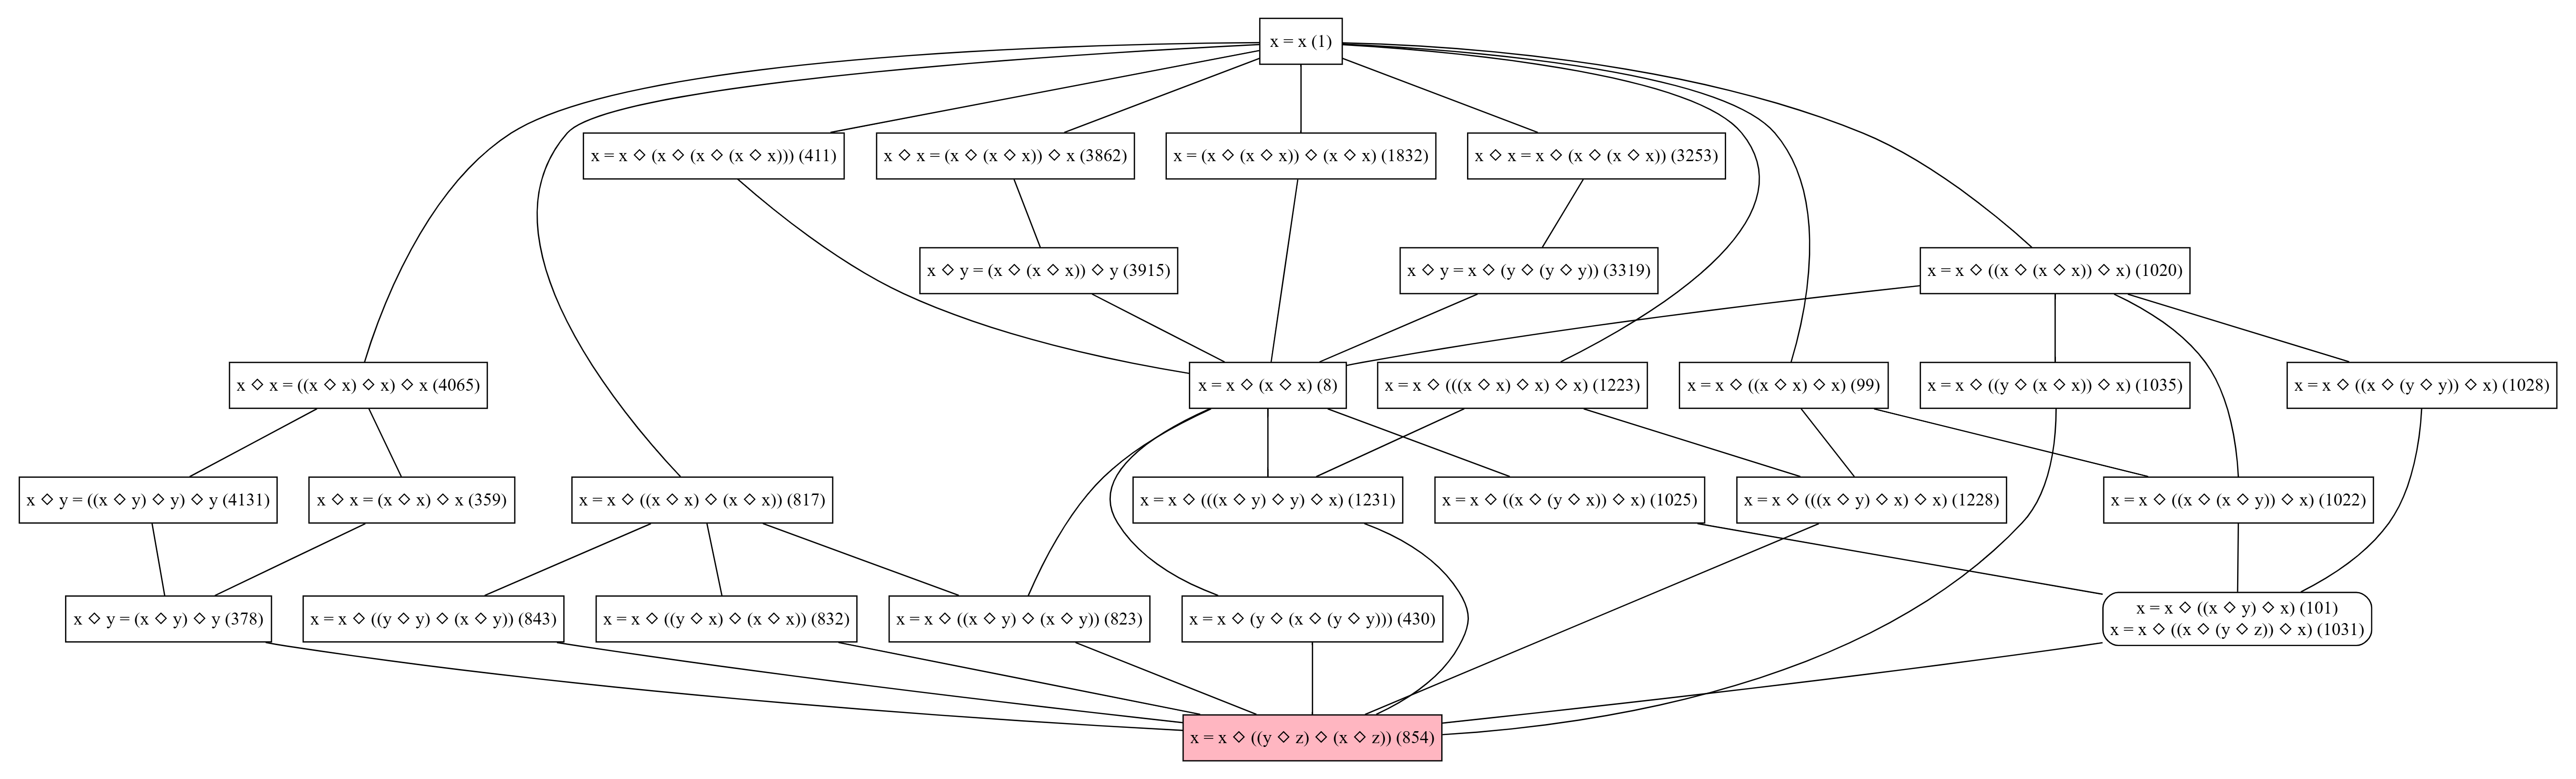
\includegraphics[width=0.85\textwidth]{854.png}
\caption{A Hasse diagram of all the equational laws implied by \eqref{eq854} (for unrestricted magmas).  An edge in this diagram indicates that the lower equation implies the higher one. Rounded rectangles indicate groups of equivalent laws.  This graph was produced by the visualization tool \emph{Graphiti}, which was developed for this project.}
\label{fig:854}
\end{figure}

\begin{figure}
    \centering
    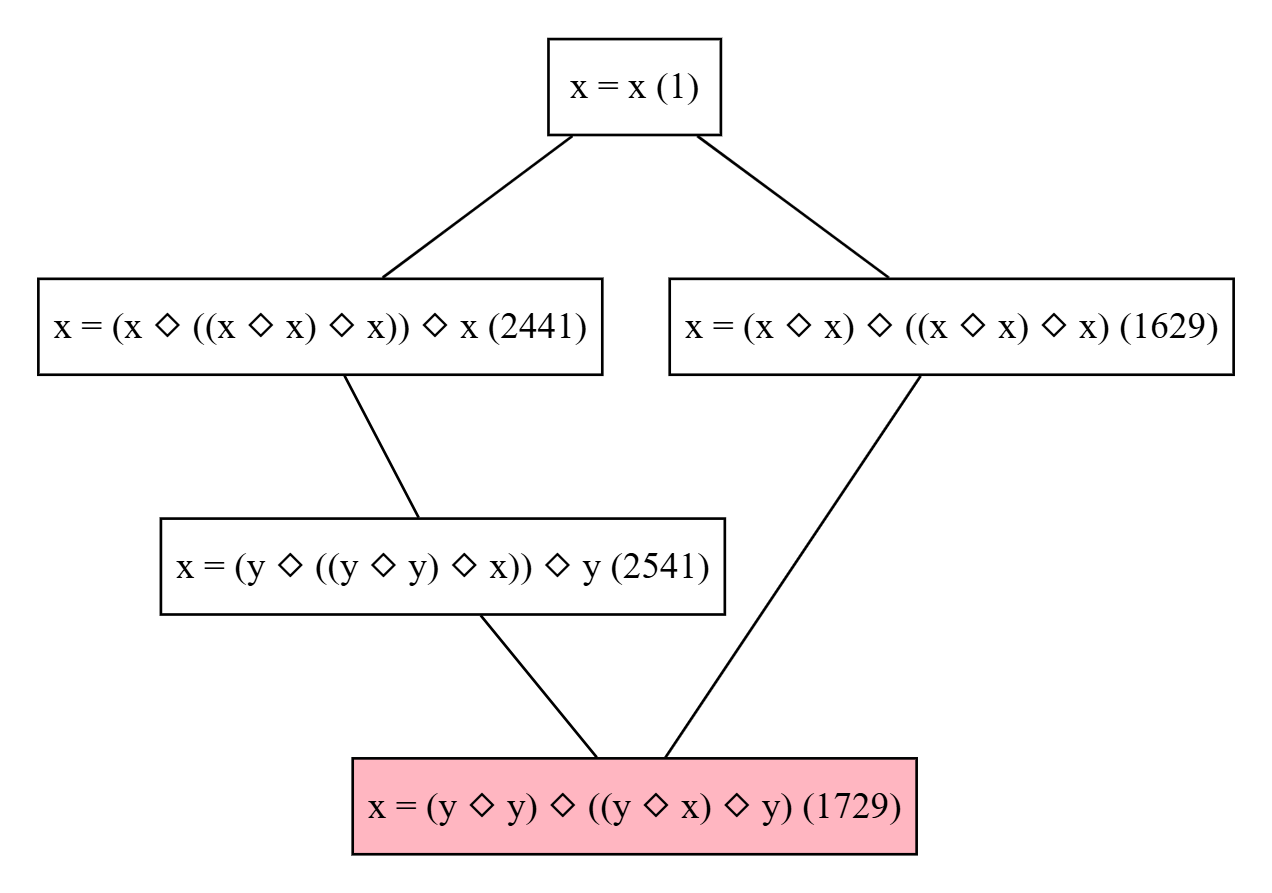
\includegraphics[width=0.4\textwidth]{ramanujan-infinite.png}
    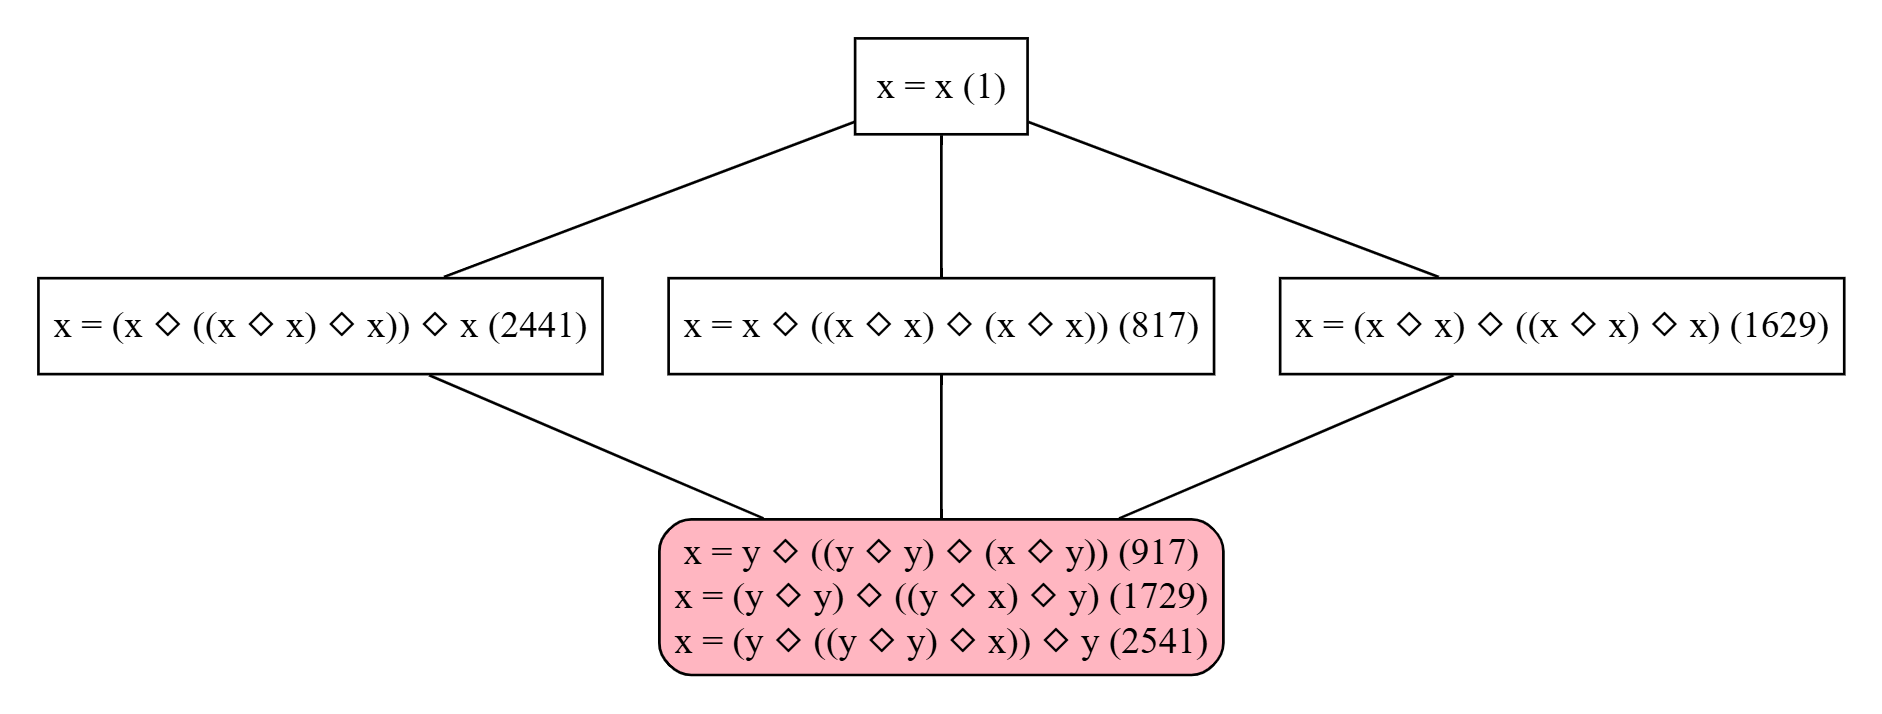
\includegraphics[width=0.4\textwidth]{ramanujan-finite.png}
    \caption{A Hasse diagram of all the equational laws implied by \eqref{eq1729}, both for unrestricted magmas (left) and finite magmas (right). Note the slightly larger number of implications in the latter.}
    \label{fig:1729}
\end{figure}

\begin{figure}
    \centering
    \resizebox{\textwidth}{!}{%
      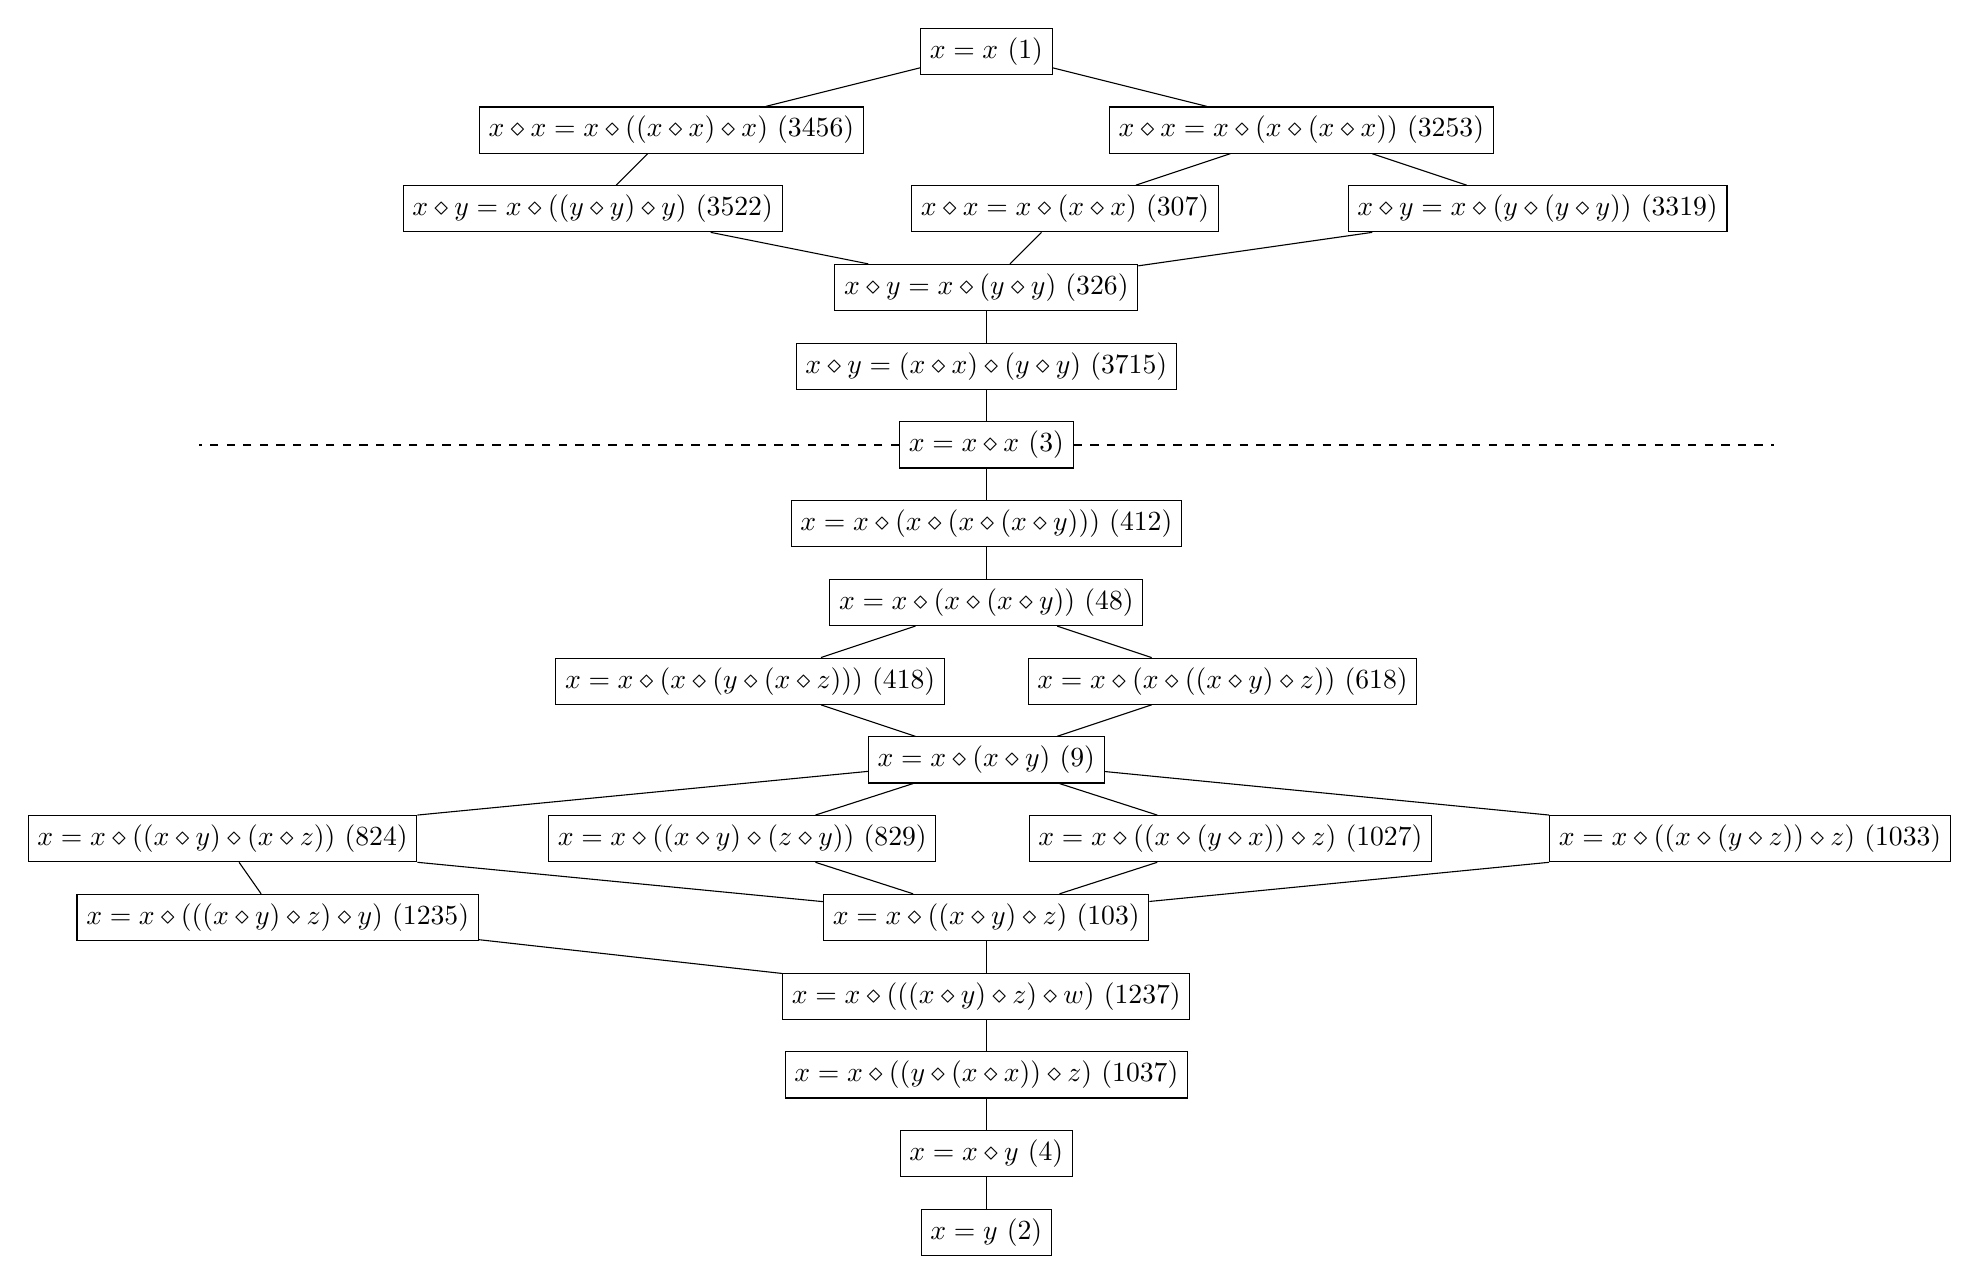
\begin{tikzpicture}
        \node(1)[draw] at (0,15) {$x = x$ (1)};
        \node(3253)[draw] at (4,14) {$x \op x = x \op (x \op (x \op x))$ (3253)};
        \node(3456)[draw] at (-4,14) {$x \op x = x \op ((x \op x) \op x)$ (3456)};
        \node(3319)[draw] at (7,13) {$x \op y = x \op (y \op (y \op y))$ (3319)};
        \node(307)[draw] at (1,13) {$x \op x = x \op (x \op x)$ (307)};
        \node(3522)[draw] at (-5,13) {$x \op y = x \op ((y \op y) \op y)$ (3522)};
        \node(326)[draw] at (0,12) {$x \op y = x \op (y \op y)$ (326)};
        \node(3715)[draw] at (0,11) {$x \op y = (x \op x) \op (y \op y)$ (3715)};
        \node(3)[draw] at (0,10) {$x = x \op x$ (3)};
        \draw[dashed](3)--(-10,10);
        \draw[dashed](3)--(10,10);
        \node(412)[draw] at (0,9) {$x = x \op (x \op (x \op (x \op y)))$ (412)};
        \node(48)[draw] at (0,8) {$x = x \op (x \op (x \op y))$ (48)};
        \node(618)[draw] at (3,7) {$x = x \op (x \op ((x \op y) \op z))$ (618)};
        \node(418)[draw] at (-3,7) {$x = x \op (x \op (y \op (x \op z)))$ (418)};
        \node(9)[draw] at (0,6) {$x = x \op (x \op y)$ (9)};
        \node(824)[draw] at (-9.7,5) {$x = x \op ((x \op y) \op (x \op z))$ (824)};
        \node(829)[draw] at (-3.1,5) {$x = x \op ((x \op y) \op (z \op y))$ (829)};
        \node(1027)[draw] at (3.1,5) {$x = x \op ((x \op (y \op x)) \op z)$ (1027)};
        \node(1033)[draw] at (9.7,5) {$x = x \op ((x \op (y \op z)) \op z)$ (1033)};
        \node(103)[draw] at (0,4) {$x = x \op ((x \op y) \op z)$ (103)};
        \node(1235)[draw] at (-9,4) {$x = x \op (((x \op y) \op z) \op y)$ (1235)};
        \node(1237)[draw] at (0,3) {$x = x \op (((x \op y) \op z) \op w)$ (1237)};
        \node(1037)[draw] at (0,2) {$x = x \op ((y \op (x \op x)) \op z)$ (1037)};
        \node(4)[draw] at (0,1) {$x = x \op y$ (4)};
        \node(2)[draw] at (0,0) {$x = y$ (2)};
        \draw(2)--(4);
        \draw(4)--(1037);
        \draw(1037)--(1237);
        \draw(1237)--(1235);
        \draw(1235)--(824);
        \draw(1237)--(103);
        \draw(103)--(1027);
        \draw(103)--(1033.south west);
        \draw(103)--(824.south east);
        \draw(103)--(829);
        \draw(1027)--(9);
        \draw(1033.north west)--(9);
        \draw(829)--(9);
        \draw(824.north east)--(9);
        \draw(9)--(418);
        \draw(9)--(618);
        \draw(418)--(48);
        \draw(618)--(48);
        \draw(48)--(412);
        \draw(412)--(3);
        \draw(3)--(3715);
        \draw(3715)--(326);
        \draw(326)--(3522);
        \draw(3522)--(3456);
        \draw(3456)--(1);
        \draw(326)--(307);
        \draw(307)--(3253);
        \draw(3253)--(1);
        \draw(326)--(3319);
        \draw(3319)--(3253);
      \end{tikzpicture}%
    }
    \caption{Longest chains of implications (length $15$) between inequivalent laws in the implication graph.  The parts above/below law 3 can be independently dualized. }
    \label{fig:longchain}
\end{figure}

Of the $\num{22033636}$ possible implications $E \vdash E'$, $8178279$ (or $37.12\%$) would end up being true; for an additional set of either $820$ or $822$ pairs $E,E'$, the weaker implication $E \vdashfin E'$ also held. To establish such positive implications $E \vdash E'$ or $E \vdashfin E'$, the main techniques used were as follows:

\begin{itemize}
    \item A very small number of positive implications were established and \textbf{formalized by hand}, mostly through direct rewriting of the laws; but this approach would not scale to the full project.
    \item \textbf{Simple rewriting rules}, for instance based on the observation that any law of the form $\x \formaleq f(\y,\z,\dots)$ was necessarily equivalent to the trivial law \eqref{eq2}, could already reduce the size of potential equivalence classes by a significant fraction. We discuss this method in \Cref{rewrite-sec}.
    \item The preorder axioms for $\vdash$, as well as the ``duality'' symmetry of the preorder with respect to replacing a magma operation $x \op y$ with its opposite $x \op^{\mathrm{op}} y \coloneqq y \op x$, can be used to significantly cut down on the number of implications that need to be proven explicitly; ultimately, only $10657$ ($0.13\%$) of the positive implications needed a direct proof.
    \item To obtain additional implications for finite magmas, heavy reliance was made on the fact that for functions $f \colon M \to M$ on a finite set $M$, surjectivity was equivalent to injectivity.  Some more sophisticated variants of this idea can lead to additional implications; see \Cref{finite-sec}.
    \item \textbf{Automated Theorem Provers} (ATP) could be deployed at extremely fast speeds to establish a complete generating set of positive implications; see \Cref{automated-sec}.
\end{itemize}

More challenging were the $\num{13855357}$ ($62.88\%$) implications that were false, $E \nvdash E'$, and particularly the slightly smaller set of $\num{13854535}$ or $\num{13854537}$ implications that were false even for finite magmas, $E \nvdashfin E'$. Here, the range of techniques needed to refute such implications were quite varied, and may be of independent interest:
\begin{itemize}
        \item \textbf{Syntactic methods}, such as observing a ``matching invariant'' of the law $E$ that was not shared by the law $E'$, could be used to obtain some refutations.  For instance, if both sides of $E$ had the same order, but both sides of $E'$ did not, this could be used to syntactically refute $E \vdash E'$.  Similarly, if the law $E$ was confluent, enjoyed a complete rewriting system, or otherwise permitted some understanding of the free magma associated to that law, one could decide the assertions $E \vdash E'$ for all possible laws $E'$, or at least a significant fraction of such laws.  We discuss these methods, and the extent to which they can be automated, in \Cref{syntactic-sec}.
        \item \textbf{Small finite magmas}, which can be described explicitly by multiplication tables, could be tested by brute force computations to provide a large number of finite counterexamples to implications, or by ATP-assisted methods. See \Cref{finite-sec}.
        \item \textbf{Linear models}, in which the magma operation took the form $x \op y = ax + by$ for some (commuting or noncommuting) coefficients $a,b$, allowed for another large class of counterexamples to implications, which could be automatically scanned for either by brute force or by Grobner basis type calculations; many of these examples could also be made finite. See \Cref{linear-sec}.
        \item \textbf{Translation invariant models}, in which the magma operation took the form $x \op y = x + f(y-x)$ on an additive group, or $x \op y = x f(x^{-1} y)$ on a noncommutative group, reduce matters to analyzing certain functional equations; see \Cref{translation-sec}.
        \item \textbf{Greedy methods}, in which either the multiplication table $(x,y) \mapsto x \op y$ or the function $f$ determining a translation-invariant model are iteratively constructed by a greedy algorithm subject to a well-chosen ruleset, were effective in resolving many implications not easily disposed of by preceding methods. See \Cref{greedy-sec}.
        \item Starting with a simple base magma $\Magma$ obeying both $E$ and $E'$, and either \textbf{enlarging} it to a larger magma $\Magma'$ containing $\Magma$ as a submagma, \textbf{extending} it to a magma $\MagmaN$ with a projection homomorphism $\pi: \MagmaN \to \Magma$, or \emph{modifying the multiplication table} on a small number of values, also proved effective when combined with greedy methods or with a ``\textbf{magma cohomology}'' construction. See \Cref{modify-base}.
        \item To each equation $E$ one can associate a ``\textbf{twisting semigroup}'' $S_E$.  If $S_E$ is larger than $S_{E'}$, then this can often be used to disprove the implication $E \vdash E'$; see \Cref{twisting-sec}.
        \item Some \textbf{ad hoc models} based on existing mathematical objects, such as infinite trees, rings of polynomials, or ``Kisielewicz models'' utilizing the prime factorization of the natural numbers, could also handle some otherwise difficult cases.  In some cases, the magma law induced some relevant and familiar structures, such as a directed graph or a partial order, which also helped guide counterexample constructions. We will not detail these diverse examples here, but refer the reader to the ETP blueprint for more discussion.
        \item \textbf{Automated theorem provers} were helpful in identifying which simplifying axioms could be added to the magma without jeopardizing the ability to refute the desired implication $E \vdash E'$ or $E \vdashfin E'$.
\end{itemize}

While the vast majority of negative implications could be quickly resolved by one of the above techniques, either with human input or in a completely automated fashion, there were perhaps two dozen such negative results that required quite delicate and \emph{sui generis} constructions.  The hardest such implication, $\Eq{1729} \nvdash \Eq{817}$, took several months to establish and then formalize (using a combination of many of the above constructions), with the final proof in \emph{Lean} requiring just over $\num{4000}$ dedicated lines of code from multiple contributors.

In the course of completing the implication graph, some interesting new algebraic structures were discovered.  One such example concerns the magmas obeying \eqref{eq1485}, which we refer to as \emph{weak central groupoids} as they contain the central groupoids (obeying \eqref{eq168}) as a subclass.  In \cite{knuth} it was observed that all finite central groupoids have order equal to a perfect square $n^2$; empirically, we have found that finite weak central groupoids always have order $n^2$ or $2n^2$, although we have no rigorous proof of this claim; they also have a graph-theoretic interpretation analogous to the interpretation of central groupoids as digraphs with the unique path property.  For these and other observations we refer the reader to \href{https://teorth.github.io/equational_theories/blueprint/weak-central-groupoids-chapter.html}{the blueprint of the ETP}.

The objective of using the data from the ETP to establish well-calibrated benchmarks to evaluate ATPs remains an interesting open problem; the participants of this project did not have the required expertise to develop and test such benchmarks to the standards expected in the area.  However, in \Cref{automated-sec} we present a more informal ``field report'' of our experiences using ATPs in the project, in the hope that this will provide some useful guidance to other researchers seeking to incorporate ATPs into their own research.

\begin{figure}
\centering
\begin{tikzpicture}[
    >=Latex,
    node distance=1.1cm,
    every node/.style={draw, rectangle, align=center},
    label/.style={font=\bfseries}
  ]

  %% Column labels
  \node[label] (ghlabel)   at (0,2) {GitHub};
  \node[label] (zuliplabel) at (7,2) {Lean Zulip};

  %% GitHub nodes
  \node (blueprint)   {Blueprint};
  \node (formal)     [below=of blueprint] {Lean formalization};
  \node (viz)        [below=of formal]    {Visualization tools};

  %% Lean Zulip nodes
  \node (hproofs)    [right=of blueprint]       {Human-gen. proofs};
  \node (cproofs)    [right=3cm of formal]         {Computer-gen. proofs};
  \node (hdisc)      [right=of viz]         {Human discussion};

  %% External ATP box
  \node (atp)        [right=of cproofs]         {ATPs, other\\external tools};

  %% Grouping boxes
  % GitHub container
  \node[draw,dotted,inner sep=8pt,fit=(blueprint)(formal)(viz), label=above:GitHub]
    (ghbox) {};
  % Lean Zulip container
  \node[draw,dotted,inner sep=8pt,fit=(hproofs)(cproofs)(hdisc), label=above:Lean Zulip]
    (zulipbox) {};

  %% Arrows
  \draw[human,->] (blueprint)  -- (formal);
  \draw[auto,->] (formal)     -- (viz);
  \draw[human,->] (viz)        -- (hdisc);
  \draw[human,->] (hdisc)      -- (atp);
  \draw[auto,->] (atp)        -- (cproofs);
  \draw[human,->] (cproofs)    -- (hproofs);
  \draw[semi,->] (cproofs)    -- (formal);
  \draw[human,<->] (hproofs)   -- (hdisc);
  \draw[human,->] (hproofs)  -- (blueprint);
  \draw[human,->] (hproofs)  -- (formal);

\end{tikzpicture}
\caption{Some of the main dynamics in which proofs were generated, discussed within the Lean Zulip channel and then formalized in the Github repository.  Boldface arrows indicate human activities, such as proposing an automated attack on outstanding implications, converting a computer-generated proof into a human-readable format, formalizing a human readable proof directly, or first creating a more precise blueprint for other collaborators to work on.  Dashed arrows indicate fully automated processes, while the partly dashed line indicated a semi-automated process requiring human supervision. }
\label{fig:flow}
\end{figure}

\subsection{Further directions}

While the primary objective of the ETP was being completed, some additional related results were generated as spinoffs.  Specifically:
\begin{itemize}
\item In the blueprint on the ETP web site, we report some partial progress on classifying which of the $57882$ distinct laws of order $5$ are equivalent to the singleton law \eqref{eq2}, either with or without the requirement that the magma be finite.
\item In \Cref{higman-neumann} we report on classifying the laws of order $8$ that are equivalent to the Higman-Neumann law \eqref{eq42323216}.
\item In \Cref{ml-sec} we report on preliminary experiments on using machine learning to determine to what extent the implication graph can be predicted by a neural network.
\end{itemize}

\section{Notation and Mathematical Foundations}\label{notation-sec}

If $\Magma = (M,\op)$ is a magma, we define the left and right multiplication operators $L_a, R_a \colon M \to M$ for $a \in M$ by the formula
\begin{equation}\label{left-right}
    L_x y = R_y x \coloneqq x \op y.
\end{equation}
We also define the squaring operator $S \colon M \to M$ by
\begin{equation}\label{square-def}
    Sx \coloneqq x \op x = L_x x = R_x x.
\end{equation}
%and the (right) cubing operator $C \colon M \to M$ by
%\begin{equation}\label{cube-def}
%    Cx \coloneqq Sx \op x = R_x^2 x.
%\end{equation}

A \emph{homomorphism} $f \colon \Magma \to \Magma'$ between two magmas $\Magma = (M,\op)$, $\Magma' = (M',\op')$ is a function $f \colon M \to M'$ such that $f(x \op y) = f(x) \op' f(y)$ for all $x,y \in M$.  An \emph{isomorphism} is a homomorphism that is invertible (which implies that the inverse is also a homomorphism).  An \emph{endomorphism} is a homomorphism from a magma to itself.

If $X$ is an alphabet, we let $\Magma_X$ denote the free magma generated by $X$, thus an element of $\Magma_X$ is either a letter in $X$, or of the form $w_1 \op w_2$ with $w_1,w_2 \in \Magma_X$.  Every function $f \colon X \to M$ into a magma $\Magma = (M,\op)$ extends to a unique homomorphism $\varphi_f \colon \Magma_X \to \Magma$.  Formally, an equational law with some indeterminates in $X$ can be written as $w_1 \formaleq w_2$ for some $w_1, w_2 \in X$; a magma $\Magma = (M,\op)$ then obeys this law if and only if $\varphi_f(w_1) = \varphi_f(w_2)$ for all $f \colon X \to M$.  We also define the order of a word $w \in \Magma_X$ to be the number of occurrences of $\op$ in the word, thus letters in $X$ are of order $0$, and the order of $w_1 \op w_2$ is the sum of the orders of $w_1, w_2$.

A \emph{theory} is a collection $\Gamma$ of equational laws; we say that a magma $\Magma$ \emph{satisfies} a theory, and write $\Magma \models \Gamma$, if every law in $\Gamma$ is obeyed by $\Magma$.  If $E$ is an equational law, we write $\Gamma \vdash E$ if every magma that satisfies $\Gamma$ also satisfies $E$. A \emph{free magma} $\Magma_{X,\Gamma}$ for such a theory $\Gamma$ and an alphabet $X$ is a magma satisfying $\Gamma$ together with a map $\iota_{X,\Gamma} \colon X \to \Magma_{X,\Gamma}$ which is universal in the sense that every function $f \colon X \to \Magma$ to a magma $\Magma$ satisfying $\Gamma$ uniquely determines a homomorphism $\varphi_{f,\Gamma} \colon \Magma_{X,\Gamma} \to \Magma$ such that $\phi_{f,\Gamma} \circ \iota_{X,\Gamma} = f$.  This magma is unique up to isomorphism; a canonical way to construct it is as the quotient $\Magma_X/\sim_\Gamma$ of the free magma $\Magma_X$ by the equivalence relation $\sim_\Gamma$ given by declaring $w \sim_\Gamma w'$ if $\Gamma \vdash w \formaleq w'$.  If $\Gamma = \{E\}$ consists of a single law $E$, we write $\Magma_{X,E}$, $\sim_E$, $\varphi_{f,E}$ for $\Magma_{X,\{E\}}$, $\sim_{\{E\}}$, $\varphi_{f,\{E\}}$ respectively . \note{Give reference for free magmas relative to theories}

In general, the free magma $\Magma_{X,\Gamma}$ is difficult to describe in a tractable form, but for some theories, one has a simple description:

\begin{example}[Commutative and associative free magma]\label{semi-group} The free magma $\Magma_{X,\{E43, E4512\}}$ for the commutative law \eqref{eq43} and the associative law \eqref{eq4512} is the free abelian semigroup generated by $X$ (with $\iota_{X,\{E43,E4512\}}$ the obvious embedding map).
\end{example}

\begin{example}[Left-absorptive free magma]\label{left-absorb}
The free magma $\Magma_{X,\{E4\}}$ for the left-absorptive law \eqref{eq4} is the magma with carrier $X$ and operation $x \op y = x$ (with $\iota_{X,E_4}$ the identity).
\end{example}


Every magma $\Magma$ has an opposite $\Magma^{\mathrm{op}}$, which has the same carrier but the opposite operation $x \op^{\mathrm{op}} y \coloneqq y \op x$.  A magma $\Magma$ obeys an equational law $E$ if and only if its opposite $\Magma^{\mathrm{op}}$ obeys the dual law $E^*$, defined by reversing the all operations.  For instance, the dual of
$\x \op \y \formaleq \x \op (\y \op \z)$ \eqref{eq327} is $\y \op \x \formaleq (\z \op \y) \op \x$, which in our numbering system we rewrite in normal form as $\x \op \y \formaleq (\z \op \x) \op \y$ \eqref{eq395}.

We then see that the implication graph has a duality symmetry: given two equational laws $E_1,E_2$, we have $E_1 \vdash E_2$ if and only if $E_1^* \vdash E_2^*$.

\section{Formal Foundations}

\note{TODO: expand this sketch.}

Here we describe the Lean framework used to formalize the project, covering technical issues such as:

\begin{itemize}
    \item Magma operation symbol issues
    \item Syntax (`LawX`) versus semantics (`EquationX`)
    \item "Universe hell" issues
    \item Additional verification (axiom checking, Leanchecker, etc.)
    \item Use of the `conjecture` keyword
    \item Use of namespaces to avoid collisions between contributions. (Note: we messed up with this with FreeMagma! Should have namespaced back end results as well as front end ones.)
    \item Use of Facts command to efficiently handle large numbers of anti-implications at once
\end{itemize}

Upstream contributions:

\begin{itemize}
    \item \href{https://github.com/leanprover-community/mathlib4/pulls?q=is%3Apr+is%3Abody+EquationalTheories+}{Mathlib contributions}
    \item \href{https://github.com/PatrickMassot/leanblueprint/pulls?q=is%3Apr+in%3Abody+EquationalTheories+}{LeanBlueprint contributions}
\end{itemize}

\section{Project Management}\label{project-sec}

\TODO{Shreyas Srinivas and Pietro Monticone have volunteered to take the lead on this section.}

This project is, among other things, an experiment on how to organise large scale collaborations for mathematical work. In this section, we describe several aspects of the mechanics of the collaborative effort.

\subsection{Problems of scale in mathematical collaboration}
In order to understand the difficulties of scaling that arise in large scale collaborations, it helps to revisit how traditional mathematical collaborations work and understand why they may not scale. Every collaboration is unique, and we cannot imagine that any universal template exists. However, some general patterns can be observed in any mathematical collaboration. Usually, a small number of contributors, usually under ten, who may know each other, join forces to tackle some class of problems. Typically the collaborators are academics who share substantial amounts of common knowledge. They discuss the problem at hand together, typically with some shared written medium such as a whiteboard. After several rounds of discussion and refinement, different members of the collaboration come up with different pieces of the solution and discuss how they fit together into a whole. Along the way, each collaborator writes out their specific contributions and reviews that of others. After several iterations of this process they synthesize the results into a single paper. At this point, the collaborators are reasonably confident about the correctness of their work, including theorem statements and proofs, and submit the paper for peer review. Of course, there are many variations to this general template, but the basic cycle of discuss, solve, write, cross-check, and revise process is always present in some form or another. Point 4 of the EMS code of practice for joint responsibility \cite{EMS_code_of_practice} explicitly specifies that the correctness of published work is the joint responsibility of all co authors.

However this project involved 50 contributors spread across the world, collaborating across several timezones and countries over the internet. The aforementioned process does not scale. Collaborators do not usually know each other nearly as well as they would in a traditional project. Further, as the number of contributors grows beyond the single digits, it becomes increasingly difficult to ensure that robustness of results. Joint responsibility implies that all authors ought to understand and check theorems and proofs written by everybody else. These issues are mitigated to a great extent by interactive theorem provers (hereon referred to as ITPs) can act as a common referee. ITPs of the LCF variety separate the proof generation and checking functionalities. Thus they allow a variety of methods of generating proofs, as long as those proofs are expressible in the samll langauge of the ITPs proof-checking kernel. However it is important to keep in mind that the subtleties implicit in the promise of ITPs:
\begin{itemize}
    \item However well checked and small, an ITPs proof-checking kernel could still contain fatal errors that falsely certifies incorrect proofs. These are rare, but not unheard of. ITPs are however carefully designed, implemented, and reviewed to mitigate this and the kernel is often kept small. For instance, the Lean ITP has a kernel implemented in under 10000 lines of code. \TODO{cite something here}
    \item An ITPs kernel checks whether a proof certificate constitutes a proof of a given theorem statement. It is important to remember that theorem statements are specified in a computer language which assigns a very specific meaning to eacb subexpression. They are in turn built on top of other definitions, that could could have unexpected meanings. A classic case is the definition of natural number subtraction in many type theoretic theorem provers, where a conscious design choice is made to assign the value 0 when the second argument is larger than the first.
\end{itemize}
\begin{itemize}
    \item Project generation from \href{https://github.com/pitmonticone/LeanProject}{template}
    \item GitHub issue management with \href{https://github.com/teorth/equational_theories/labels}{labels} and \href{https://github.com/users/teorth/projects/1}{task management dashboard}
    \item Continuous integration (builds, blueprint compilation, task status transition)
    \item Pre-push git hooks
    \item Use of blueprint (small note, see \#406: blueprint chapters should be given names for stable URLs)
    \item Use of Lean Zulip (e.g. use of polls)
\end{itemize}

Maybe give some usage statistics, e.g. drawing from \url{https://github.com/teorth/equational_theories/actions/metrics/usage}

Mention that FLT is also using a similar workflow.

\subsection{Handling Scaling Issues}

Also mention some early human-managed efforts ("outstanding tasks", manually generated Hasse diagram, etc.) which suffices for the first one or two days of the project but rapidly became unable to handle the scale of the project.

Mention that some forethought in setting up a GitHub organizational structure with explicit admin roles etc. may have had some advantages if we had done so in the planning stages of the project, but it was workable without this structure (the main issue is that a single person -- Terry -- had to be the one to perform various technical admin actions).

Use of transitive reduction etc.\ to keep the Lean codebase manageable. Note that the project is large enough that one cannot simply accept arbitrary amounts of Lean code into the codebase, as this could make compilation times explode. Also note somewhere that transitive completion can be viewed as directed graph completion on a doubled graph consisting of laws and their formal negations.

Technical debt issues, e.g., complications stemming from an early decision to make Equations.lean and AllEquations.lean the ground truth of equations for other analysis and visualization tools, leading to the need to refactor when AllEquations.lean had to be split up for performance reasons.

Note that the "blueprint" that is now standard for guiding proof formalization projects is a bit too slow to keep up with this sort of project that is oriented instead about proving new results. Often new results are stated and formalized without passing through the blueprint, which is then either updated after the fact, or not at all. So the blueprint is more of an optional auxiliary guiding tool than an essential component of the workflow.

\subsection{Other Design Considerations}

Explain what "trusting" Lean really means in a large project. Highlight the kind of human issues that can interfere with this and how use of tools like external checkers and PR reviews by people maintaining the projects still matters. Provide guidelines on good practices (such as branch protection or watching out for spurious modifications in PRs, for example to the CI). Highlight the importance of following a proper process for discussing and accepting new tasks, avoiding overlaps etc. These issues are less likely to arise in projects with one clearly defined decision maker as in this case, and more likely to arise when the decision making has to be delegated to many maintainers.

Note that despite the guarantees provided by Lean, non-Lean components still contained bugs. For instance, an off-by-one error in an ATP run created a large number of spurious conjectures, and some early implementations of duality reductions (external to Lean) were similarly buggy. "Unit tests", e.g., checking conjectured outputs against Lean-validated outputs, or by theoretical results such as duality symmetry, were helpful, and the Equation Explorer visualization tool also helped human collaborators detect bugs.

Meta: documenting thoughts for the future record is quite valuable. It would be extremely tedious to try to reconstruct real-time impressions long after the fact just from the GitHub commit history and Zulip chat archive.

\subsection{Maintenance}

Describe the role of maintainers and explain why they need to be conversant in the mathematics being formalised, as well as Lean. As such, the role of maintainers is often akin to postdocs or assistant profs in a research group who do some research of their own, but spend much of their time to guide others in performing their tasks, the key difference being that contributors are volunteers who choose their own tasks. Explain the tasks maintainers must perform. Examples:

\begin{itemize}
    \item Reviewing proofs,
    \item Helping with proofs and theorem statements when people get stuck,
    \item Offering suggestions and guidance on how to produce shorter or more elegant proofs,
    \item Ensuring some basic standards are met in proof blocks that make proofs robust to upstream changes,
    \item Creating and maintaining CI processes,
    \item Responding to task requests,
    \item Evaluating theorem and definition formulations (for example unifying many theorem statements into one using FactsSyntax),
    \item Suggesting better ones where possible,
    \item Ensuring that there is no excessive and pointless overlap of content in different contributions \TODO{elaborate on what level of overlap was permissible and what we consider excessive}.
\end{itemize}


\section{Counterexample constructions}

In this section we collect the various techniques developed in the ETP to construct counterexamples to various implications $E \vdash E'$.

\subsection{Finite magmas}\label{finite-sec}

A finite magma $\Magma$ of order $n$ can be labeled by the carrier $\{1,\dots,n\}$ and described by specifying the multiplication table $\op \colon \{1,\dots,n\} \times \{1,\dots,n\} \to \{1,\dots,n\}$.  By generating a list of all the equational laws $En$, $n=1,\dots,4694$ obeyed by this magma, one can create refutations: if $\Magma \models En$ and $\Magma \not \models Em$, then clearly $E_n \not \vdashfin E_m$ and hence also $E_n \not \vdash E_m$.  It is feasible to brute force over all $\sum_{n=2}^4 n^{n^2} \approx 4.3 \times 10^9$ non-trivial magmas of order at most $4$ to obtain many refutations of this type.
By performing brute force over all magmas up to order $4$, a total of $13,632,566$ implications ($61.9\%$ of all implications, and $96.3\%$ of the false ones) can be refuted with $524$ distinct magmas. Of these implications, $13,345,053$ were refuted with $3 \times 3$ magmas, with the remaining $415,293$ requiring $4 \times 4$ magmas. Performing this search took 165 CPU-hours.

However, it is not feasible to exhaustively search over the $5^{5^2} \approx 3 \times 10^{17}$ magmas of order $5$, even after quotienting out by isomorphism and symmetry (which roughly saves a factor of $5! \times 2 = 240$).  Randomly sampling such magmas did not produce significant refutations, as random magmas of order $5$ tended to obey few laws, and the set of laws covered were usually also exhibited by smaller magmas.  A more fruitful approach was to randomly sample from magmas with additional properties that encouraged satisfiability of a greater set of laws.  These included linear and quadratic magmas (discussed below), and cancellative magmas.  On the other hand, some classes of magmas, such as commutative magmas, ended up producing a disappointingly small number of additional refutations.

For specific refutations, it was sometimes possible to locate a finite example with an ATP, particularly if one also imposed additional axioms (e.g., an idempotence axiom $x = x \op x$) that one suspected would be useful.  For medium-sized magmas (of order $n=5,6,7,8$), this appeared to be a more efficient approach than brute force exhaustion of all such magmas.

\note{Discuss this further, perhaps give an example, or refer to the ATP section.  See also the discussion threads ``Counterexamples by enumerating words in quotient magmas'' and ``Using SAT solvers for model generation'' threads (sorry, LaTeX is choking on the URLs for some reason).}

It is a result of Kisielewicz \cite{Kisielewicz} that every law $En$ with $n \leq 4694$ is either equivalent to the singleton law $E2$, or else has a non-trivial finite model; in other words, the implications $En \vdash E2$ and $En \vdashfin E2$ are equivalent for $n \leq 4694$.  In fact our brute force search revealed that in the latter case there is always a model of order $2 \leq n \leq 5$, with the lone exception of \eqref{eq1286} (and its dual \eqref{eq2301}), for which the smallest non-trivial finite model was of order $7$, as presented in \Cref{1286-ex} below.  In fact, most of the 4694 laws either only had trivial models, or had an order 2 model, as shown in \Cref{size-table}.
\begin{table}
\centering
\begin{tabular}{ll}
  \hline
Order of smallest non-trivial model & Number of laws \\
\hline
Trivial only & $1496$ \\
$2$ & $3136$ \\
$3$ & $32$ \\
$4$ & $14$ \\
$5$ & $14$ \\
$7$ & $2$\\
\hline
\end{tabular}
\caption{Number of laws of order at most $4$ whose smallest non-trivial model is of a given size.}\label{size-table}
\end{table}
\subsection{Linear models}\label{linear-sec}

A fruitful source of counterexamples is the class of \emph{linear magmas}, where the carrier $M$ is a ring (which may be commutative or non-commutative, finite or infinite), and the operation $\op$ is given by $x \op y = ax + by$ for some coefficients $a,b \in M$; one can also generalize this slightly to \emph{affine magmas}, in which the operation is given by $x \op y = ax + by + c$, but for simplicity we shall focus on linear magmas here.  It is easy to see that in a linear magma, any word $w(x_1,\dots,x_n)$ of $n$ indeterminates also takes the linear form
$$ w(x_1,\dots,x_n) = \sum_{i=1}^n P_{w,i}(a,b) x_i$$
for some (possibly non-commutative) polynomial $P_{w,i}$ in $a,b$ with integer coefficients.  Thus, a linear magma will obey an equational law $w_1 \formaleq w_2$ if and only if the pair $(a,b)$ lies in the (possibly non-commutative) variety
\begin{equation}\label{variety}
  \{ (a,b) \in M \times M: P_{w_1,i}(a,b) = P_{w_2,i}(a,b) \hbox{ for all } i \}.
\end{equation}
As such, a necessary condition for such a law $w_1 \formaleq w_2$ to entail another law $w'_1 \formaleq w'_2$ is that one has the inclusion
$$ \{ (a,b) \in M \times M: P_{w_1,i}(a,b) = P_{w_2,i}(a,b) \hbox{ for all } i \} \subset
\{ (a,b) \in M \times M: P_{w'_1,i}(a,b) = P_{w'_2,i}(a,b) \hbox{ for all } i \} $$
for all rings $M$.  For commutative rings, this criterion can be checked by standard Grobner basis techniques; in the noncommutative case one can use methods such as the diamond lemma \cite{diamond-lemma}.

\begin{example}[Commutative counterexample]\label{1286-ex} For the law $x = y \op (((x \op y) \op x) \op y)$ \eqref{eq1286}, the variety \Cref{variety} can be computed to be
$$ \{ (a,b) \in M \times M: 1 = a+ba^3+bab, 0 = a + ba^2 b + b^2 \}$$
while the variety for the idempotent law \eqref{eq3} is
$$ \{ (a,b) \in M: a+b=1 \}.$$
Thus to show that \eqref{eq1286} does not entail \eqref{eq3}, it suffices to locate elements $a,b$ of a ring $M$ for one has $1 = a+ba^3+bab$, $0 = a + ba^2 b + b^2$, and $a+b \neq 1$.  Here one can take a commutative example, for instance when $M = \Z/p\Z$ and $(p,a,b) = (11,1,7)$ or $(p,a,b)=(7,6,2)$.
\end{example}

\begin{example}[Noncommutative counterexample]\label{1117-ex} For the law $x = y \op ((y \op (x \op z)) \op z)$ \eqref{eq1117}, the variety \Cref{variety} can be computed to be
$$ \{ (a,b) \in M \times M: 1 = baba, 0 = a+ba^2, 0 = bab^2 + b^2 \}$$
while the variety for $x = (x \op ((x \op x) \op x)) \op x$ \eqref{eq2441} is
$$ \{ (a,b) \in M \times M: a^2 + aba^2 + abab + ab^2 + b = 1 \}.$$
Observe that if $ba = -1$, then $(a,b)$ automatically lies in the first set, and lies in the second set if and only if $(ab+1)(b-1) = 0$.  One can then show that \eqref{eq1117} does not imply \eqref{eq2441} by setting $a = L$, $b = -R$ where $L, R$ are the left and right shift operators respectively on the ring of integer-valued sequences $\Z^\N$.  With some \emph{ad hoc} effort one can convert this example into a less linear, but simpler (and easier to formalize) example, namely the magma with carrier $\Z$ and operation $x \op y = 2x - \lfloor y/2 \rfloor$.
\end{example}

\begin{remark} As essentially observed in \cite{austin}, if there is a commutative linear counterexample to an implication $E \vdash E'$, then by the Lefschetz principle this counterexample can be realized in a finite field ${\mathbb F}_q$ for some prime power $q$ (and by the Chebotarev density theorem one can in fact take $q$ to be a prime, so that the carrier is of the form $\Z/p\Z$ for some prime $p$), so that one also has $E \vdashfin E'$.  As such, we have found that an effective way to refute implications by the commutative linear magma method is to simply perform a brute force search over linear magmas $x \op y = ax + by$ in $\Z/p\Z$ for various triples $(p,a,b)$. \note{Discuss performance of this method.}

On the other hand, the refutations obtained by non-commutative linear constructions need not have a finite model.  For instance, consider the refutation $E1117 \not \vdash E2441$ from \Cref{1117-ex}.  The law \eqref{eq1117} can be rewritten as $L_y R_z L_y R_z x = x$.  This implies that $R_z$ is injective and $L_y$ is surjective for all $y,z$.  For finite magmas $\Magma$, this then implies that the $L_y, R_z$ are in fact invertible, and hence we have also $R_z L_y R_z L_y x = x$, which implies \eqref{eq2441} by setting $x=y=z$.  Thus the refutation $E1117 \not \vdash E2441$ is ``immune'' to finite counterexamples.
\end{remark}

\begin{remark}  One can also consider nonlinear magma models, such as quadratic models $x \op y = ax^2 + bxy + cy^2 + dx + ey + f$ in a cyclic group $\Z/N\Z$.  For small values of $N$, we have found such models somewhat useful in providing additional refutations of implications $E \vdashfin E'$ beyond what can be achieved by the linear or affine models.  However, as the polynomials associated to a word $w(x_1,\dots,x_n)$ tend to be of high degree (exponential in the order of the word), it becomes quite rare for such models to obey a given equation $E$ when $N$ is large.
\end{remark}

\begin{remark} One can also consider the seemingly more general linear model $x \op y = ax + by$, where the carrier $M$ is now an abelian group, and $a,b$ act on $M$ by homomorphisms, that is to say that they are elements of the endomorphism ring $\mathrm{End}(M)$.  However, this leads to exactly the same varieties \Cref{variety} (where $M$ is now replaced by the endomorphism ring $\mathrm{End}(M)$) and so does not increase the power of the linear model for the purposes of refuting implications.
\end{remark}

\note{Give some statistics of what proportion of refutations can be resolved by linear models.}

On the other hand, there are certainly some refutations $E \not \vdash E'$ of implications that are ``immune'' to both commutative and non-commutative models, in the sense that all such models that obey $E$, also obey $E'$.  One such example is the refutation $E1485 \vdash E151$, which we discuss further in \Cref{twisting-sec} below.

\subsection{Translation-invariant models}\label{translation-sec}

It is natural to look for counterexamples amongst magmas that obey a large number of symmetries.  One such class of counterexamples are \emph{translation-invariant models}, in which the carrier $M$ is a group, and the left translations of this group form isomorphisms of the magma $M$.  In the case of an abelian group $M = (M,+)$, such models take the form
\begin{equation}\label{xop-add}
  x \op y = x + f(y-x)
\end{equation}
for some function $f \colon M \to M$; in the case of a non-abelian group $M = (M,\cdot)$, such models instead take the form
\begin{equation}\label{xop-mul}
x \op y = x f(x^{-1} y).
\end{equation}
For such models, the verification of an equational law in $n$ variables corresponds to a functional equation for $f$ in $n-1$ variables, as the translation symmetry allows one to normalize one variable to be the identity (say). This can simplify an implication to the point where an explicit counterexample can be found.  These functional equations are trivial to analyze when $n=1$.  For $n=2$, they are not as trivial, but still quite tractable, and has led to several refutations in practice.  The method does not appear to be particularly effective for $n>2$ due to the complexity of the functional equations.

\begin{example}[Abelian example]\label{abex}  For the law $\x \formaleq (\x \op \y) \op ((\x \op \y) \op \y)$ \eqref{eq1648}, we apply the abelian translation-invariant model \Cref{xop-add} with $y=x+h$ to obtain
\begin{align*}
  x \op y &= x + f(h) \\
  (x \op y) \op y &= x + f(h) + f(h-f(h)) \\
  (x \op y) \op ((x \op y) \op y) &= x + f(h) + f(f(h-f(h)))
\end{align*}
so that this law obeys \eqref{eq1648} if and only if the functional equation
$$f(h) + f(f(h-f(h))) = 0$$
holds for all $h \in M$.  Similarly, the law $\x \formaleq (\x \op (\x \op \y)) \op \y$ \eqref{eq206} is obeyed if and only if
$$ f(f(h)) + f(h - f(f(h))) = 0$$
for all $h \in M$.  One can now check that the function $f \colon \Z \to \Z$ defined by $f(h) \coloneqq - \mathrm{sgn}(h)$ (thus $f(h)$ equals $-1$ when $h$ is positive, $+1$ when $h$ is negative, and $0$ when $h$ is zero) obeys the first functional equation but not the second, thus establishing that $E1648 \not \vdash E206$.
\end{example}

\begin{example}[Non-abelian example]\label{trans-nonab}  We now obtain the opposite refutation $E206 \not \vdash E1648$ to \Cref{abex} using the non-abelian translation-invariant model.  By similar calculations to before, we now seek to find a function $f \colon M \to M$ on a non-abelian group $(M,\cdot)$ that obeys the functional equation
\begin{equation}\label{206-eq}
 f(f(h)) f(f(f(h))^{-1} h) = 1
\end{equation}
for all $h \in M$, but fails to obey the functional equation
\begin{equation}\label{1648-eq}
   f(h) f(f(f(h)^{-1} h)) = 1
\end{equation}
for at least one $h \in M$.  Now take $M$ to be the group generated by three generators $a,b,c$ subject to the relations $a^2=b^2=c^2=1$, or equivalently the group of reduced words in $a,b,c$ with no adjacent letters in the word equal.  We define
$$ f(1) = 1, f(a)=b, f(b) = c, f(c) = a$$
and then $f(aw)=a$ for any non-empty reduced word $w$ not starting with $a$, and similarly for $b$ and $c$.  The equation \eqref{206-eq} can be checked directly for $h=1,a,b,c$.  If $h=aw$ with $w$ non-empty, reduced, and not starting with $a$, then $f(f(h))^{-1} = f(f(h)) = b$ and $f(f(f(h))^{-1} h) = f(baw) = b$, giving \eqref{206-eq} in this case, and similarly for cyclic permutations. Meanwhile, \eqref{1648-eq} can be checked to fail for $h=a$.
\end{example}

\begin{remark}  The construction in \Cref{trans-nonab} also has the following more ``geometric'' interpretation.  The carrier $M$ can be viewed as the infinite $3$-regular tree, in which every vertex imposes a cyclic ordering on its $3$ neighbors (for instance, if we embed $M$ as a planar graph, we can use the clockwise ordering).  For $x,y \in M$, we then define $x \op y$ to equal $x$ if $x=y$.  If $y$ is instead a neighbor of $x$, we define $x \op y$ to be the next neighbor of $x$ in the cyclic ordering.  Finally, if $y$ is distance two or more from $x$, we define $x \op y$ to be the neighbor of $x$ that is closest to $y$.  One can then check that this model obeys \eqref{206-eq} but not \eqref{1648-eq}.
\end{remark}

\begin{remark} These constructions are necessarily infinitary in nature, because \eqref{eq206} and \eqref{eq1648} can be shown to be equivalent for finite magmas. Indeed, \eqref{eq206} can be written as $x = R_y L_x L_x y$, which implies that $R_y$ is surjective, hence injective, on a finite magma; writing $x = R_y z$ we conclude that $R_y z = R_y L_{z \op y} L_{z \op y} y$ and hence $z = L_{z \op y} L_{z \op y} y$, giving \eqref{eq1648}.  The opposite implication is similar (using \eqref{eq1648} to show that $R_y$ is injective, hence surjective), and is left to the reader.
\end{remark}

  Some refutations $E \not \vdash E'$ are ``immune'' by translation-invariant models, in that any translation-invariant model that obeys $E$, also obeys $E'$.  One obstruction is that for such models, the squaring map $S$ is necessarily an invertible map, since $Sx = x + f(0)$ in the abelian case and $Sx = xf(1)$ in the non-abelian case. On the other hand, adding the assumption of invertibility of squares can sometimes make the implication $E \vdash E'$.  For instance, the commutative law $\x \op (\y \op \y) \formaleq (\y \op \y) \op \x$ \eqref{eq4482} for a square and an arbitrary element will imply the full commutative law \eqref{eq43} for translation-invariant models due to the surjectivity of $S$, but does not imply it in general (as one can easily see by considering models where $S$ is constant).

\subsection{The twisting semigroup}\label{twisting-sec}

Suppose one has a magma $\Magma$ obeying a law $E$, that also enjoys some endomorphisms $T, U \colon \Magma \to \Magma$.  Then one can ``twist'' the operation $\op$ by $T,U$ to obtain a new magma operation
\begin{equation}\label{twist} x \op' y := Tx \op Uy.
\end{equation}
If one then tests whether this new operation $\op'$ obeys the same law $E$ as the original operation $\op$, one will find that this will be the case provided that $T,U$ obey a certain set of relations.  The semigroup generated by formal generators $\mathrm{T}, \mathrm{U}$ with these relations will be called the \emph{twisting semigroup} $\operatorname{Twist}_E$ of $E$.  This can be best illustrated with some examples.

\begin{example}  We compute the twisting semigroup of $\x \formaleq (\y \op \x) \op (\x \op (\z \op \y))$ \eqref{eq1485}.  We test this law on the operation \Cref{twist}, thus we consider whether
$$x = (y \op' x) \op' (x \op' (z \op' y))$$
holds for all $x,y,z \in M$.  Substituting in \Cref{twist} and using the homomorphism property repeatedly, this reduces to
$$x = (T^2y \op TUx) \op (UTx \op (U^2T z \op U^3y)).$$
If we impose the conditions $TU=UT$, $T^2 = U^3$, then this equation would follow from \eqref{eq1485} (with $x,y,z$ replaced with $TUx$, $T^2 y$, $U^2 Tz$ respectively).  Thus the twisting semigroup $\operatorname{Twist}_{E1485}$ of \eqref{eq1485} is generated by two generators $\mathrm{T}, \mathrm{U}$ subject to the relations $\mathrm{T} \mathrm{U}=\mathrm{U} \mathrm{T} = 1$, $\mathrm{T}^2 = \mathrm{U}^3$.  This is a cyclic group of order $5$, since the relations can be rewritten as $\mathrm{T}^5 = 1$, $\mathrm{U} = \mathrm{T}^{-1}$.

Now consider $\x \formaleq (\x \op \x) \op (\x \op \x)$ \eqref{eq151}.  Applying the same procedure, we arrive at
$$x = (T^2 x \op TUx) \op (UT x \op U^2 x)$$
so the twisting group $\operatorname{Twist}_{E151}$ is generated by two generators $\mathrm{T}, \mathrm{U}$ subject to the relations $\mathrm{T} \mathrm{U}=\mathrm{U} \mathrm{T} = \mathrm{T}^2 = \mathrm{U}^2 = 1$.  This is a cyclic group of order $2$, since the relations can be rewritten as $\mathrm{T}^2 = 1$, $\mathrm{U} = \mathrm{T}$.
\end{example}

Suppose the twisting semigroup $\operatorname{Twist}_E$ is not a quotient of $\operatorname{Twist}_{E'}$, in the sense that the relations that define $\operatorname{Twist}_{E'}$ are not obeyed by the generators of $\operatorname{Twist}_E$.  Then one can often disprove the implication $E \vdash E'$ by attempting the following procedure.
\begin{itemize}
\item First, locate a non-trivial magma $\Magma = (M,\op)$ obeying the law $E$.  Then the Cartesian power $M^{\operatorname{Twist}_E}$ of tuples $(x_W)_{W \in \operatorname{Twist}_E}$, with the pointwise magma operation, will also obey $E$.
\item Furthermore, this Cartesian power admits two endomorphisms $T, U$ defined by
$$ T (x_W)_{W \in \operatorname{Twist}_E} = (x_{W \mathrm{T}})_{W \in \operatorname{Twist}_E};
U (x_W)_{W \in \operatorname{Twist}_E} = (x_{W \mathrm{U}})_{W \in \operatorname{Twist}_E},$$
which obey the relations defining $\operatorname{Twist}_E$.
\item We now twist the magma operation $\op$ on $M^{\operatorname{Twist}_E}$ by $T,U$ to obtain a new magma operation $\op'$ defined by \Cref{twist}, that will still obey law $E$.
\item Because $T, U$ will not obey the relations defining $\operatorname{Twist}_{E'}$, it is highly likely that this twisted operation will not obey $E'$, thus refuting the implication $E \vdash E'$.  If $M$ and the twisting semigroup were finite, this approach should also refute $E \vdashfin E'$.
\end{itemize}

For instance, a non-trivial finite model for \eqref{eq1485} is given by the finite field $\mathbb{F}_2$ of two elements with the NAND operation $x \op y \coloneqq 1-xy$.  If we twist $\mathbb{F}_2^5$ by the left shift $T(x_i)_{i=1}^5 = (x_{i+1})_{i=1}^5$ and right shift $U(x_i)_{i=1}^5 = (x_{i-1})_{i=1}^5$, where we extend the indices periodically modulo $5$, then the resulting operation
$$ (x_i)_{i=1}^5 \op' (y_i)_{i=1}^5 \coloneqq (1 - x_{i+1} y_{i-1})_{i=1}^5$$
on $\mathbb{F}_2^5$ will still obey \eqref{eq1485}, but will not obey \eqref{eq151}, thus showing that $E1485 \not \vdashfin E151$ and hence $E1485 \not \vdash E151$.  This particular implication does not seem to be easily establishable by any of the other methods discussed in this paper.

\note{Report on how large the twisting semigroups are in practice, and how many implications can be refuted by this method.}


\subsection{Greedy constructions}\label{greedy-sec}

We have found \emph{greedy extension methods}, or \emph{greedy methods} for short, are a powerful way to refute implications, especially when the carrier $M$ is allowed to be infinite.  A basic implementation of this method is as follows.  To build a magma operation $\op \colon M \times M \to M$ that obeys one law $E$ but not another $E'$, one can first consider \emph{partial magma operations} $\op \colon \Omega \to M$, defined on some subset $\Omega$ of $M \times M$. Thus $x \op y$ is defined if and only if $(x,y) \in \Omega$. A magma operation is then simply a partial operation which is \emph{total} in the sense that $\Omega = M \times M$.  We say that a partial magma operation is \emph{finitely supported} if $\Omega$ is finite.

In the language of first-order logic, a partial magma operation can also be viewed as a ternary relation $R(x,y,z)$ on $M$ with the axiom that $R(x,y,z) \wedge R(x,y,z') \implies z=z'$ for all $x,y,z \in M$.  The support $\Omega$ is then the set of $(x,y)$ for which $R(x,y,z)$ holds for some (necessarily unique) $z$, which one can then take to be the definition of $z = x \op y$.

We say that one partial operation $\op' \colon \Omega' \to M$ \emph{extends} another $\op \colon \Omega \to M$ if $\Omega'$ contains $\Omega$, and $x \op y = x \op' y$ whenever $x \op y$ (and hence $x \op' y$) are defined. Given a sequence $\op_n \colon \Omega_n \to M$ of partial operations, each of which is an extension of the previous, we can define the \emph{direct limit} $\op_\infty \colon \bigcup_n \Omega_n \to M$ to be the partial operation defined by $x \op_\infty y \coloneqq x \op_n y$ whenever $(x,y) \in \Omega_n$.

Abstractly, the greedy algorithm strategy can now be described as follows.

\begin{theorem}[Abstract greedy algorithm]\label{greedy-abstract} Let $E,E'$ be equational laws, and let $\Gamma$ be a theory of first-order sentences regarding a  partial magma operations $\op \colon \Omega \to M$ on a carrier $M$.  Assume the following axioms:
\begin{itemize}
  \item[(i)] (Seed) There exists a finitely supported partial magma operation $\op_0 \colon \Omega_0 \to M$ satisfying $\Gamma$ that contradicts $E'$, in the sense that there is some assignment of variables in $E'$ in $M$ such that both sides of $E'$ are defined using $\op_0$, but not equal to each other.
  \item[(ii)]  (Soundness)  If $\op_n \colon \Omega_n \to M$ is a sequence of partial magma operations obeying $\Gamma$ with each $\op_{n+1}$ an extension of $\op_n$, and the direct limit $\op_\infty$ is total, then this limit obeys $E$.
  \item[(iii)] (Greedy extension)  If $\op \colon \Omega \to M$ is a finitely supported partial magma operation obeying $\Gamma$, and $a,b \in M$, then there exists a finitely supported extension $\op' \colon \Omega' \to M'$ of $\op$ to a possibly larger carrier $M'$ such that $a \op' b$ is defined.
\end{itemize}
Then $E \not \vdash E'$.
\end{theorem}

We remark that this greedy method seems to be inherently infinitary in nature, and does not seem well adapted to refute finite magma implications $E \vdashfin E'$.

\begin{proof}  We work on the countably infinite carrier $\N$.  By embedding the finitely supported operation $\op_0$ from axiom (i) into $\N$, we can assume without loss of generality that $\op_0$ has carrier $\N$.  By similar relabeling, we can assume in (iii) that $M' = M$ when $M=\N$, since any elements of $M' \backslash \N$ that
appear in $\Omega'$ can simply be reassigned to natural numbers that did not previously appear in $\Omega$.  We well-order the pairs in $\N \times \N$ by $(a_n,b_n)$ for $n=1,2,\dots$.  Iterating (iii) starting from $\op_0$, we can thus create a sequence of finitely supported magma operations $\op_0, \op_1, \dots$ on $\N$ obeying $\Gamma$, with each $\op_{n+1}$ an extension of $\op_n$, and $a_n \op_n b_n$ defined for all $n \geq 1$.  Then the direct limit $\op_\infty$ of these operations is total, and does not obey $E'$ thanks to axiom (i).  On the other hand, by axiom (ii) it obeys $E$, and the claim follows.
\end{proof}

We refer to $\Gamma$ as the \emph{rule set} for the greedy extension method. To apply \Cref{greedy-abstract} to obtain a refutation $E \vdash E'$, we have found the following trial-and-error method to work well in practice:
\begin{itemize}
\item[1.] Start with a minimal rule set $\Gamma$ that has just enough axioms to imply the soundness property for the given hypothesis $E$.
\item[2.] Attempt to establish the greedy extension property for this rule set by setting $a \op' b$ equal to a new element $c \not \in M$, and then defining additional values of $\op'$ as necessary to recover the axioms of $\Gamma'$.
\item[3.]  If this can be done in all cases, then locate a seed $\op_0$ refuting the given target $E'$, and STOP.
\item[4.]  If there is an obstruction (often due to a ``collision'' in which a given operation $x \op' y$ is required to equal two different values), add one or more rules to $\Gamma$ to avoid this obstruction, and return to Step 2.
\end{itemize}

As an example, we present

\begin{proposition}[73 does not imply 4380]\label{73-4380} The law $\x \formaleq \y \op (\y \op (\x \op \y))$ \eqref{eq73} does not imply $\x \op (\x \op \x) \formaleq (\x \op \x) \op \x$ \eqref{eq4380}.
\end{proposition}

\begin{proof} To build a rule set $\Gamma$ that will imply \eqref{eq73} when total, a natural first choice would be the single rule
\begin{itemize}
\item[1.] If $y \op (x \op y)$ is defined, then $y \op (y \op (x \op y))$ is defined and equal to $x$.
\end{itemize}
However, the greedy algorithm will fail just with this rule: if the partial operation has $x \op y$ and $z \op y$ both equal to some $w$ for some $x \neq z$, then any attempt to assign a value to $y \op w$ will lead to a contradiction, as the above rule will force $y \op w$ to equal both $x$ and $z$.  Indeed, it is clear that \eqref{eq73} forces all the right translation operators $R_y$ to be injective.  We therefore add this as an additional rule:
\begin{itemize}
\item[2.] If $x \op y$ and $z \op y$ are defined and equal, then $x=z$.
\end{itemize}
To avoid some unwanted edge cases, it is also convenient to impose the additional rule
\begin{itemize}
  \item[3.] If $x \op y$ is defined, it is not equal to $y$.
\end{itemize}
Unlike Rule 2, this rule is not forced by \eqref{eq73}, but can be enforced as part of the greedy construction.

The ruleset clearly obeys the soundness axiom (ii) of \Cref{greedy-abstract}.  We now verify the greedy extension axiom (iii).  Let $\Omega,a,b$ be as in that axiom. We may assume that $a \op b$ is undefined, since we are done otherwise. We adjoin a new element $c$ to $M$ to create $M'$, and set $a \op' b = c$.  If we also have $b = d \op a$ for some $d$ (unique by Rule 2, and only possible for $a \neq b$ by Rule 3), set $a \op' c = d$ (this is necessary to retain Rule 1).  Of course, we also set $x \op' y = x \op y$ whenever $x \op y$ is already defined.

Since $c \not \in M$, it is clear that $\op'$ is a finitely supported partial magma operation on $M'$.  It is also clear that $\op'$ obeys Rule 2 and Rule 3.   Now we case check Rule 1:
\begin{itemize}
\item Case 1: $x=c$ or $y=c$.  Not possible since no left multiplication with $c$ is defined.
\item Case 2: $x \op' y = c$.  Only possible when $x = a$, $y = b$, but then $y \op' (x \op' y)$ is undefined since $y = b \neq a$ if $d$ is defined.
\item Case 3. $y \op' (x \op' y) = c$.  Only possible when $y=a$ and $x=d$, and holds in this case.
\item Case 4: $x, y, x \op' y, y \op' (x \op' y) \neq c$: this case is covered by Rule 3 for $\op$.
\end{itemize}
To conclude, we need to locate a seed $\op_0$ obeying Rules 1,2,3 but contains a counterexample to \eqref{eq4380}.  One simple example is the carrier $\{0,1,2,3\}$ with $0 \op_0 0 = 1$, $0 \op_0 1 = 2$, $0 \op_0 2 = 0$, $1 \op_0 0 = 3$.
\end{proof}

This method is not guaranteed to halt in finite time, as there may be increasingly lengthy sets of rules one has to add to $\Gamma$ to avoid collisions.  However, in practice we have found many of the refutations that could not be resolved by simpler techniques to be amenable to this method (or variants thereof, as discussed below).

One can automate the above procedure by using ATPs (or SAT solvers) to locate new rules that are necessary and sufficient resolve any potential collision (and which, \emph{a posteriori}, can be seen to be necessarily consequences of the law $E$).  The seed-finding step (Step 3) is particularly easy to automate, and can also often be done by hand.  \note{Describe performance of this automated method.  Discuss the issue that some implications required a large SAT solver calculation that was difficult to formalize efficiently in Lean, prompting human-generated simplified proofs using smaller rulesets.}

However, in some cases we have found it necessary to add ``inspired'' choices of rules that were not forced by the initial hypothesis $E$, but which simplified the analysis by removing problematic classes of collisions from consideration.  We were unable to fully automate the process of guessing such choices; however, we found ATPs very useful for testing any proposed such guess.  In particular, if an ATP was able to show that the existing ruleset, together with a proposed new rule $A$, implied $E'$, then this clearly indicated that one should not add $A$ to the rule set $\Gamma$.  Conversely, if an ATP failed to establish such an implication, this was evidence that this was a ``safe'' rule to impose.

We also found that human verification of the greedy extension property was a highly error-prone process, as the case analysis often included many delicate edge cases that were easy to overlook.  Both ATPs and the Lean formalization therefore played a crucial role in verifying the human-written greedy arguments, often revealing important gaps in those arguments that required either minor or major revisions to the rule set.

The greedy method can also combined with the translation-invariant method, both in abelian and non-abelian settings. For instance, we can modify the proof of \Cref{greedy-abstract} to obtain the following variant:

\begin{theorem}[Non-commutative translation-invariant greedy algorithm]\label{nc-greedy-abstract} Let $F,F'$ be functional equations on groups, and let $\Gamma$ be a theory of first-order sentences regarding a partial function $f \colon \Omega \to G$ on a group $G = (G,\cdot)$.  Assume the following axioms:
  \begin{itemize}
    \item[(i)] (Seed) There exists a finitely supported partial function $f_0 \colon \Omega_0 \to G$ satisfying $\Gamma$ that contradicts $F'$, in the sense that there is some assignment of variables in $F'$ in $G$ such that both sides of $F'$ are defined using $f_0$, but not equal to each other.
    \item[(ii)]  (Soundness)  If $f_n \colon \Omega_n \to G$ is a sequence of partial functions obeying $\Gamma$ with each $f_{n+1}$ an extension of $f_n$, and the direct limit $f_\infty$ is total, then this limit obeys $F$.
    \item[(iii)] (Greedy extension)  If $f \colon \Omega \to G$ is a finitely supported partial function obeying $\Gamma$, and $a,b \in G$, then there exists a finitely supported extension $f' \colon \Omega' \to G'$ of $f$ to a possibly larger group $G'$ such that $a \op' b$ is defined.
  \end{itemize}
  Then $F \not \vdash F'$.
\end{theorem}

One can of course also develop an abelian analogue of the above theorem, in which $G = (G,+)$ and $G' = (G',+)$ are now required to be abelian.  We can then give an alternate proof of \Cref{73-4380} as follows:

\begin{proof}[Second proof of \Cref{73-4380}] (Sketch)  The functional equations associated to \eqref{eq73} and \eqref{eq4380} are
$f^2(h^{-1} f(h)) =h^{-1}$ and $f^2(1) = f(1) f(f(1)^{-1})$ respectively.  We apply \Cref{nc-greedy-abstract} with the following ruleset:
\begin{itemize}
  \item[1.]  If $f(h^{-1} f(h))$ is defined, then $f^2(h^{-1} f(h))$ is defined and equal to $h^{-1}$.
  \item[2.]  If $h^{-1} f(h)$ and $k^{-1} f(k)$ are defined and equal, then $h=k$.
  \item[3.]  If $f(h)$ is defined, it is not equal to $h$.
\end{itemize}
Axiom (ii) is clear.  To verify axiom (iii), we can assume $f(h)$ is undefined, then adjoin an element $c$ freely to $G$ to create a larger group $G'$, and set $f'(h) = c$.  If $h = k^{-1} f(k)$ for some $k$ (which is unique by Rule 2, and only possible for $h \neq 1$ by Rule 3), then also set $f'(c) = k^{-1}$.  One can then check that axiom (iii) is obeyed.  For axiom (i), take $G$ to be a free cyclic group with one generator $a$, and set $f(1) = a$, $f(a) = a^3$, $f(a^3) = 1$, $f(a^{-1}) = a^3$ (say).
\end{proof}

More complex (and \emph{ad hoc}) variants of the greedy algorithm are possible.  In some cases, we were not able to preserve the finitely supported nature of the partial operation or partial function, and needed to extend that partial object at an infinite number of values at each step.  In other cases, one also had to add additional temporary data during the greedy process to record tasks that one wished to attend to at a later stage of the process, but could not handle immediately because it was awaiting some other operation to become well-defined.  We will not attempt to survey all possible variants of this method here, but refer the reader to the ETP blueprint for further examples.

\subsection{Modifying base models}\label{modify-base}

A general technique that we have found useful in obtaining a refutation such as $E \not \vdash E'$ is to start with a simple base model $\Magma = (M,\op)$ that obeys both $E$ and $E'$, and modify it in various ways to preserve $E$, but create a violation of $E'$.  There are many such possible modifications, but three general ways that have proven effective are as follows:

\begin{itemize}
  \item[(i)]  Modify the magma operation $\op \colon M \times M \to M$ on a small set in order to violate $E'$, and then make further modifications as needed to recover $E$.
  \item[(ii)]  Construct an \emph{extension} $\MagmaN$ of $\Magma$, equipped with a surjective magma homomorphism $\pi: \MagmaN \to \Magma$, and defined in terms of some additional data.  Then solve for that data in such a way that $N$ obeys $E$ but not $E'$.
  \item[(iii)]  Construct an \emph{enlargement} $\Magma' = (M',\op')$ of $\Magma = (M,\op)$, which is a magma that contains $\Magma$ as a submagma.  One needs to construct the multiplication table $\op$ on $(M' \times M') \backslash (M \times M)$ in order to retain $E$ but disprove $E'$.
\end{itemize}

One appealing case of (ii), involving a ``magma cohomology'' analogous to (abelian) group cohomology, is that of an \emph{affine} extension of a magma ${\mathcal G} = (G,\op_G)$ by another magma $(M,\op_M)$ which is an abelian group $M$ with a linear magma operation $s \op_M t \coloneqq as + bt$ for some endomorphisms $a,b \in \mathrm{End}(M)$.  One can then consider extensions with carrier $G \times M$ and magma operation
\begin{equation}\label{xsyt}
 (x, s) \op (y, t) \coloneqq (x \op_G y, s \op_M t + f(x,y))
\end{equation}
for some function $f \colon G \times G \to M$.  If $(M,\op_M)$ and $(G,\op_G)$ already obey a law $E$, then this extension will also obey $E$ if and only if $f$ obeys a certain ``cocycle equation'', which is a linear equation on $f$.  One can then sometimes use linear algebra to locate an $f$ that obeys the cocycle equation for one law $E$ but not another $E'$, thus refuting the implication $E \vdash E'$.  An example is as follows:

\begin{proposition}[1110 does not imply 1629]\label{1110-1629} The law $\x \formaleq \y \op ((\y \op (\x \op \x)) \op \y)$ \eqref{eq1110} does not imply $\x \formaleq (\x \op \x) \op ((\x \op \x) \op \x)$ \eqref{eq1629}, even for finite magmas.
\end{proposition}

\begin{proof}  (Sketch) Using the linear ansatz, we find that \eqref{eq1110} has a model $\Magma$ with carrier $\F_5$ (the finite field $\Z/5\Z$) with operation $x \op y = 3x-y$.  We then apply the ansatz \eqref{xsyt} with $G=M$.  One then finds that this operation obeys \eqref{eq1110} if $f \colon \F_5 \times \F_5 \to \F_5$ obeys the cocycle equation
  $$3f(x,x) - 3f(y,2x) - f(3y-2x,y) + f(y,3y-x) = 0$$
for all $x,y \in \F_5$, and obeys \eqref{eq1629} if $f$ obeys the cocycle equation
$$ f(2x,0) - f(2x,2x) = 0$$
for all $x \in \F_5$.  A routine symbolic algebra package computation reveals that the space of $f$ that obeys the former equation is a six-dimensional vector space over $\F_5$, which is not contained in the solution space of the latter equation, giving the claim.
In fact, since these equations preserve the space of homogeneous polynomials of a fixed degree, one can use linear algebra to locate an example that is a homogeneous polynomial; one explicit choice is $$f(x,y) = y^5 +xy^4 + x^2y^3 +3x^3 y^2 + 3x^4 y_1$$.
\end{proof}

It may be of interest to develop this theory of ``magma cohomology'' further, for instance by defining higher order magma cohomology groups.

Now we give an example of how method (ii) can be combined with method (i).

\begin{proposition}[1659 does not imply 4315]\label{1659-4315} $\x \formaleq (\x \op \y) \op ((\y \op \y) \op \z)$ \eqref{eq1659} does not imply $\x \op (\y \op \x) \formaleq \x \op (\y \op \z)$ \eqref{eq4315}.
\end{proposition}

\begin{proof}  There are two simple models for \eqref{eq1659}: the model $G$ with carrier $\Z/2\Z$ and operation $x \op y = x+1$, and the model $\Magma$ with carrier $\Z$ and operation $x \op y = x$.  Using the ansatz \eqref{xsyt}, one can soon discover that one obtains a magma operation $\op: (G \times M) \times (G \times M) \to G \times M$ with $f(0,0)=f(1,0)=0$, $f(0,1)=-1$, and $f(1,1)=1$.  This model still obeys \eqref{eq4315}. However we can create a modification $\op'$ of $\op$ as follows.  We will seek to violate \eqref{eq4315} at $x = (0,0)$, $y = (0,0)$, $z = (1,0)$, thus we want
$$ (0,0) \op' ((0,0) \op' (0,0)) \neq (0,0) \op' ((0,0) \op' (1,0)).$$
We have $(0,0) \op (0,0) = (1,0)$ and $(0,0) \op (1,0) = (1,-1)$.  One can try to force the counterexample by setting $(0,0) \op' (1,0)$ to equal $(0,0)$ instead of $(1,-1)$. However, if this is the only change we make, then we no longer obey \eqref{eq1659}, since
$$ (1,0) \neq ((0,0) \op' (1,0)) \op' (((1,0) \op' (1,0)) \op (1,t))$$
for any $t \in \Z \backslash \{0\}$. But these are the only counterexamples created; and if one then sets $(0,0) \op' (1,t) = (0,0)$ for \emph{all} $t \in \Z$, then one can check that the modified operation $\op'$ now obeys \eqref{eq1659} but not \eqref{eq4315} as required.
\end{proof}

Finite models for the law $\x \formaleq \x \op ((\y \op \z) \op (\x \op \z))$ \eqref{eq854} seems to be somewhat ``mutable'' in that one can often change a small number of entries in the multiplication table, and also add an additional row and column to the table, in ways that preserve the law \eqref{eq854}.  This renders this law suitable for using methods (i), (iii) to construct new models of this equation that refute various implications $E854 \vdashfin E$, for instance by starting with a model that already refuted some stronger law $E'$, and attempt to modify it (possibly with ATP assistance) by some combination of methods (i), (iii) to then violate $E$. \note{Explain this in more detail}

Another way to utilize (iii), which proved useful for laws that involved the squaring operator $S$, was to adopt a ``squares first'' approach in which one selected a base model $S\Magma = (SM,\op)$ to serve as the set of squares, then extend it to a larger model $\Magma$ with carrier $M = SM \uplus N$ by first determining what the multiplication map should be on the diagonal $\{ (x,x): x\in N\}$ (i.e., to determine the squaring map $S \colon N \to SM$), together with the values on the blocks $SM \times N$, $N \times SM$, and then finally resolve the remaining values on the $N \times N$ block.  Often, versions of the greedy algorithm are useful for each of these stages of the construction.  The precise details are quite technical, particularly for the law $\x \formaleq (\y \op \y) \op ((\y \op \x) \op \y)$ \eqref{eq1729}, which was the last of the equations whose implications were settled by the ETP.  We refer the reader to the ETP blueprint for further details.


\section{Syntactic arguments}\label{syntactic-sec}

Many proofs or refutations of implications (or equivalences) between two equational laws $E,E'$ can be obtained from the syntactic form of the equation.  We discuss some techniques here that were useful in the ETP.

\subsection{Simple rewrites}\label{rewrite-sec}

Many equational laws $E'$ can be formally deduced from a given law $E$ by applying the Lean `rw' tactic to rewrite $E'$ repeatedly by some forward or backward application of $E$ applied to arguments that match some portion of $E$.  For instance, the commutative law \eqref{eq43} clearly implies $\x \op (\y \op \z) \formaleq (\y \op \z) \op \x$ \eqref{eq4531}
by a single such rewrite.  A brute force application of such rewrite methods is already able to directly generate about $15,000$ such implications, including many equivalences to the singleton law \eqref{eq2} and the constant law \eqref{eq46}.  After applying transitive closure, this generates about four million further such implications.

A simple observation that already generates many equivalences is that any equation of the form $\x \formaleq f(\y,\z,\dots)$ necessarily is equivalent to the trivial law $\x \formaleq \y$; similarly, an equation of the form $f(\x,\y) \formaleq g(\z,\w,\dots)$ implies $f(\x,\y) \formaleq f(\x',\y')$; and so forth. \note{Give some stats on how effective this is.}

\subsection{Matching invariants}

Fix an alphabet $X$. A \emph{matching invariant} is an assignment $I \colon \Magma_X \to {\mathcal I}$ of an object $I(w) \in {\mathcal I}$ in some space ${\mathcal I}$ to each word $w \in \Magma_X$ with the property that if an equational law $w_1 \formaleq w_2$ has matching invariants $I(w_1)=I(w_2)$, then the same matching $I(w'_1) = I(w'_2)$ holds for any consequence $w'_1 \formaleq w'_2$.  In particular, if one law $I(w_1)=I(w_2)$ and $I(w'_1) \neq I(w'_2)$, then the law $w_1 \formaleq w_2$ does not imply the law $w'_1 \formaleq w'_2$.

A simple example of a matching invariant is the multiplicity $(n_x)_{x \in X}$ of variables of a word: if $w_1,w_2$ have all variables $x$ appear the same number of times $n_x$ in both words, then any rewriting of a word $w$ using the law $w_1 \formaleq w_2$ will preserve this property.  Hence, if $w'_1, w'_2$ do not have that each variable appear the same number of times in both words, then $w_1 \formaleq w_2$ cannot imply $w'_1 \formaleq w'_2$.  For instance, the commutative law \eqref{eq43} cannot imply the left-absorptive law \eqref{eq4}.

One source of matching invariants comes from the free magma $\Magma_{X,\Gamma}$ of a theory:

\begin{proposition}[Free magmas and matching invariants]\label{free-inv}  Let $\Gamma$ be a theory, and let $\iota_{X,\Gamma} \colon X \to \Magma_{X,\Gamma}$ be the map associated to the free magma $\Magma_{X,\Gamma}$ for that theory.  Then the map $I \colon \Magma_X \to \Magma_{X,\Gamma}$ defined by $I(w) \coloneqq \varphi_{\iota_{X,\Gamma}}(w)$ is an invariant.
\end{proposition}

\begin{proof}  Suppose that $w_1 \formaleq w_2$ entails $w'_1 \formaleq w'_2$, and that $I(w_1) = I(w_2)$.  For any $f \colon X \to \Magma_{X,\Gamma}$, the two maps $\varphi_f, \varphi_{f,\Gamma} \circ \varphi_{\iota_{X,\Gamma}} \colon \Magma_X \to \Magma_{X,\Gamma}$ are both homomorphisms that extend $f$, hence agree by the universal property of $\Magma_X$, as displayed by the following commutative diagram:
\[\begin{tikzcd}
	&& X \\
	\\
	{\Magma_X} && {\Magma_{X,\Gamma}} && {\Magma_{X,\Gamma}}
	\arrow[hook, from=1-3, to=3-1]
	\arrow["{\iota_{X,\Gamma}}"', from=1-3, to=3-3]
	\arrow["f", from=1-3, to=3-5]
	\arrow["{I = \varphi_{\iota_{X,\Gamma}}}", from=3-1, to=3-3]
	\arrow["{\varphi_f}"', curve={height=18pt}, from=3-1, to=3-5]
	\arrow["{\varphi_{f,\Gamma}}", from=3-3, to=3-5]
\end{tikzcd}\]
In particular, the hypothesis $I(w_1)=I(w_2)$ implies that $\varphi_f(w_1) = \varphi_f(w_2)$ for all $f \colon X \to \Magma_{X,\Gamma}$; that is to say, the magma $\Magma_{X,\Gamma}$ obeys the law $w_1 \formaleq w_2$, and hence also $w'_1 \formaleq w'_2$ by hypothesis.  In particular, $\varphi_{\iota_{X,\Gamma}}(w'_1) = \varphi_{\iota_{X,\Gamma}}(w'_2)$, which gives $I(w'_1) = I(w'_2)$ as required.
\end{proof}

\begin{example}  If we take $\Gamma = \{E4\}$ to be the theory of the left-absorptive law \eqref{eq4} as described in \Cref{left-absorb}, then the matching invariant $I(w)$ produced by \Cref{free-inv} is the left-most letter of the alphabet $X$ appearing in the word; for instance $I((\x \op \y) \op \z) = \x$.  Thus, for example, the left-absorptive law \eqref{eq4} cannot imply the right-absorptive law \eqref{eq5}.
\end{example}

\begin{example}  If we take $\Gamma = \{E43, E4512\}$ to be the theory of the commutative law \eqref{eq43} and the associative law \eqref{eq4512}, then by \Cref{semi-group}, the associated invariant $I(w) = \sum_{x \in X} n_x e_x$ is the formal sum of all the generators $e_x$ appearing in the word $w$, in the free abelian semigroup generated by those generators.  This recovers the preceding observation that the multiplicities $(n_x)_{x \in X}$ form a matching invariant.
\end{example}

\begin{example}  Let $n \geq 1$ be a positive integer, and consider the theory $\Gamma = \{E43, E4512, E_n\}$ consisting of the previous theory $\{E43, E4512\}$ together with the order-$n$ law $L_x^y x = y$.  One can check that the free magma $\Magma_{X,\Gamma}$ can be described as the free group of exponent $n$ with generators $e_x, x \in X$, with associated map $\iota_{X,\Gamma} \colon x \mapsto e_x$.  The associated matching invariant $I(w) = \sum_{x \in X} n_x e_x$ is essentially the multiplicities $(n_x \hbox{ mod } n)_{x \in X}$ modulo $n$, which gives a slightly stronger criterion than the preceding matching invariant for refuting implications.  For example, the cubic idempotent law $\x \formaleq (\x \op x) \op \x$ \eqref{eq23}
has matching invariants $e_x = 3e_x$ in the $n=2$ case, and hence does not imply the idempotent law $\x \formaleq \x \op \x$ \eqref{eq3} since $e_x \neq 2e_x$ in the $n=2$ case.
\end{example}

\note{Give some statistics on how many refutations can be established by these methods.}

\begin{remark}  One can also obtain matching invariants from the free objects associated to theories that involve additional operations beyond the magma operation $\op$, such as an identity element or an inverse operation.  We leave the precise generalization of \Cref{free-inv} to such theories to the interested reader.
\end{remark}

\subsection{Confluence}

We briefly recall the basics of rewrite theory necessary to our exposition, following mostly Baader and Nipkow \cite{traat}, and generally omitting proofs when they can be found there.

We first work in the abstract taking an arbitrary set $A$, with a given equivalence relation over it which we denote $\approx$. We consider a relation $R$ over $A$.

\begin{definition}
  We write $a \rightarrow b$ if $a\ R\ b$ holds in $A$, and say that $a$ \emph{rewrites to} (or \emph{reduces to}) $b$. We further define
  \begin{itemize}
    \item $\rightarrow^+$ as the transitive closure of $R$.
    \item $\rightarrow^*$ as the reflexive transitive closure of $R$.
    \item $\leftrightarrow^*$ as the reflexive transitive and symmetric closure of $R$.
  \end{itemize}
  We sometimes write $b\leftarrow a$, (resp. $b\ {}^*\leftarrow a$ etc) to mean $a\rightarrow b$ (resp. $a\rightarrow^*b$ etc), and chain notations, e.g. $b_1\leftarrow a\rightarrow b_2$.
\end{definition}

Note that $\leftrightarrow^*$ is an equivalence relation and the hope is for it to be equal to $\approx$, in order to deduce properties of the latter.

One should first note that if even $R$ is contained in $\approx$, then so are $\rightarrow^+, \rightarrow^*$ and $\leftrightarrow^*$ (as it is an equivalence relation), so we will focus on that case. Generally $a \rightarrow^* b$ can be seen as a way to \emph{compute} the $\approx$ relation, as it is directed, in a way to constrain our search space.

However, in general, we cannot deduce the converse, so it may be the case that $a\approx b$ but neither $a\rightarrow^*b$ nor $b\rightarrow^*a$ nor even is there a single $c$ such that $a\rightarrow^* c\ {}^*\leftarrow b$, as the number of ``left-right alternations'' may be arbitrarily large.

The following properties are going to be very useful to deduce exactly such a converse.

\begin{definition}
  We say that $R$ is \emph{Church-Rosser} if whenever $a\leftrightarrow^* b$, there exists some $c$ such that
  \[a\rightarrow^* c\ {}^*\leftarrow b\]
  We say that $R$ is \emph{confluent} if whenever $b_1\ {}^*\leftarrow a\rightarrow^* b_2$ there exists some $c$ such that $b_1\rightarrow^* c\ {}^*\leftarrow b_2$.

  We say that $R$ is \emph{locally confluent} if whenever $b_1\leftarrow a\rightarrow b_2$ there exists some $c$ such that $b_1\rightarrow^* c\ {}^*\leftarrow b_2$.

  We say that (an arbitrary) $a$ is in \emph{normal form} (or $a$ is a normal form) if there is no $a' \neq a$ such that $a \rightarrow a'$, and that $R$ is \emph{weakly normalizing} if for every $a$, there is some $a'$ such that $a\rightarrow^*a'$ and $a'$ is in normal form.

  We say that $R$ is \emph{strongly normalizing} if there are no infinite rewrite sequences $a_1\rightarrow a_2\rightarrow \ldots$. In particular, a strongly normalizing $R$ is also weakly normalizing.
\end{definition}

It turns out that if $R$ is strongly normalizing and Church-Rosser, and effective (we can ``compute'' with it) then the problem of equivalence is decidable! This is because of the following lemma.

\begin{lemma}
  If $R$ is Church-Rosser, then any normal form is \emph{unique}.
\end{lemma}

This means that, in this situation, $a$ and $b$ reduce to an identical normal form $c$ \emph{if and only if} $a\leftrightarrow^* b$! This means that we have the following algorithm to decide $a\leftrightarrow^* b$ (and therefore $a\approx b$ if these relations coincide):
\begin{enumerate}
  \item Repeatedly apply $R$ to $a$ and $b$ until normal forms $a'$ and $b'$ are found for them (this is possible because $R$ is strongly normalizing).
  \item Compare $a'$ and $b'$ for exact equality (sometimes called ``syntactic equality'').
  \item If $a' = b'$, we can conclude $a\leftrightarrow^* b$.
  \item If $a' \neq b'$ can can conclude that they are \emph{not} equivalent due to the lemma.
\end{enumerate}

Note that weak normalization does not change much here except at step 1, where we need to pick reductions which eventually bring the elements to normal forms.

The strategy is therefore, for a given $\approx$ to find an $R$ which is (strongly) normalizing and Church-Rosser, and such that $\leftrightarrow^*\ =\ \approx$. This is roughly the goal of the entire field of \emph{completion}. We call such an $R$ \emph{complete for} $\approx$.

The task is helped by the following facts, which we state here also without proof.

\begin{theorem}
  \begin{enumerate}
    \item $R$ is Church-Rosser iff it is confluent.
    \item (Newman's lemma) if $R$ is strongly normalizing, then $R$ is confluent iff it is locally confluent.
  \end{enumerate}
\end{theorem}

This strategy can be leveraged by looking at the particulars of the equivalence relation of interest, namely quantified equations over syntactic trees as in \Cref{abstract-nonsense-chapter}, and a theory $\Gamma$, which we will usually take to be finite (usually it will have a single equation!).

We will therefore consider relations over the set of elements of the free magma $M_{X}$, and the aim is to find a rewrite system $R$ is complete for $\formaleq$.

Certainly $\formaleq$ is closed over substitutions, and be a \emph{congruence}: if $a\formaleq a'$ and $b\formaleq b'$ under $\Gamma$, then $a\op b\formaleq a'\op b'$ under $\Gamma$ as well.

We therefore consider $R$ to be both closed under substitutions and a congruence. A convenient way to represent this is via a \emph{rewrite system}: simply a set of pairs of words $(l, r) \in M_{X}$ (we typically write $l\rightarrow r$) which represents the smallest congruence, closed by substitutions that contains those pairs.

Naturally, a set of laws $w \formaleq w'$ can be seen, given a choice of orientation (left-to-right or right-to-left) for each law as such a rewrite system. In this case, it is very clear that the reflexive transitive closure $\leftrightarrow^*$ recovers the original equational theory $\Gamma\models \cdot\formaleq\cdot$. However, it's clear that sometimes these systems will either be not strongly normalizing, or confluent, or both.

For example, it's clear that commutativity (the rule $x\cdot y\formaleq y\cdot x$) cannot possibly be oriented in such a way as to be terminating. Here is a non-confluent example:

\[ x \cdot (y \cdot z) \rightarrow y \]
We have $a\cdot (b \cdot (c \cdot d)) \rightarrow^* b$, but also $a\cdot (b\cdot (c\cdot d))\rightarrow^* a\cdot c$ for any $a, b, c, d$ (which are all in normal form).

Knuth and Bendix \cite{knuth-bendix} described a technique by which a theory or set of equations $\Gamma$ could be turned into a complete system. The crucial idea is the observation that the non-local-confluence of a rewrite system can be reduced to a finite (if the system is finite) set of ``worst offenders'' for confluence. If these pairs can be \emph{joined} (reduced to the same term) then the system is confluent. It is possible to compute such pairs.

The high-level idea is therefore to identify such pairs, and add them as an unoriented equation, to be oriented if possible, and repeating until no un-joinable pairs exist. If this procedure succeeds and terminates, the system is successfully completed, and as a result the theory $\Gamma$ is decidable, via the completed system as described above.

We use the intuitive notions of ``position in a word'' and ``word at a position $p$''. We denote by $w[w']_p$ the word $w$ with $w'$ inserted at position $p$.

\begin{definition}
  Given a rewrite system $R$ and two rules $\rho_1: l_1\rightarrow r_1$ and $\rho_2: l_2\rightarrow r_2$ in $R$, we say that $(t, u)$ is a \emph{critical pair} for $\rho_1$ and $\rho_2$ if there is some non-variable position $p$ in $l_1$ such that $l_2$ unifies with the term at that position. We denote by $\sigma$ the most general unifier thus obtained and have $t = r_1\sigma$ and $u = l_1\sigma[r_2\sigma]_p$
\end{definition}

Note that, in the above setting, $t\leftarrow l_1\sigma\rightarrow u$, giving us a candidate for non-local-confluence. The next lemma states that these candidates are the most general ones.

\begin{theorem}
  Given a rewrite system $R$, if for every critical pair $(t, u)$ of $R$, there is a term $v$ such that $t\rightarrow^* v\ {}^*\leftarrow u$, then $R$ is locally confluent.
\end{theorem}

Note that building critical pairs of a finite system is computable. Therefore the only step of the completion process which require genuine creativity is the choice of the orientation of the equations, along with the proof that that orientation is strongly normalizing.

We note that even in the event that such an orientation is not found, one can still partially apply the completion procedure, using any well-founded order on terms that is stable by substitution and congruence, to obtain a semi-decision procedure for equality. This process is sometimes called \emph{unfailing completion} and is at the core of the \emph{superposition calculus} used in Vampire.

The associative and commutative laws, $x \op (y \op z) \sim (x \op y) \op z$ and $x \op y \sim y \op x$ both have confluent rewrite systems associated to them (by orienting the equations left-to-right). But it is easy to se that only the former has a complete rewrite system associated to it.

In addition it is easy to show, e.g. that $x \op (x \op x) \sim x$ has a natural orientation that is normalizing and such that the critical pairs are joinable, and hence is complete. This approach works for many rules.

It is easy to define a matching invariant for a complete system $R$ associated to $\Gamma$, by simply taking as model the elements of $\Magma_{X}$, the free magma without any relations, restricted to the elements $t \in \Magma_{X}$ that are irreducible under $R$. The interpretation function $\phi$ simply takes a term to its normal form (under $R$). The lemma above ensures that this is preserved under $\Gamma$.

\subsection{Unique factorization}

In general, the free magma $\Magma_{X,E}$ for a given equational law $E$, which we can canonically define as $\Magma_X / \sim_E$, is hard to describe explicitly; indeed, from the undecidability of implications between equational laws, such a magma cannot be computably described for arbitrary $E$.  Nevertheless, for some laws it is possible to obtain some partial understanding of $\Magma_{X,E}$ from a syntactic perspective.  For instance, if we can refute the equivalence $w'_1 \sim_E w'_2$ by constructing a counterexample magma $M$ that obeys $E$ but not $w'_1 \formaleq w'_2$, then this implies that the representatives $\iota_{X,E}(w'_1), \iota_{X,E}(w'_2)$ of  $w'_1, w'_2$ in $\Magma_{X,E}$ are distinct.

We illustrate this approach with equations $E$ of a left-absorptive form
\begin{equation}\label{left-absorptive}
\x \formaleq \x \op f(\x,\y,\z)
\end{equation}
for some word $f(\x,\y,\z)$, which imply the right-idempotent law \eqref{eq378}.

An illustrative example is the law \eqref{eq854} depicted in Figure \ref{fig:854}. Other examples are listed in \Cref{fig:854-like}.

\begin{figure}
  \centering
  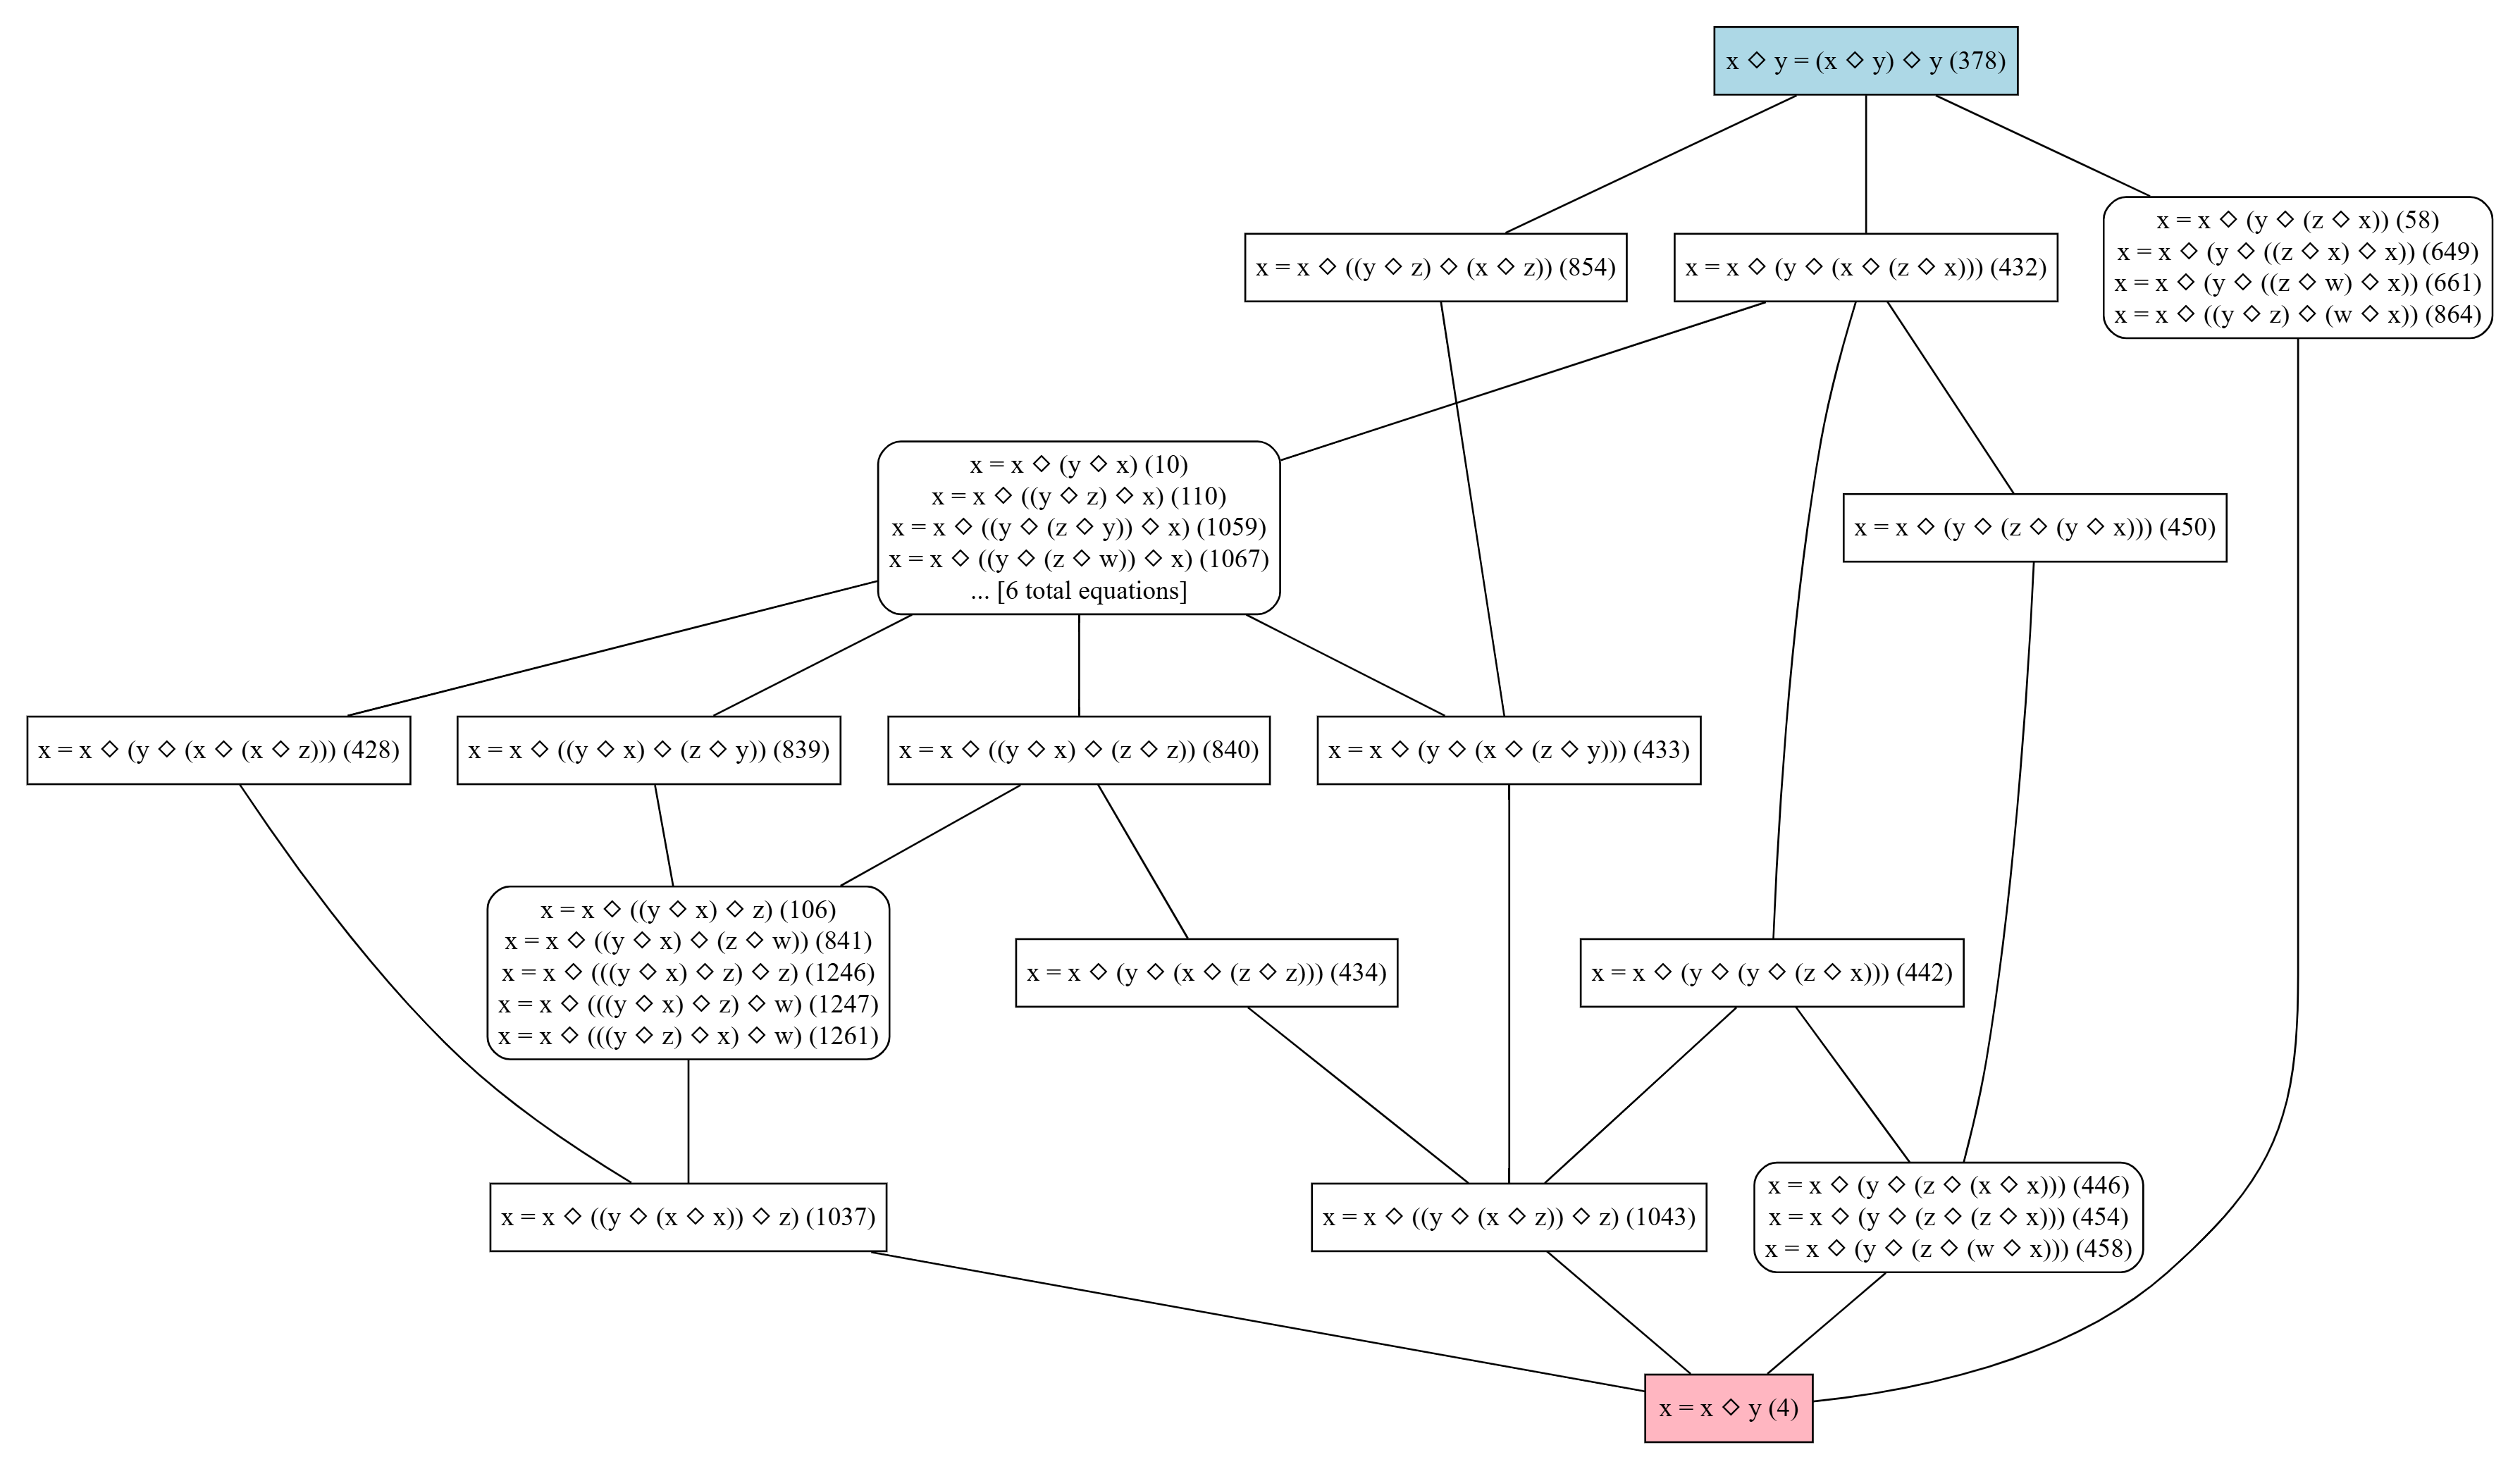
\includegraphics[width=0.85\textwidth]{854-like.png}
  \caption{Equations similar to \eqref{eq854} that are of the form \Cref{left-absorptive} (possibly involving a fourth indeterminate $\w$) and imply \eqref{eq378}.  For brevity, 70 equations equivalent to \eqref{eq4} have been omitted.}
  \label{fig:854-like}
  \end{figure}


\begin{lemma}\label{854} Equation \eqref{eq854} is of the form \Cref{left-absorptive} and implies \eqref{eq378}.
\end{lemma}

\begin{proof}  Clearly we have \Cref{left-absorptive} with $f(\x,\y,\z) \coloneqq (\y \op \z) \op (\x \op \z)$.  From \Cref{left-absorptive} we have in any magma obeying \eqref{eq854} that
$$x = x \op f(x,S^2 x,x) = x \op S(x \op S^2 x) = x \op S(x \op f(x,x,x)) = x \op Sx.$$
This implies from a further application of \Cref{left-absorptive} that
$$ y = y \op f(y,x,y) = (y \op Sy) \op ((x \op y) \op Sy) = f(x \op y, y, Sy)$$
and hence by \Cref{left-absorptive} again
$$ (x \op y) \op y = x \op y$$
giving \eqref{eq378}.
\end{proof}

Let $E$ be a law of the form \Cref{left-absorptive} that implies \eqref{eq378}. We define a directed graph $\to_E$ on words in $\Magma_X$ by declaring $w' \to_E w$ if $w \sim_E w'' \op w'$ for some $w' \in \Magma_X$.  By \eqref{eq378} (applied to the quotient magma $\Magma_{X,E} = \Magma_X/\sim_E$), this is equivalent to requiring that $w \sim_E w \op w'$. In particular, from \Cref{left-absorptive} we have $f(x,y,z) \to x$ for all $x,y,z$.  Furthermore, the relation $\to_E$ factors through $\sim_E$: if $w \sim_E \tilde w$ and $w' \sim_E \tilde w'$, then $w' \to_E w$ if and only if $\tilde w \to_E \tilde w$.

Call a word $w \in M_X$ \emph{irreducible} if it is not of the form $w = w_1 \op w_2$ with $w_2 \to_E w_1$.  We can partially understand the equivalence relation $\sim_E$ on irreducible words:

\begin{theorem}[Description of equivalence]\label{irred-desc}  Let $E$ be an equation of the form \Cref{left-absorptive}.  Let $w$ be an irreducible word, and let $w'$ be a word with $w \sim_E w'$.
  \begin{itemize}
    \item[(i)] If $w$ is a product $w = w_1 \op w_2$, then $w'$ takes the form
$$ w' = (((w'_1 \op w'_2) \op v_1) \op \dots \op v_n)$$
for some $w'_1 \sim_E w_1$, $w'_2 \sim_E w_2$, some $n \geq 0$, and some words $v_1, \dots, v_n$ such that for all $0 \leq i < n$, $v_{i+1}$ is of the form
$$ v_{i+1} \sim_E f(x_i,y_i,z_i)$$
for some $x_i, y_i, z_i$ with
$$ x_i \sim_E (((w'_1 \op w'_2) \op v_1) \op \dots \op v_i).$$
In particular, $v_{i+1} \to_E x_i$.
  \item[(ii)] Similarly, if $w \in X$ is a generator of $M_X$, then $w'$ takes the form
$$ w' = ((w \op v_1) \op \dots \op v_n)$$
for some $n \geq 0$, and some words $v_1, \dots, v_n$ such that for all $0 \leq i < n$, $v_{i+1}$ is of the form
$$ v_{i+1} \sim_E f(x_i,y_i,z_i)$$
for some $x_i, y_i, z_i$ with
$$ x_i \sim_E ((w \op v_1) \op \dots \op v_i).$$
In particular, $v_{i+1} \to_E x_i$.
\end{itemize}
Conversely, any word of the above forms is equivalent to $w$.
\end{theorem}

\begin{proof}  We just verify claim (i), as claim (ii) is similar.  The converse direction is clear from \Cref{left-absorptive} (after quotienting by $\sim_E$), so it suffices to prove the forward claim. By the Birkhoff completeness theorem, it suffices to prove that the class of words described by (i) is preserved by any term rewriting operation, in which a term in the word is replaced by an equivalent term using \Cref{left-absorptive}.  Clearly the term being rewritten is in $w'_1$ or $w'_2$ then the form of the word is preserved, and similarly if the term being rewritten is in one of the $v_i$.  The only remaining case is if we are rewriting a term of the form
$$ x_i = (((w'_1 \op w'_2) \op v_1) \op \dots \op v_i).$$
If $i>0$ we can rewrite this term down to $x_{i-1}$, and this still preserves the required form (decrementing $n$ by one).  If $i=0$ then we cannot perform such a rewriting because of the irreducibility of $w_1 \op w_2$ and hence $w'_1 \op w'_2$.  Finally, we can rewrite $x_i$ to $x_i \op v$ where $v$ is of the form
$$ v_i = f(x_i,y,z),$$
and after some relabeling we are again of the required form (now incrementing $n$ by one). This covers all possible term rewriting operations, giving the claim.
\end{proof}

Specializing to the case where $w,w'$ are both irreducible, we conclude

\begin{corollary}[Unique factorization]\label{unique factorization}  Two irreducible words $w, w'$ are equivalent if and only if they are either the same generator of $X$, or are of the form $w = w_1 \op w_2$, $w' = w'_1 \op w'_2$ with $w_1 \sim_E w'_1$ and $w_2 \sim_E w'_2$.
\end{corollary}

As an application of this corollary, we establish

\begin{proposition}[E854 does not imply E3316]\label{854-3316} Equation \eqref{eq854} does not imply \eqref{eq3316}.
\end{proposition}

\begin{proof}(Sketch)
  We work in the free group $\Magma_X$ on two generators $X = \{\x,\y\}$.  It suffices to show that
$$  \x \op \y \not \sim_{E854} \x \op (\y \op (\x \op \y)).$$
Suppose this were not the case, then by \Cref{unique factorization} one of the following statements must hold:
\begin{itemize}
\item[(i)] $y \to_{E854} x$.
\item[(ii)] $(y \op (x \op y)) \to_{E854} x$.
\item[(iii)] $y \op (x \op y) \sim_{E854} y$.
\end{itemize}
If (i) holds, then we have $x \op y = x$ must hold in $\Magma_X/\sim_E$, hence \eqref{eq854} would imply \eqref{eq4}.  However, it is possible to refute this implication by a finite counterexample.

Similarly, if (iii) held, then \eqref{eq854} would have to imply \eqref{eq10}, but this can also be refuted by a finite magma.

Finally, if (ii) held, then the claim
$$  x \op y \sim x \op (y \op (x \op y))$$
to refute simplifies to
$$  x \op y \sim x$$
and we are back to (i), which we already know not to be the case.
\end{proof}

\section{Proof Automation}\label{automated-sec}

In this project we used proof automation in two ways: automated theorem provers (ATPs) and Lean tactics.
ATPs are generally stand-alone tools that implement a (semi-) decision procedure for a given formal language or related set of languages.
For example, Vampire~\cite{DBLP:conf/cav/KovacsV13} is an ATP focused primarily on first-order logic using superposition, which we used extensively in this project.

ATPs are complex software that can contain bugs.
Instead of trusting ATP output, we used proof certificates, which many ATPs can produce, to reconstruct a proof in Lean.
This process depends on the proof certificate and the ATP, and we describe it for the main reconstruction we have done.

Tactics in Lean, on the other hand, are meta-programs~\cite{DBLP:journals/pacmpl/EbnerURAM17} that builds proofs.
In other words, tactics are programs that operate at the meta-level of Lean code: they essentially take in Lean code as input and produce Lean code as output.
In this manner, they look like another keyword in the language, and are tightly integrated by producing proofs directly.
Under the hood, they can implement essentially anything, from syntactic sugar to full decision procedures.
The \texttt{duper} tactic~\cite{DBLP:conf/itp/CluneQBA24}, for example, implements a superposition calculus, similar to Vampire's, but for dependent types --- Lean's underlying logical foundation.

In the rest of this section we describe the different proof automation techniques and ATPs/tactics we used.
We first discuss the different proof methods used: primarily superposition and equational reasoning, we then discuss the integration in Lean, and finally we report some basic empirical results from this project.

\subsection{Proof Techniques}

The main two families of ATPs and tactics we used here are superposition/saturation-based and equational reasoning ones.
In this context we also include SMT solvers, which combine specific decision procedures for theories, like congruence closure for equational reasoning, with satisfiability (SAT) solving~\cite{}.
Finally, we also used \texttt{aesop}~\cite{DBLP:conf/cpp/LimpergF23}, which implements a version of tableau search.
This was used mainly to help specific constructions in refutations, and is not specific to proving or disproving magma implications in this sense.
We will describe our use of \texttt{aesop} more in Section~\ref{sec:proof-reconstruction} below.

\paragraph{Saturation}
Most of the ATPs we used extensively in this project rely primarily on saturation procedures in the superposition calculus.
This is the case for Vampire~\cite{DBLP:conf/cav/KovacsV13}.
See also~\cite{DBLP:journals/cacm/BentkampBNTVW23} for a gentler exposition.
The core idea of these provers is that they take a set of assumptions and conjecture, expressed in --- say --- first-order logic.
They take the conjecture and negate it, adding this negation to the set of assumptions, which are all put in some normal form.
The ATP then tries to refute the negation by applying rules of the underlying calculus, until they find a proof of false (a contradiction).
In this case, the conjecture was (classically) true, and the ATP has found a proof by contradiction, often called a ``refutation'' or ``saturation'' proof.

The underlying calculus varies from system to system, but they often have a variant of a resolution clause, a clause of a form:
\[\infer{C \lor D}{C \lor L \quad D \lor \neg L} \]
This can also be read as $C \lor L \quad D \lor \neg L$ implies $C \lor D$, where $C, D, L$ are formulas in e.g. first-order logic.
Superposition calculi have a variant of this rule that deals with equality directly, and thus are more efficient at reasoning about equality.

In this project we used Vampire~\cite{DBLP:conf/cav/KovacsV13}, Duper~\cite{DBLP:conf/itp/CluneQBA24} and Prover9 and Mace4~\cite{prover9-mace4} which are all based on variants of saturation for proving.
TODO: here we could add a screenshot of using vampire or prover9.

\paragraph{Equational Reasoning}

Equational reasoning is a type of reasoning based on equational logic and rewriting with congruence~\cite{term-rewriting}, see Chapter~\ref{todo} for a discussion of its foundations in universal algebra.
In general, it takes a series of equations and determines wether another equation can be deduced from it.
A core tool in equational reasoning are e-graphs, a data structure used to represent equivalence classes of terms.
The procedure of congruence closure that can be used to decide ground equational problems (i.e. problems without variables) and as a semi-decision procedure in general.

SMT solvers like Z3~\cite{DBLP:conf/tacas/MouraB08} use equational reasoning for deciding the theory of equality with uninterpreted functions~\cite{DBLP:series/txtcs/KroeningS16,DBLP:conf/cade/MouraB07}.
On the other hand, equality saturation~\cite{DBLP:journals/pacmpl/WillseyNWFTP21} uses e-graphs by extending congruence closure to a more controlled search, enabling optimization and conditional rewriting.
One of the main advantages of using equational reasoning to reason about implications of magma laws is that we get very explicit proofs: a proof that $l \vdash l'$ is given by a sequence of rewrites that starts at the left-hand side of $l'$ and arrives at the right-hand side through applications of $l$.

In this project we used Z3~\cite{DBLP:conf/tacas/MouraB08}, Prover9 and Mace4~\cite{prover9-mace4}, a custom ATP for magmas based on egg~\cite{DBLP:journals/pacmpl/WillseyNWFTP21}, and the Lean egg tactic~\cite{DBLP:journals/pacmpl/KoehlerGBGTS24,rossel2024bridging}, which all work with equational logic. We have also reasoned with manual (custom written) heuristics about simple rewrites.

\subsection{Proof Reconstruction and Integration}
\label{sec:proof-reconstruction}

While ATPs are very useful to solve questions for this project, they generally don't integrate well with Lean .
A bug in an ATP could lead to an unsound proof, or worse, an incorrect result.
To avoid this, and having to trust large codebases from ATPs, we take results found by the different provers and (re-)construct proofs in Lean.

An exception for this are tactics like \texttt{duper}, \texttt{aesop} and \texttt{egg}). Figure~\ref{fig:screenshot-egg} shows an example of the \texttt{egg} tactic as used in this project. It integrates directly in Lean, generating a Lean proof directly. With the variant \texttt{egg?}, depicted in the screenshot, it uses an auxilariy tactic \texttt{calcify}\footnote{\url{https://github.com/nomeata/lean-calcify}} to generate a human-readable proof as a series of calculation steps, which can be incorporated into the file with a single click.

\begin{figure}
  \centering
  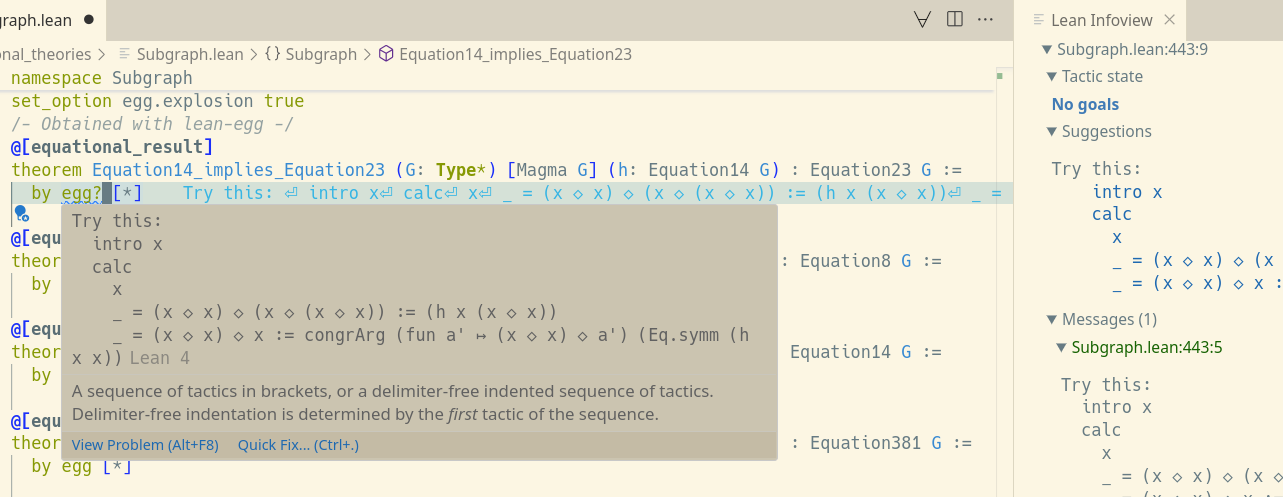
\includegraphics[width=0.85\textwidth]{screenshot-egg.png}
  \caption{An example of the use of proof automation with tactics. This shows the egg tactic as it was used to generate (human-readable) equational proofs of positive implications.}
  \label{fig:screenshot-egg}
\end{figure}

In general, integration implies two steps: invoking the decision procedures/ATPs (translating the problem from Lean into the languages and logics they use), and conversely, (re-)constructing the results from the decision procedure as a (persistent) Lean proof.
These two aspect present different challenges, and require different strategies, depending mostly on the kind of proof strategy the decision procedure uses.

For saturation proofs $\ldots$ (TODO: add explanations from \url{https://leanprover.zulipchat.com/#narrow/channel/458659-Equational/topic/Vampire.20-.3E.20Lean/near/478147138})

For equational proofs from external provers (e.g. MagmaEgg), we used also a simple version of reconstruction by (re-)constructing the proofs of equality from an explanation, using congruence lemmas from Lean.
In the case of equational proofs from the \texttt{egg} tactic, these could be converted into a series of \texttt{calc} steps, documenting the explicit calculation, using the \texttt{calcify} tactic\footnote{\url{https://github.com/nomeata/lean-calcify/}}.

In general, we have observed that there are multiple ways of integrating decisions procedures within Lean, with different levels of integration.
\begin{enumerate}
    \item Using a Lean tactic, which calls a decision procedure written in Lean (like \texttt{aesop} or \texttt{duper}).
    \item Using a Lean tactic, which calls an existing (external) ATP and reconstructs a proof term from the ATP's result (like \texttt{bv\_decide} or \texttt{egg}).
    \item\label{external} Using an external script which calls an existing ATP and generates a source file \texttt{.lean} which captures the result explicitly.
\end{enumerate}

This project primarily used the least integrated approach, (Option \ref{external}), as it was fastest and required no dependencies on the other contributors.
This also has drawbacks: primarily, while the upfront effort is lower, the effort to use is higher than with a tactic, once the tactic is developed.
It also makes integration with larger code bases more difficult: in this project the (mathematical) dependencies were by design very minimal, magmas are simple, and we built our own definitions for them.
For example, integration with the typeclass system becomes much more difficult when working with more complex mathematical objects that build on multiple, nested layers of structure in non-trivial ways.
In that case, for example, tactics need to synthesize typeclass instances, deal with diamonds and different notions of equivalence~\cite{DBLP:conf/mkm/Wieser23}.

\paragraph{Semi-Automated Counterexample Guidance}

Another use of ATPs has been in a semi-automatic fashion, to find counter-examples.
The general strategy was to use ATPs to find counter-examples to implications by building magmas iteratively.
If we want to build a counterexample to $l \vdash l'$, we want to build construct a magma where $l$ holds but $l'$ doesn't.
In this method, we iteratively strengthen a construction with additional hypotheses, and use the ATP to check whether these hypotheses are not too strong (to imply $l'$) or unsound (to disallow $l$).

TODO: this should also be expanded more, at least with references to some of the constructions in other chapters.

While equational reasoning can also be used in a semi-automatic fashion to prove equations~\cite{DBLP:journals/pacmpl/KoehlerGBGTS24}, the positive implications in the main implication graph of project were all simple enough that we did not need a semi-automatic approach for them.
TODO: discuss guided search in the finite implications or the Higman-Neumann work Jose Brox has done.

TODO: maybe add a screenshot here of the workflow of using a seed to find counterexamples with prover9 or vampire?

\subsection{Empirical Results}

Finally, we report some empirical results from use of ATPs for this project, in terms of performance.
The aim of this section is not to be a careful evaluation and benchmark comparison of the different ATPs; instead, we present our work here as a more informal ``field report'' documenting our experiences.
In particular, we don't believe we can draw firm conclusions about the overall capabilities of the different ATPs.
Rather, this serves as a use-case documenting the experience of (mostly) novice users.

TODO: throw a couple of "benchmarking" tables for the same ATP with different parameters and for different ATPs, talk about some relative gains in time (changing parameters we saw a 500 times speedup on this particular problem), etc. This is knowledge I think we have gained to some extent, and certainly I would have been glad to receive this kind of hints before we started!''.  Then leave it as an interesting open problem to properly develop and measure benchmarks for ATPs based on this project.

TODO: Any comparative study of semi-automated methods with fully automated ones? In principle, the semi-automated approach could be more automated using a script or "agent" to call various theorem provers. See \href{https://leanprover.zulipchat.com/#narrow/stream/458659-Equational/topic/A.20magma.20of.20order.20.3C.2013.20-.20for.20Equation2531.3F}{this discussion}.

Note: when evaluating the performance of any particular automated implication tool, we should do a fresh run on the entire base of implications, rather than rely on whatever implications produced by the tool remain in the Lean codebase by the time of writing the paper. This is because (a) many of the previous runs focused only on those implications that were not already ruled out by earlier contributions, and (b) some pruning has been applied subsequent to the initial runs to improve compilation performance. Of course, these runs would not need to be added to the (presumably optimized) codebase at that point, but would be purely for the purpose of gathering performance statistics. More discussion \href{https://leanprover.zulipchat.com/#narrow/stream/458659-Equational/topic/RECORDS.20REQUEST.3A.20data.20and.20performance.20automated.20run.20metrics}{here}.

See \href{https://leanprover.zulipchat.com/#narrow/channel/458659-Equational/topic/1516.20-.3E.20255/near/481547543}{this discussion} on the value of using different ATPs and setting run time parameters etc. at different values.

What are the hardest implications to prove?  See \href{https://leanprover.zulipchat.com/#narrow/channel/458659-Equational/topic/What.20are.20the.20hardest.20positive.20implications.20for.20an.20ATP.3F}{this discussion}.

Make a note of the possible alternate strategy to prove implications outlined \href{https://leanprover.zulipchat.com/#narrow/stream/458659-Equational/topic/Ideas.20for.20unknown.20implications}{here}.

\section{Implications for Finite Magmas}\label{austin-sec}

Many of techniques used to determine the graph of implications $\E \vdash \E'$ can also be used to determine the graph of finite implications $\E \vdashfin \E'$, with the notable exception of the greedy construction, which appears to be inherently infinitary in nature.  On the other hand, when the magma $M$ is finite, one can prove additional implications by using the fact that any function $f \colon M \to M$ which is surjective, is necessarily injective, or vice versa.  We could establish about 200 new implications by providing these two axioms to \emph{Vampire} or to the \emph{Lean} package \emph{Duper}, though in the latter case some human rewriting of the proof was needed to formalize it in the base installation of \emph{Lean}.  A small number of additional implications could be resolved by more complicated facts about functions $f,g \colon M \to M$, such as the fact that $f = f \circ f \circ g$ implies $f = f \circ g \circ f$.  We refer the reader to the blueprint for examples of such arguments, which were obtained by \emph{ad hoc} methods.

In the end, we were able to establish $820$ new implications $E \vdashfin E'$ for which $\E \not \vdash \E'$; and for most other anti-implications $\E \not \vdash \E'$, we were able to strengthen the anti-implication to $\E \not \vdashfin \E'$.  However, there was (up to duality) precisely one finite implication which we could not settle, and leave as an open problem:

\begin{problem}  Does the law $\x \formaleq \y \op (\x \op ((\y \op \x) \op y))$ \eqref{eq677} imply the law $\x \formaleq ((\x \op \x) \op \x) \op x$ \eqref{eq255} for finite magmas?
\end{problem}

This problem appears to be ``immune'' to many of our constructions, such as the linear magma construction or the magma cohomology construction; the greedy construction does show that $\Eq{677} \not \vdash \Eq{255}$, but the construction is inherently infinite in nature.  We tentatively conjecture that $\Eq{677} \not \vdashfin \Eq{255}$; we refer the reader to the blueprint for several partial results in this direction.

\section{Order 5 laws}\label{order-5}

\note{TODO: report on laws on order 5}

\section{Higman--Neumann laws}\label{higman-neumann}

\subsection{Describing groups as magmas}

The ETP is focused exclusively on magmas, which only feature a single (binary) operation.  Many mathematical structures traditionally defined using several operations can nevertheless be fully described as magmas with a well-chosen combined operation from which the whole structure can be reconstructed.  The first example is how Boolean algebras defined in terms of three operations $(\land,\lor,\lnot)$ were equivalently described in 1913 in terms of the Sheffer stroke $x\op y=\lnot(x\land y)$~\cite{sheffer1913set}.  Once such a single operation is found, a separate endeavor is to determine which laws it must obey to get the desired structure, and, in favorable cases find a single law that encapsulates the whole structure, or even find all equivalent laws of minimal order.  The earliest such example is Tarski's description of abelian groups in terms of subtraction $x\op y\coloneqq x+(-y)$ subject to a single axiom $\x \formaleq \y \op (\z \op (\x \op (\y \op \z)))$ \eqref{eq543} found in 1938~\cite{Tarski1938}.  It then took three decades~\cite{higman-neumann,Sholander01021959,Padmanabhan_1969} to sort out the full equivalence class of \eqref{eq543} among laws of order~$4$.  For Boolean algebras, a minimal-order single-law description was only found in~\cite{mccune_et_al}, nine decades after Sheffer's work.

We plan to report elsewhere on other examples such as modules over Eisenstein integers $\mathbb{Z}[\omega_3]$ or Gaussian integers $\mathbb{Z}[\omega_4]$, with $\omega_k$~a primitive $k$-th root of unity, which can be described by the operation $x \op y = x + \omega_k y$ subject to the order-$6$ laws \eqref{eq85914} and~\eqref{eq86082}, respectively.

Here, we describe the case of groups.  The binary operation~$*$, unary operation~$(\ )^{-1}$, and zeroary operation~$e$ (identity element), can be repackaged into a single division operation $x \op y = x*y^{-1}$, from which the original operations are easily reconstructed: for instance $x*y=x\op((y\op y)\op y)$.  A group equipped with division, called a Ward quasigroup, is a magma $(G, \op)$ obeying $\x \op \x \formaleq \y \op \y$ (unipotence law \eqref{eq40}), $\x \formaleq \x \op (\y \op \y)$ (right-unit squares law \eqref{eq11}), and a version of the associativity law dubbed the half-group law, $\x \op \y = (\x \op \z) \op (\y \op \z)$ \eqref{eq3737}, from which group axioms are easily derived.
These three laws are equivalent to a single law~\eqref{eq42323216} of order~$8$, found by Higman and Neumann~\cite{higman-neumann},
\[
\x \formaleq \y \op \Bigl(\bigl(((\y \op \y) \op \x) \op \z\bigr) \op \bigl(((\y \op \y) \op \y) \op \z\bigr)\Bigr) .
\]
McCune found two more laws equivalent to this one and of the same order \cite{mccune1993single}, \eqref{eq42302852} and \eqref{eq147976245}.  A natural question is to find all characterizations of Ward quasigroups (groups equipped with division) with minimal order.
Throughout our exploration, we used two criteria: the law must be obeyed by group division, and must fail for magmas that are not Ward quasigroups.

\subsection{Basic constraints}

There are $\num{298012537}$ laws of order up to~$8$, and running an ATP on all of them is too slow, so one needs efficient ways to filter them beforehand.  Let us begin with restrictions on the shape of any law equivalent to~\eqref{eq42323216}.
The law must take the form $\x\formaleq\dots$ as otherwise it would be obeyed by the constant operation on any set.
The law must be satisfied when evaluated with all variables set to the same element (say,~$1$) in the Ward quasigroup $\mathbb{Z}$ equipped with subtraction.  In particular the law must have even order.
This reduces from $\num{3470}$ shapes of order up to~$8$, down to just $548$~shapes.

Next come some restrictions on the variables.
The right-hand side must not start or end with the variable~$\x$ as otherwise the projection operations $x\op y=x$ or $x\op y=y$ would obey the law.
The law must have at least three variables: otherwise it is obeyed by division in any diassociative loop (such as a Moufang loop), namely a quasigroup with identity element and whose submagmas generated by pairs of elements are groups.
Each variable must appear an even number of times, so that the law holds in Boolean groups (abelian groups of exponent~$2$).
These basic constraints leave $54$, $\num{9000}$, and $\num{1841910}$~candidate laws of orders $4$, $6$, and~$8$, respectively, which can be efficiently enumerated since the conditions so far constrain the shape and rhyme scheme separately.

Imposing further that the law is obeyed by division in a free non-abelian group (with one generator per variable) reduces these numbers of laws to $0$, $59$, and $\num{5692}$ at these same orders.  All of the laws coming out of these filters are consequences of the Higman--Neumann law~\eqref{eq42323216} and one must determine which of these candidates imply that law.

\subsection{Using automated theorem provers.}

We repeatedly whittled down the list of candidates by accumulating a collection of finite countermodels, namely magmas that satisfy a candidate law while violating one of the laws \eqref{eq11}, \eqref{eq40} and~\eqref{eq3737} characterizing Ward quasigroups.  Automated searches of small magmas (of size $\leq 8$) with \emph{Mace4} or \emph{Vampire} gave many countermodels.  A second source was linear models $x \op y = ax+by$ on $\mathbb{Z}/n\mathbb{Z}$ with $(a,b)\neq(1,n-1)$: the largest one we used is $x \op y = 261x + 33y \bmod 307$ to rule out the candidate law $\Eq{68185620}$, $\x \formaleq (\y \op \y) \op (\y \op ((\x \op (\z \op \y)) \op ((\x \op \x) \op \z)))$.  Finally, we introduced some models that are ``almost'' Ward quasigroups: the 7-element smallest non-associative inverse loop (equipped with division), the 10-element smallest non-associative Steiner loop (commutative loop in which divisions coincide with multiplication), and the 16-element Moufang loop of unit octonions over~$\mathbb{Z}$.

These steps eliminated all candidates of order less than~$8$, and left only $213$ laws of order~$8$ that could be equivalent to~\eqref{eq42323216}.  These laws come in $31$ families consisting of a ``parent'' 5-variable law and some specializations with pairs of variables being identified.  The lowest-numbered law in this list is McCune's law~\eqref{eq42302852}
\[
\x \formaleq \y \op \Bigl(\bigl(((\x \op \x) \op \x) \op \z\bigr) \op \bigl(((\x \op \x) \op \y) \op \z\bigr)\Bigr) ,
\]
which is in the same family as the Higman--Neumann law.  Another common feature is that all $213$ candidate laws include at least one subexpression of the form $v \op v$ for some variable~$v$.

For $179$ candidate laws~$\E$, we showed the implication $\E\models\Eq{42323216}$ using the ATP \emph{Prover9}.  For equations of this order, the ATP computation times increase significantly compared to order 4 laws, with some proofs taking 20 times longer than checking with \emph{Prover9} all $\num{8178279}$ positive implications of the main project.  The choices of parameters bounding the ATP search (such as the parameter \texttt{max\_weight} limiting clause complexity in \emph{Prover9}) were particularly crucial, with different values being optimal in different proofs.  Another important speed-up was obtained by seeking proofs of a simple property such as \eqref{eq11}, \eqref{eq40}, \eqref{eq3737}, or injectivity/surjectivity of left or right multiplications, then seeking proofs that the candidate law together with that property implies some other property, and so on, until proving all three laws characterizing Ward quasigroups.  The reverse approach also proved useful, namely find which property would allow the proof to succeed, then seek a proof of that property from the candidate law.  Law \eqref{eq102744082} was a particularly difficult instance: together with injectivity of right multiplications it easily implies the Higman--Neumann law, but the proof that \eqref{eq102744082} does imply injectivity took around 10 CPU hours to obtain in a sweeping search with general parameters; an optimized choice of \emph{Prover9} options trims this time down to 8 minutes.  The two characterizations \eqref{eq42302946} and~\eqref{eq89176740} deserve particular mention for being nicely expressed in terms of the right-cubing map $C(x) = (x \op x) \op x$:
\[
  \x \formaleq \y \op ((C(\x) \op \z) \op (C(\y) \op \z)) , \qquad
  \x \formaleq C(\y) \op ((C(\x) \op \z) \op (\y \op \z)) .
\]

Among the $34$ remaining candidates, we showed the finite implication $\E\modelsfin\Eq{42323216}$ for $21$~laws~$\E$, which means that the law $\E$ characterizes Ward quasigroups among finite magmas.  Let us illustrate the proof technique for $\x \formaleq (\y \op \y) \op (\y \op ((\x \op \z) \op (((\x \op \x) \op \y) \op \z)))$ \eqref{eq67953597}.  In a finite magma, one gets $x = L_{y\op y} \circ L_y \circ f_{y,z}(x)$ in terms of the function $f_{y,z}\colon x \mapsto (x\op z) \op (((x \op x) \op y) \op z)$.  Finiteness implies that the composition of several functions can only be a bijection if all of them are bijection, thus left multiplications are bijective.  By selecting $y=L_{x\op x}^{-1}(w)$ one gets that $(x\op z)\op (w\op z)$ equals the $z$-independent expression $L_y^{-1} \circ L_{y\op y}^{-1}(x)$.  Taking $w=x$ yields that the square of $L_x(z)$ is $z$-independent, hence (by surjectivity of~$L_x$) all squares are equal.  A routine ATP run then concludes.
While the resulting proofs of finite implications are relatively short and have been successfully ported to \emph{Lean}, our automated search involved thousands of \emph{Vampire} runs.
Indeed, rather than the condition that a bijective composition implies bijectivity of its constituents, we had to use the more concrete property that injectivity is equivalent to surjectivity for various collection of specific functions $f\colon M\to M$ such as left or right multiplications, cubing, etc.\@, with a brute-force search over which functions to include in a given run.

In summary,\footnote{\url{https://github.com/teorth/equational_theories/blob/main/data/Higman-Neumann.json}} out of the $\num{298012537}$ laws of order up to~$8$, we found $179$ laws characterizing Ward quasigroups, $21$~characterizing them among finite magmas but perhaps not infinite ones, and $13$~candidates for which we have neither a counterexample nor a proof even for finite magmas.  Results of this section have \emph{not} been formalized in \emph{Lean}.


\section{AI and Machine Learning Contributions}

\note{TODO: expand this sketch}

\begin{itemize}
  \item Claude assistance in coding front ends.
  \item ChatGPT to guess a complete rewriting system.
  \item Minor use of GitHub Copilot to autocomplete code in Lean and other languages.
  \item See this discussion.
  \item Directed Link Prediction (DLP) on the implication graph with multiple GNN autoencoders (see related Zulip topic at \url{https://leanprover.zulipchat.com/#narrow/channel/458659-Equational/topic/Graph.20ML.3A.20Directed.20link.20prediction.20on.20the.20implication.20graph}).
\end{itemize}

ML experiments to learn the implication graph.

\section{User Interfaces}

A number of custom web applications were developed as part of the ETP. While many past Lean formalization projects have primarily relied on the Lean blueprint tool to organize tasks and track progress, the large volume of (transitive) implications tracked by the ETP, along with the research-oriented nature of the project, necessitated the development of custom tools to complement the blueprint tool. These web applications also made information more accessible to project participants and other interested parties, including those unfamiliar with Lean or the custom software developed for the project. The project features four primary interfaces:

\begin{enumerate}
  \item The \textbf{ETP dashboard}\footnote{\url{https://teorth.github.io/equational_theories/dashboard/}} displays the high-level overview of the project: the total number of resolved, conjectured, and unknown implications for the general and finite implication graphs. The dashboard also includes links to other tools, data, and visualizations about the implication graphs.
  \item The \textbf{Equation Explorer}\footnote{\url{https://teorth.github.io/equational_theories/implications/}} is the primary tool to navigate the implication graph. For a given equation, it display its inbound and outbound implications, as well as other members of its equivalence class. The explorer allows navigating either the general or finite implication graphs. The explorer also features custom commentary for a given equation (when available), serving as a repository for information and links. It also links to Graphiti visualizations and an example of its smallest satisfying magma, if one exists. Figure~\ref{fig:screenshot-equation-explorer} shows an example view of the explorer.
  \item \textbf{Graphiti}\footnote{\url{https://teorth.github.io/equational_theories/graphiti/}} visualizes the implication graph as a Hasse diagram, where downward edges represent subset relationships, and upward edges represent implications. Equivalence classes are collapsed into single nodes for clarity. Graphiti supports search parameters to visualize specific subsets of the graph. It can also display the entire implication graph, though the complete graph is large and challenging to navigate. Figure~\ref{fig:854-like} is an example of a Graphiti visualization.
  \item The \textbf{Finite Magma Explorer}\footnote{\url{https://teorth.github.io/equational_theories/fme/}} tests which equations a given finite magma satisfies or fails to satisfy. Users input finite magmas as Cayley tables. The tool is aware of the finite implication graph, so if an input magma witnesses an unknown refutation, it notifies the user and provides instructions for contributing the result to the GitHub repository.
\end{enumerate}

\begin{figure}
  \centering
  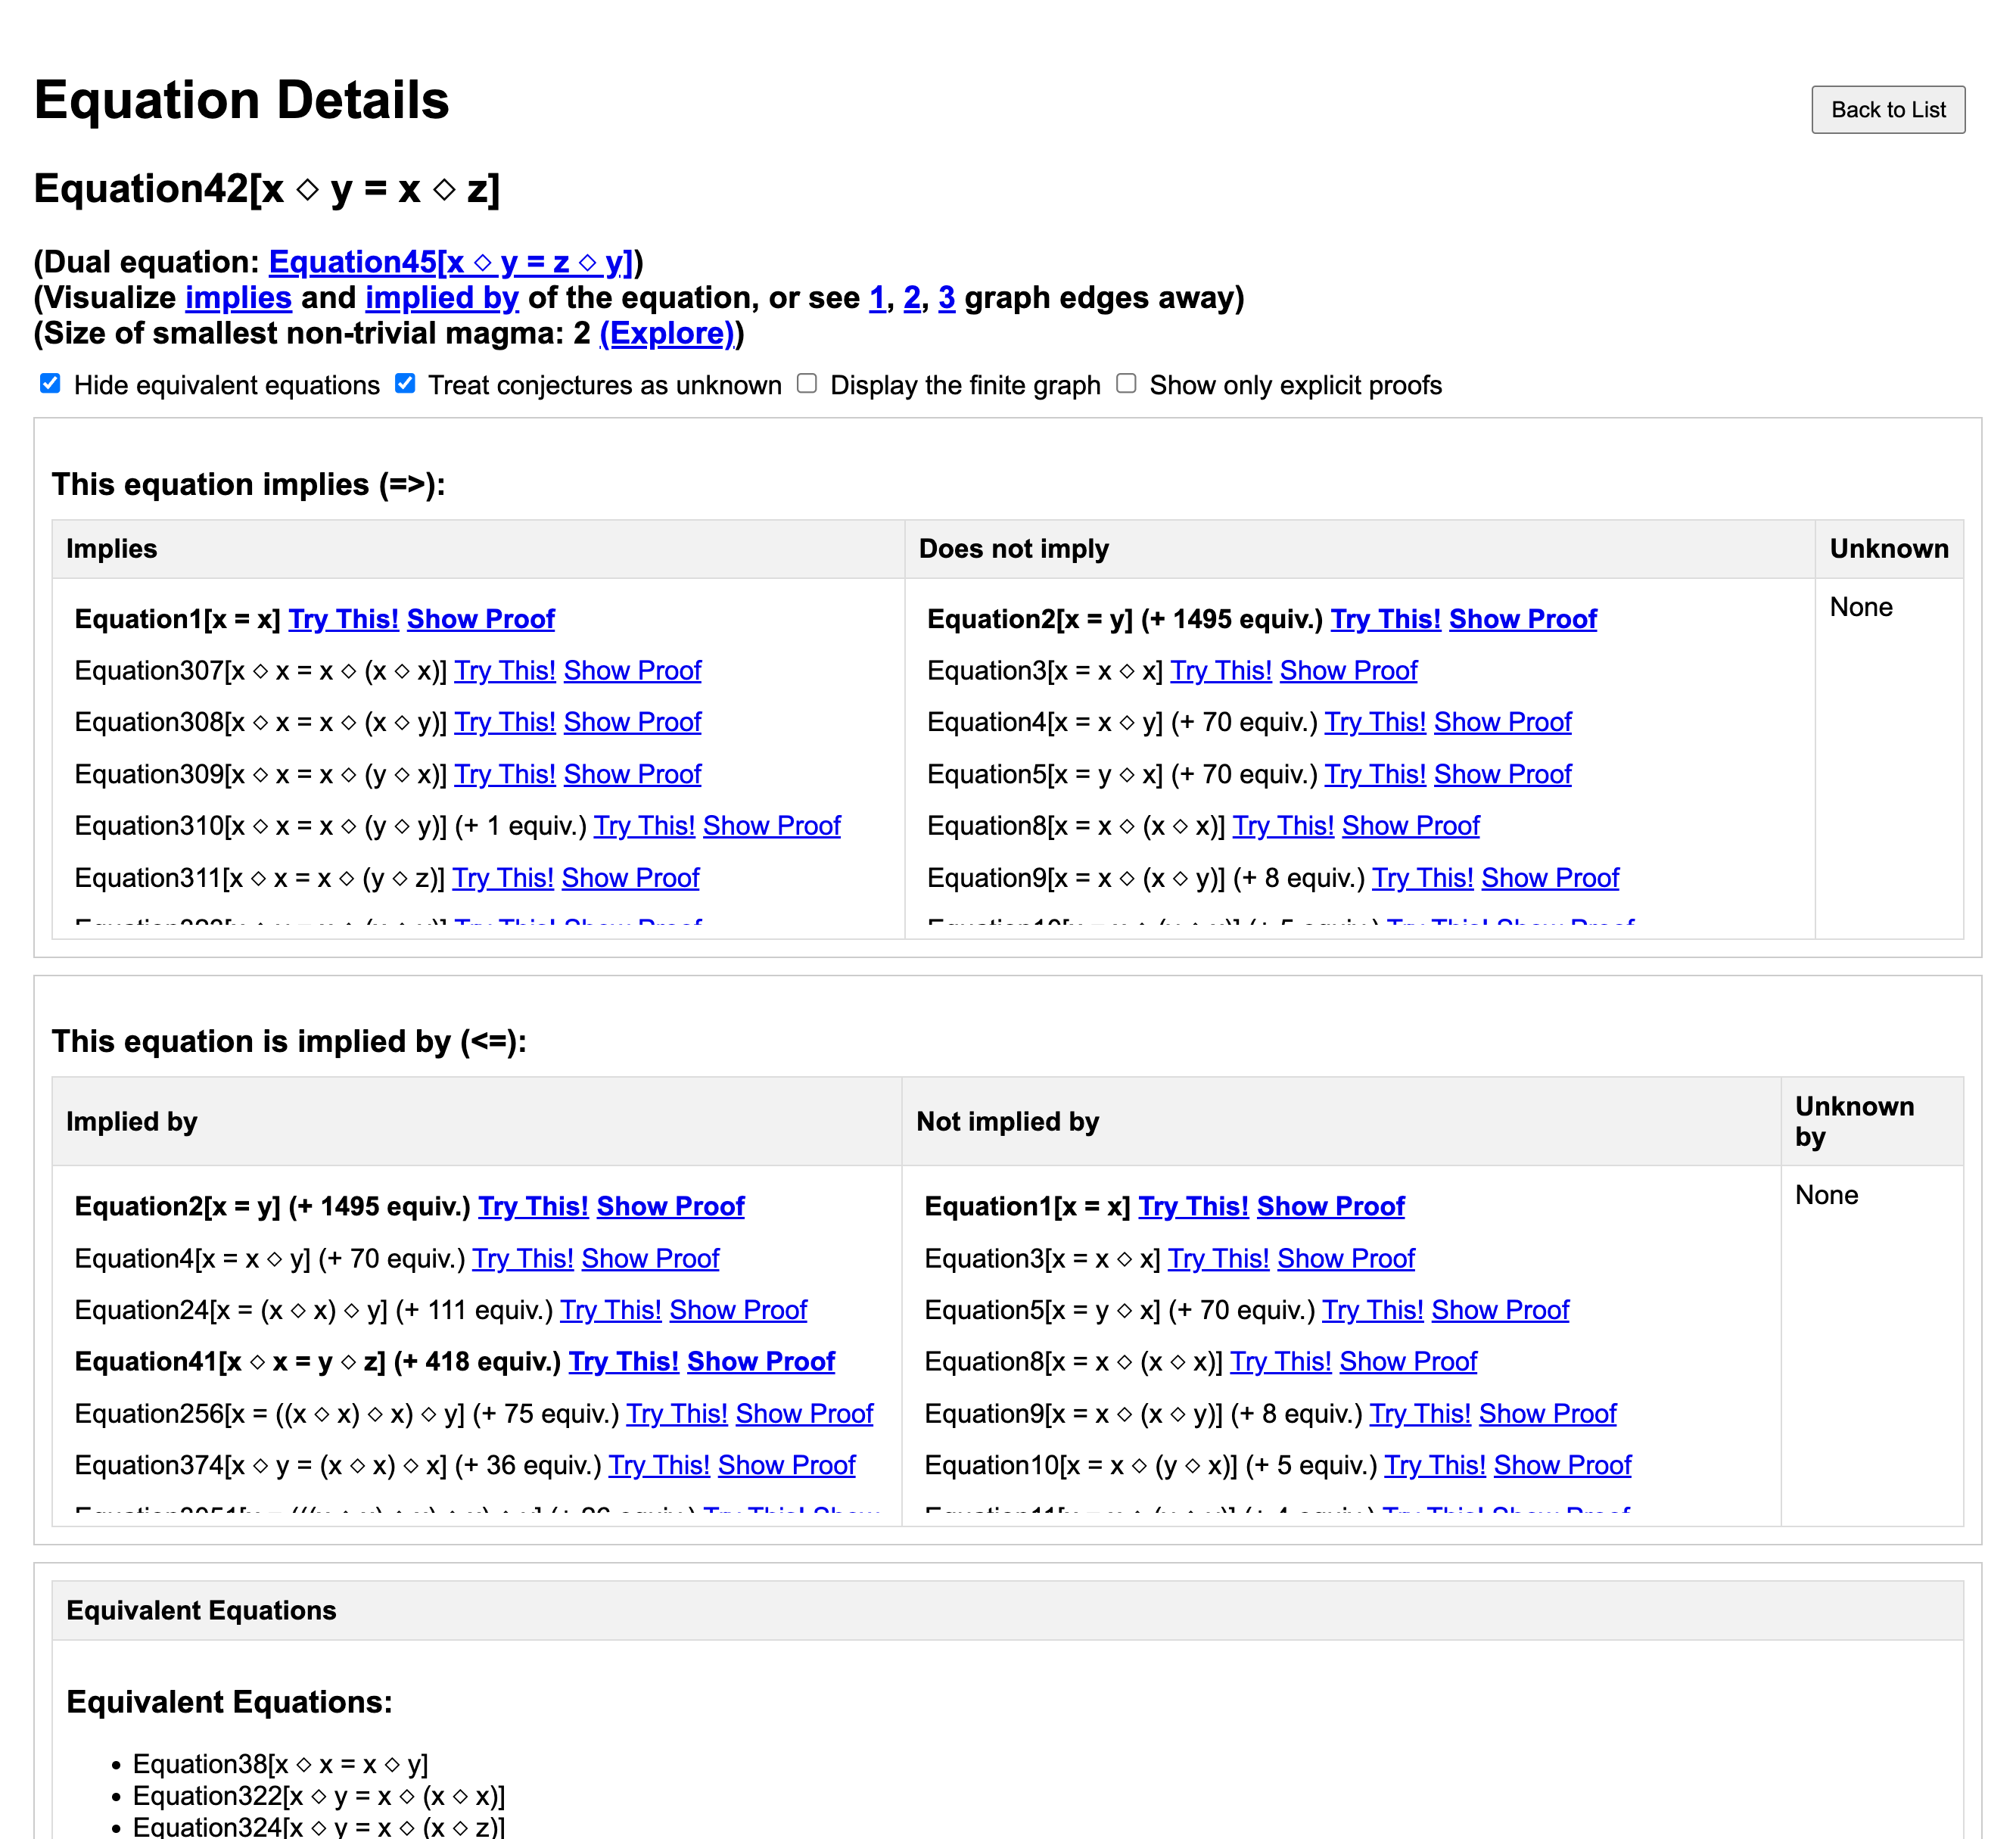
\includegraphics[width=0.85\textwidth]{GUI-equation-explorer.png}
  \caption{An example of the information displayed by the Equation Explorer for a specific equation.}
  \label{fig:screenshot-equation-explorer}
\end{figure}

The data for these tools is extracted directly from the Lean-formalized proofs in the project's GitHub repository, ensuring it always faithfully reflects the current state of progress. Additionally, the data is automatically updated with each code change using continuous integration (CI), eliminating the need for manual updates.

\section{Statistics and Experiments}

\note{TODO: Expand this sketch}

Data analysis of the implication graph

\begin{itemize}
    \item Mention the long chain 2 => 5 => 2499 => 2415 => 238 => 2716 => 28 => 2973 => 270 => 3 => 3715 => 375 => 359 => 4065 => 1 (discussed here).
\item What are the "most difficult" implications?
\item Is there a way to generate a standard test set of implication problems of various difficulty levels? Can one then use this to benchmark various automated and semi-automated methods? Challenge: how does one automatically assign a difficulty level to a given (anti-)implication?
\end{itemize}

See this for a preliminary data analysis of the impact of equation size and the number of variables.

Analyze the implication graph and discuss test sets of implication problems for benchmarking theorem provers. Challenge: How can one automatically assign a difficulty level to an implication?

\section{Data Management}

\note{TODO: expand this sketch}

Describe how data was handled during the project and how it will be managed going forward.


\section{Reflections}

\note{TODO: expand this sketch}

Testimonies from individual participants (but perhaps this is more suited for a retrospective paper). Utilize the thoughts and reflections thread.

Automation often overtook the rate of human progress, for instance in developing metatheorems. Does this create an opportunity cost? Raised as a possible discussion point here by Zoltan Kocsis.

\section{Conclusions and Future Directions}

This project successfully demonstrated that large-scale explorations of a space of mathematical statements---in this case, the implications or non-implications between selected equational laws---can be crowdsourced using modern collaboration platforms and proof assistants.  No single tool or method was able to study the entirety of this space, and many informal proofs generated contained non-trivial errors; but there were multiple techniques that could treat significant portions of the space, and through a collaborative effort combined with the proof validation provided by \emph{Lean}, one could synthesize these partial and fallible contributions into a complete and validated description of the entire implication graph.  While this particular graph was a comparatively simple structure to analyze, we believe that this paradigm could also serve as a model for future projects devoted to exploring more sophisticated large-scale mathematical structures.

Several factors appeared to be helpful in ensuring the success of the project, including the following:
\begin{itemize}
\item \textbf{A clearly stated primary goal, with an end condition and precise numerical metrics to measure partial completion.}  From the outset, there was a specific goal to attain, namely to completely determine and then formalize the implication graph on the original set of $4694$ laws.  Progress towards that goal could be measured by a number of metrics, such as the number of implications that were conjectured but unformalized, or not conjectured at all.   Such metrics allowed participants to see how partial contributions, such as formalizing a certain subset of implications, advanced the project directly towards its primary goal.  This is not to say that all activity was devoted solely towards this primary goal, but it did provide a coherent focus to help guide and motivate other secondary activities.
\item \textbf{A highly modular project}.  It was possible for any given coauthor to work on a small subset of implications and focus on a single proof technique, without needing to understand or rely upon other contributions to the project.  This allowed the work to be both parallelized and decentralized; many contributors launched their own investigations broadly within the framework of the project, without needing centralized approval or coordination.
\item \textbf{Low levels of required mathematical and formal prerequisites}.  The problems considered in the project did not require advanced mathematical knowledge (beyond a general familiarity with abstract algebra), nor a sophisticated understanding of formal proof assistants.  This permitted contributions from a broad spectrum of participants, including those without a graduate mathematical training, as well as mathematicians with no experience in proof formalization.  At a technical level, it also meant that formalization of proofs into \emph{Lean} could be done immediately once certain base definitions (such as \texttt{Magma}) were constructed.  This can be compared for instance with the recent formalization of the Polynomial Freiman--Ruzsa conjecture\footnote{\url{https://github.com/teorth/pfr}}, in which significant effort was expended in the first few days to settle on a suitable framework to formalize the mathematics of Shannon entropy.  While some more sophisticated formal structures (such as the syntactic description of laws as pairs of words in a \texttt{FreeMagma}) were later introduced in the project, it was relatively straightforward to refactor previously written code to be compatible with these structures as they were incorporated into the project.
\item \textbf{Variable levels of difficulty, and the amenability to partial progress.}  Traditional mathematics projects generally involve a small number of extremely hard problems, with incomplete progress on these problems being difficult to convert into clean partial results.  In contrast, the ETP studied a large number of problems with a very broad range of difficulty, so that even if a given proof strategy did not work for a given implication, it could be the case that there was some class of easier implications for which the strategy was successful.  This allowed for a means to validate such ideas, and allowed the project to build up a useful and diverse toolbox of proof techniques which became increasingly necessary to handle the final and most difficult implications in the project.  It also created a dynamic in which the project initially focused on easy techniques to resolve a significant fraction of the implications, gradually transitioning into more sophisticated methods that focused on a much smaller number of outstanding implications that had proven resistant (or even ``immune'') to all easier approaches.
\item \textbf{Centralized and standardized platforms for discussion, project management, and validation.}  While the project was decentralized at the level of the participant, there was a centralized location (a channel\footnote{\url{https://leanprover.zulipchat.com/\#narrow/channel/458659-Equational}} on the Lean Zulip) to discuss all aspects of the project, as well as a centralized repository\footnote{\url{https://github.com/teorth/equational_theories}} to track all contributions and outstanding issues, a centralized blueprint\footnote{\url{https://teorth.github.io/equational_theories/blueprint/}} to describe technical details of proofs to be formalized, and a single formal language (\emph{Lean}) to validate all contributions. A significant portion of the activity in the early stages of the project was devoted to setting out the standards and workflows for handling both the discussion and the contributions, in particular setting up a contributions page\footnote{\url{https://github.com/teorth/equational_theories/blob/main/CONTRIBUTING.md}} and adopting a code of conduct\footnote{\url{https://github.com/teorth/equational_theories/blob/main/CODE_OF_CONDUCT.md}}.  This gave some structure and predictability to what might otherwise be a chaotic effort.
\item \textbf{Development of custom visualization tools.}  As discussed in \Cref{sec:gui-sec}, several tools were developed (in part with AI assistance) to help visualize and navigate the implication graph while it was in a partial stage of development, allowing for participants to independently identify problems to work on, and to validate and use the contributions of other participants even before they were fully formalized.  For instance, a participant could propose a finite counterexample to an implication by posting a link to the magma in \emph{Finite Magma Explorer}, allowing for immediate validation of the counterexample, or use \emph{Equation Explorer} or \emph{Graphiti} to observe some interesting phenomenon in the implication graph that other participants could reproduce and study.
\item \textbf{Applicability of existing software tools.}  As described in \Cref{automated-sec}, many of the implications in the ETP were amenable to application of ``off-the-shelf'' automated theorem provers (ATPs); while some trial and error was needed to determine good choices of parameters, these tools could largely be applied directly to the project without extensive customization.  (However, the later transcription of ATP output into Lean was sometimes non-trivial.)
\item \textbf{Receptiveness to new techniques and tools.}  Crucially, the methods used to make progress on the project were not specified in advance, and contributions from participants with new ideas, techniques, or software tools that were not initially anticipated were welcomed.  For instance, the theory of canonizers (\Cref{canon-sec}) was not initially known to the first project participants, but was brought to the attention of the project by a later contributor.  Conversely, while there were hopes expressed early in the project that modern large language models (LLMs) could automatically generate many of the proofs required, it turned out in practice that other forms of automation, particularly ATPs, were significantly more effective at this task (at least if one restricted to publicly available LLMs), and the project largely moved away from the use of such LLMs (other than to help create the code for the visualization tools).
\end{itemize}

There are several mathematical and computational questions that could potentially be addressed in future work building upon the outcomes of ETP.  Here is a list of some possible such future directions.
\begin{enumerate}
  \item Does the law $\x \formaleq \y \op (\x \op ((\y \op \x) \op \y))$ \eqref{eq677} imply $\x \formaleq ((\x \op \x) \op \x) \op \x$ \eqref{eq255} for finite magmas? This is the last remaining implication (up to duality) for finite magmas to be resolved.  A number of partial results on this problem may be found at \url{https://teorth.github.io/equational_theories/blueprint/677-chapter.html}.
  \item Does the law $\x \formaleq \y \op (\y \op (\y \op (\x \op (\z \op \y))))$ \eqref{eq5093} have any infinite models? In \cite{Kisielewicz2} it was shown that it has no finite models, but the infinite model case was left as an open question.
  \item The ETP focused on determining relations $\E \models \E'$ between one law and another.  Could the same methods also systematically determine more complex logical relations, such as $\E_1 \wedge \E_2 \models \E_3$, for all laws $\E_1,\E_2,\E_3$ in a specified set?
  \item A key feature of finite magmas $\Magma$ is that they are surjunctive, in the sense that any definable map from $M$ to itself that is surjective, is also injective (or vice versa), where ``definable'' is with respect to the language of magmas.  Are there equational theories that admit surjunctive models, but yet do not have any finite models?
  \item Are there interesting examples of implications $\E_1 \models \E_2$ which are ``irreducible'' in the sense that there is no equational law $\E$ with $\E_1 \models \E \models \E_2$, other than those laws equivalent to either $\E_1$ or $\E_2$?
  \item How ``stable'' is a given law $\E$?  For instance, if a finite magma satisfies a law $\E$ some proportion $1-\eps$ of the time, with $\eps$ small, can the magma be perturbed into one that satisfies $\E$ exactly?  Related to this is the question of whether a law $\E$ is ``rigid'' or ``mutable'': is it possible to make a small number of modifications to a magma satisfying $\E$ in a way that still preserves $\E$?  Such properties helped suggest whether certain magma construction techniques, such as modifying a base magma, were likely to be successful.
\end{enumerate}

\subsection{Miscellaneous remarks}

It is possible that the timing in which certain proof methods were introduced into the project created some opportunity costs.  For instance, by deploying automated theorem provers at an early stage, we might have settled some implications that had more interesting human-readable proofs that we missed.  Similarly, we developed some sophisticated theory for the equation \eqref{eq854}, such as \Cref{unique-factorization}, that is now superseded by finite counterexamples; but had the finite counterexamples been discovered first, we would not have found the theoretical arguments.  It may be productive for future work to revisit some portions of the implication graph and locate alternate proofs and methods.


\section*{Acknowledgments}

We are grateful to the many additional participants to the Equational Theories Project for their
numerous comments and encouragement, with particular thanks to  Stanley Burris, Edward van de Meent and David Roberts.


\appendix

\section{Numbering system}\label{numbering-app}

In this section we record the numbering conventions we use for equational laws.

For this formal definition we use the natural numbers $0,1,2,\dots$ to represent and order indeterminate variables; however, in the main text, we use the symbols $\x,\y,\z,\w,\uu,\vv,\mathrm{r},\mathrm{s},\mathrm{t}$ instead (and do not consider any laws with more than eight variables).

To define the ordering we use on equational laws, we first consider the case where there is a single indeterminate $\ast$.
We place a well-ordering on words $w,w'$ with a single indeterminate $\ast$ by declaring $w > w'$ if one of the following holds:
\begin{itemize}
    \item $w$ has a larger order than $w'$.
    \item $w = w_1 \op w_2$ and $w' = w'_1 \op w'_2$ have the same order $n \geq 1$ with $w_1 > w'_1$.
    \item $w = w_1 \op w_2$ and $w' = w'_1 \op w'_2$ have the same order $n \geq 1$ with $w_1 = w'_1$ and $w_2 > w'_2$.
\end{itemize}
Thus, for instance
$$ \ast < \ast \op \ast < \ast \op (\ast \op \ast) < (\ast \op \ast) \op \ast.$$

We similarly place a well-ordering on equational laws $w_1 \formaleq w_2$ with a single indeterminate $\ast$ by declaring $w_1 \formaleq w_2 > w'_1 \formaleq w'_2$ if one of the following holds:
as follows:
\begin{itemize}
\item  $w_1 \formaleq w_2$ has a longer order than $w'_1 \formaleq w'_2$.
\item If $w_1 \formaleq w_2$ has the same order as $w'_1 \formaleq w'_2$, and $w_1 > w'_1$.
\item If $w_1 \formaleq w_2$ has the same order as $w'_1 \formaleq w'_2$, $w_1 = w'_1$, and $w_2 > w'_2$.
\end{itemize}
Thus for instance
$$ (\ast \op \ast \formaleq \ast \op (\ast \op \ast)) < (\ast \op \ast \formaleq (\ast \op \ast) \op \ast).$$

Finally for equational laws with alphabet $\x,\y,\z,\w,\uu,\vv,\mathrm{r},\mathrm{s},\mathrm{t}$, define the \emph{shape} of that law to be the law formed by replacing all indeterminates with $\ast$; for instance, the shape of \eqref{eq4512}, $\x \op (\y \op \z) = (\x \op \y) \op \z$, is $\ast \op (\ast \op \ast) \formaleq (\ast \op \ast) \op \ast$.  We then place a well-ordering $w_1 \formaleq w_2$ with indeterminates $\x,\y,\z,\w,\uu,\vv,\mathrm{r},\mathrm{s},\mathrm{t}$ by declaring $w_1 \formaleq w_2 > w'_1 \formaleq w'_2$ if one of the following holds:
\begin{itemize}
\item The shape of $w_1 \formaleq w_2$ is greater than the shape of $w'_1 \formaleq w'_2$.
\item $w_1 \formaleq w_2$ and $w'_1 \formaleq w'_2$ have the same shape, and the string of variables appearing in $w_1 \formaleq w_2$ is lower in the lexicographical ordering (using $\x < \y < \z < \w < \uu < \vv < \mathrm{r} < \mathrm{s} < \mathrm{t}$) than the corresponding string for $w'_1 \formaleq w'_2$.
\end{itemize}
Thus for instance any law of shape $\ast \op \ast \formaleq \ast \op (\ast \op \ast)$ is lower than any law of shape
$\ast \op \ast \formaleq (\ast \op \ast) \op \ast$.  Among the laws of shape $\ast \op \ast \formaleq \ast \op (\ast \op \ast)$, the lowest is $\x \op \x \formaleq \x \op (\x \op \x)$, which is less than (say) $\x \op \x \formaleq \y \op (\y \op \y)$, which is in turn less than $\x \op \y \formaleq \x \op (\x \op \x)$.

We say that two equational laws are \emph{definitionally equivalent}\footnote{This can be distinguished from the weaker notion of \emph{propositional equivalence} (mutual entailment) used in the rest of the paper.} if one can be obtained from another by some combination of relabeling the variables and applying the symmetric law $w_1 \formaleq w_2 \iff w_2 \formaleq w_1$.  For instance, $(0 \op 1) \op 2 \formaleq 1$ is definitionally equivalent to $0 \formaleq (1 \op 0) \op 2$.  We then replace every equational law with their minimal element in their definitional equivalence class, which can be viewed as the \emph{normal form} for that law; for instance, the normal form of $(0 \op 1) \op 2 \formaleq 1$ would be $0 \formaleq (1 \op 0) \op 2$.  Finally, we eliminate any law of the form $w \formaleq w$ other than $0 \formaleq 0$.  We then number the remaining equations $\Eq{1}, \Eq{2}, \dots$.  For instance, $\Eq{1}$ is the trivial law $0 \formaleq 0$, $\Eq{2}$ is the constant law $0 \formaleq 1$, $\Eq{3}$ is the idempotent law $0 \formaleq 0 \op 0$, and so forth.  Lists and code for generating these equations, or the equation number attached to a given equation, can be found in the ETP repository.

The number of equations in this list of order $n=0,1,2,\dots$ is given by
$$ 2, 5, 39, 364, 4284, 57882, 888365, \dots$$
(\url{https://oeis.org/A376640}).  The number can be computed to be
$$ C_{n+1} B_{n+2}/2$$
if $n$ is odd, $2$ if $n=0$, and
$$ (C_{n+1} B_{n+2}+ C_{n/2}(2D_{n+2}-B_{n+2}))/2 - C_{n/2} B_{n/2+1}$$
if $n > 2$ is even, where $C_n, B_n$ are the Catalan and Bell numbers, and $D_n$ is the number of partitions of $[n]$ up to reflection, which for $n=0,1,2,\dots$ is
$$ 1, 1, 2, 4, 11, 32, 117, \dots$$
(\url{https://oeis.org/A103293}).  A proof of this claim can be found in the ETP blueprint.  In particular, there are $4694$ equations of order at most $4$.

Below we record some specific equations appearing in this paper, using the alphabet $\x$, $\y$, $\z$, $\w$, $\uu$, $\vv$ in place of $0$, $1$, $2$, $3$, $4$, $5$, $\dots$ for readability.
\begingroup\allowdisplaybreaks
\begin{align}
    \x &\formaleq \x & \hbox{(Trivial law)} \label{eq1}\tag{E1} \\
    \x &\formaleq \y & \hbox{(Singleton law)} \label{eq2}\tag{E2} \\
    \x &\formaleq \x \op \x & \hbox{(Idempotent law)} \label{eq3}\tag{E3} \\
    \x &\formaleq \x \op \y & \hbox{(Left-absorptive law)} \label{eq4}\tag{E4} \\
    \x &\formaleq \y \op \x & \hbox{(Right-absorptive law)} \label{eq5}\tag{E5} \\
    \x &\formaleq \x \op (\y \op \x) \label{eq10}\tag{E10} \\
    \x &\formaleq \x \op (\y \op \y) & \hbox{(Right-unit squares law)} \label{eq11}\tag{E11} \\
    \x &\formaleq (\x \op \x) \op \x \label{eq23}\tag{E23} \\
    \x \op \x &\formaleq \y \op \y & \hbox{(Unipotence law)} \label{eq40}\tag{E40} \\
    \x \op \x &\formaleq \y \op \z & \hbox{(Constant law)} \label{eq41}\tag{E41} \\
    \x \op \y &\formaleq \y \op \x & \hbox{(Commutative law)} \label{eq43}\tag{E43} \\
    \x \op \y &\formaleq \z \op \w & \hbox{(Constant law)} \label{eq46}\tag{E46} \\
    \x &\formaleq \x \op (\x \op (\x \op \x)) \label{eq47}\tag{E47} \\
    \x &\formaleq \y \op (\y \op (\x \op \y))  \label{eq73}\tag{E73} \\
    \x &\formaleq (\x \op \x) \op (\x \op \x) \label{eq151}\tag{E151} \\
    \x &\formaleq (\y \op \x) \op (\x \op \z) & \hbox{(Central groupoid law)} \label{eq168}\tag{E168} \\
    \x &\formaleq (\x \op (\x \op \y)) \op \y \label{eq206}\tag{E206} \\
    \x &\formaleq ((\x \op \x) \op \x) \op \x \label{eq255}\tag{E255} \\
    \x \op \y &\formaleq \x \op (\y \op \z) & \hbox{(Right reduction law)} \label{eq327}\tag{E327} \\
    \x \op \y &\formaleq (\x \op \y) \op \y & \hbox{(Right idempotence law)} \label{eq378}\tag{E378} \\
    \x \op \y &\formaleq (\z \op \x) \op \y & \hbox{(Left reduction law)} \label{eq395}\tag{E395} \\
    \x &\formaleq \x \op (\x \op (\x \op (\y \op \x))) \label{eq413}\tag{E413} \\
    \x &\formaleq \y \op (\z \op (\x \op (\y \op \z))) & \hbox{(Tarski's axiom)} \label{eq543}\tag{E543} \\
    \x &\formaleq \y \op (\x \op ((\y \op \x) \op \y)) & \hbox{(Last open implication)} \label{eq677}\tag{E677} \\
    \x &\formaleq \x \op ((\x \op \x) \op (\x \op \x)) \label{eq817}\tag{E817} \\
    \x &\formaleq \x \op ((\y \op \z) \op (\x \op \z)) \label{eq854}\tag{E854}\\
    \x &\formaleq \x \op ((\y \op (\y \op \x)) \op \x) \label{eq1045}\tag{E1045} \\
    \x &\formaleq \x \op ((\y \op (\z \op \x)) \op \x) \label{eq1055}\tag{E1055} \\
    \x &\formaleq \y \op ((\y \op (\x \op \x)) \op \y) \label{eq1110}\tag{E1110} \\
    \x &\formaleq \y \op ((\y \op (\x \op \z)) \op \z) \label{eq1117}\tag{E1117} \\
    \x &\formaleq \y \op (((\x \op \y) \op \x) \op \y) \label{eq1286}\tag{E1286} \\
    \x &\formaleq (\y \op \x) \op (\x \op (\z \op \y)) & \hbox{(Weak central groupoids)}\label{eq1485}\tag{E1485} \\
    \x &\formaleq (\y \op \z) \op (\y \op (\x \op \z)) & \hbox{(Boolean groups)} \label{eq1571}\tag{E1571} \\
    \x &\formaleq (\x \op \x) \op ((\x \op \x) \op \x) \label{eq1629}\tag{E1629} \\
    \x &\formaleq (\x \op \y) \op ((\x \op \y) \op \y) \label{eq1648}\tag{E1648} \\
    \x &\formaleq (\x \op \y) \op ((\y \op \y) \op \z) \label{eq1659}\tag{E1659} \\
    \x &\formaleq (\y \op \x) \op ((\x \op \z) \op \z) & \hbox{(Equivalent to~\eqref{eq2})} \label{eq1689}\tag{E1689} \\
    \x &\formaleq (\y \op \y) \op ((\y \op \x) \op \y) \label{eq1729}\tag{E1729} \\
    \x &\formaleq (\y \op (\x \op (\y \op \x))) \op \y \label{eq2301}\tag{E2301} \\
        \x &\formaleq (\x \op ((\x \op \x) \op \x)) \op \x \label{eq2441}\tag{E2441} \\
        \x &\formaleq ((\y \op (\x \op \y)) \op \x) \op \y & \hbox{(Dual of \eqref{eq677})} \label{eq2910}\tag{E2910} \\
        \x \op \y &\formaleq \x \op (\y \op (\x \op \y)) \label{eq3316}\tag{E3316} \\
        \x \op \y &\formaleq (\x \op \z) \op (\y \op \z) \label{eq3737}\tag{E3737} \\
        \x \op \y &\formaleq (\x \op (\y \op \x)) \op \y \label{eq3925}\tag{E3925} \\
        \x \op (\y \op \x) &\formaleq \x \op (\y \op \z) \label{eq4315}\tag{E4315} \\
        \x \op (\x \op \x) &\formaleq (\x \op \x) \op \x & \hbox{(Cube-associativity law)} \label{eq4380}\tag{E4380} \\
        \x \op (\y \op \y) &\formaleq (\y \op \y) \op \x & \hbox{(Central squares law)} \label{eq4482}\tag{E4482} \\
        \x \op (\y \op \z) &\formaleq (\x \op \y) \op \z & \hbox{(Associative law)} \label{eq4512}\tag{E4512} \\
        \x \op (\y \op \z) &\formaleq (\y \op \z) \op \x & \hbox{(Central products law)} \label{eq4531}\tag{E4531} \\
        \x &\formaleq \y \op (\y \op (\y \op (\x \op (\z \op \y)))) \label{eq5093}\tag{E5093} \\
        \x &\formaleq \y \op (\z \op ((\y \op \x) \op (\z \op (\y \op \z)))) & \hbox{(Eisenstein modules)} \label{eq85914} \tag{E85914} \\
        \x &\formaleq \y \op (\z \op ((\y \op \z) \op (\w \op (\x \op \w)))) & \hbox{(Gaussian modules)} \label{eq86082} \tag{E86082} \\
        \x &\formaleq (\y \op ((\x \op \y) \op \y)) \op (\x \op (\z \op \y)) & \hbox{(Sheffer stroke)} \label{eq345169}\tag{E345169}
\end{align}
We also list some order-$8$ characterizations of group division relevant for \Cref{higman-neumann}.
\begin{align}
        \x &\formaleq \y \op ((((\x \op \x) \op \x) \op \z) \op (((\x \op \x) \op \y) \op \z)) & \hbox{(McCune law)} \label{eq42302852}\tag{E42302852} \\
        \x &\formaleq \y \op ((((\x \op \x) \op \x) \op \z) \op (((\y \op \y) \op \y) \op \z)) & \label{eq42302946}\tag{E42302946} \\
        \x &\formaleq \y \op ((((\y \op \y) \op \x) \op \z) \op (((\y \op \y) \op \y) \op \z)) & \hbox{(Higman--Neumann law)} \label{eq42323216}\tag{E42323216} \\
        \x &\formaleq (\y \op \y) \op (\y \op ((\x \op \z) \op (((\x \op \x) \op \y) \op \z))) & \hbox{(in finite magmas)} \label{eq67953597}\tag{E67953597} \\
        \x &\formaleq ((\y \op \y) \op \y) \op ((((\x \op \x) \op \x) \op \z) \op (\y \op \z)) & \label{eq89176740}\tag{E89176740} \\
        \x &\formaleq ((\y \op \y) \op ((\x \op \z) \op \x)) \op ((\z \op \w) \op (\x \op \w)) & \label{eq102744082}\tag{E102744082} \\
        \x &\formaleq ((\y \op \y) \op (\y \op (\x \op (((\y \op \y) \op \y) \op \z)))) \op \z & \hbox{(McCune law)} \label{eq147976245}\tag{E147976245}
\end{align}
\endgroup

% \section{Proofs of Theoretical Results}

\note{Provide the interesting proofs mentioned in the results section, while routine proofs can refer to the blueprint or Lean.}

\section{Author contributions}

In a \href{https://github.com/teorth/equational_theories/blob/main/paper/contributions.md}{companion document} to this paper, the contributions of each author of this paper to the ETP are described, following the standard CRediT categories\footnote{\url{https://credit.niso.org/}}.  Below are the affiliations and grant acknowledgments of individual participants.


\begin{itemize}
    \item Matthew Bolan: University of Toronto, matthew.bolan@mail.utoronto.ca
    \item Joachim Breitner: Lean FRO, mail@joachim-breitner.de, ORCID 0000-0003-3753-6821
    \item Jose Brox: IMUVA-Mathematics Research Institute, Universidad de Valladolid, josebrox@uva.es. Supported by a postdoctoral fellowship “Convocatoria 2021” funded by Universidad de Valladolid, and partially supported by grant PID2022-137283NB-C22 funded by MCIN/AEI/10.13039/501100011033 and ERDF “A way of making Europe”
    \item Mario Carneiro: Chalmers University of Technology \& Gothenburg University, Sweden, marioc@chalmers.se
    \item Martin Dvorak: Institute of Science and Technology Austria, martin.dvorak@matfyz.cz
    \item Andr\'es Goens: TU Darmstadt, andres.goens@tu-darmstadt.de
    \item Aaron Hill: Unaffiliated, aa1ronham@gmail.com
    \item Harald Husum: harald.husum@gmail.com
    \item Hern\'an Ibarra Mejia: hernan@ibarramejia.com
    \item Zoltan A. Kocsis: University of New South Wales, z.kocsis@unsw.edu.au
    \item Bruno Le Floch: CNRS and Laboratoire de Physique Th\'eorique et Hautes \'Energies, Sorbonne Universit\'e, blefloch@lpthe.jussieu.fr
    \item Lorenzo Luccioli: University of Bologna, lorenzo.luccioli2@unibo.it
    \item Douglas McNeil: dsm054@gmail.com
    \item Alex Meiburg: Perimeter Institute for Theoretical Physics / University of Waterloo Institute for Quantum Computing, teqtp@ohaithe.re
    \item Pietro Monticone: University of Trento, pietro.monticone@studenti.unitn.it
    \item Pace P. Nielsen: Department of Mathematics, Brigham Young University, pace@math.byu.edu
    \item Giovanni Paolini: University of Bologna, g.paolini@unibo.it
    \item Marco Petracci: University of Bologna, marco.petracci@studio.unibo.it
    \item Bernhard Reinke: Aix-Marseille Université, bernhard.reinke@univ-amu.fr
    \item David Renshaw: Institute for Computer-Aided Reasoning in Mathematics, renshaw@icarm.io
    \item Marcus Rossel: Barkhausen Institut, marcus.rossel@barkhauseninstitut.org
    \item Cody Roux: Amazon Web Services, cody.roux@gmail.com
    \item J\'er\'emy Scanvic, Laboratoire de Physique, École Normale Supérieure de Lyon, jeremy.scanvic@ens-lyon.fr
    \item Shreyas Srinivas: CISPA Helmholtz Center for Information Security, Saarbr\"{u}cken, Germany. shreyas.srinivas@cispa.de.
    \item Anand Rao Tadipatri: University of Cambridge, art71@cam.ac.uk
    \item Terence Tao: Department of Mathematics, UCLA, tao@math.ucla.edu. Supported by the James and Carol Collins Chair, the Mathematical Analysis \& Application Research Fund, and by NSF grants DMS-2347850, and is particularly grateful to recent donors to the Research Fund, ORCID 0000-0002-0140-7641.
    \item Vlad Tsyrklevich: vlad@tsyrklevi.ch
    \item Fernando Vaquerizo-Villar: Biomedical Engineering Group, University of Valladolid, and CIBER de Bioingeniería, Biomateriales y Nanomedicina, Instituto de Salud Carlos III, fernando.vaquerizo@uva.es
    \item Daniel Weber: Ben-Gurion University of the Negev, weberdan@post.bgu.ac.il
    \item Fan Zheng: ...

\end{itemize}


\bibliographystyle{plain}
\bibliography{references}

\end{document}
